\documentclass[11pt, letterpaper]{book}%tipo

\usepackage{template}
\usepackage{lipsum}

\usepackage{
  amsmath, amsthm, 
  amssymb,amsfonts,
  cancel,
  stmaryrd,esint, 
  xfrac, upgreek, 
  braket, slashed
}

%==========Comandos Personales y macros===========
\usepackage{cancel}
\def\RR{\mathbb{R}}
\def\NN{\mathbb{N}}
\def\ZZ{\mathbb{Z}}
\def\II{\mathbb{I}}
\def\QQ{\mathbb{Q}}
\def\CC{\mathbb{C}}
\DeclareSymbolFont{matha}{OML}{txmi}{m}{it}% txfonts
\DeclareMathSymbol{\varv}{\mathord}{matha}{118}%var v
\DeclareMathSymbol{\varl}{\mathord}{matha}{108}%var l
\def\lag{\mathcal{L}}
\def\Dcov{\mathcal{D}}
%-----Derivadas-------
\def\dy{\,\,d\!y\,}
\def\dx{\,\,d\!x\,}
\def\dz{\,\,d\!z\,}
\def\dv{\,\,d\!\varv\,}
\def\dt{\,\,d\!t\,}
\def\ask{\overset{?}=}
\renewcommand{\check}{
  \overset{
    \checkmark\!\!\!\!\!\!\!\checkmark}{\!\!\!=}
}
\usepackage{rotating}
\newcommand{\der}[3] [2]{\frac{d\! #2}{d\! #3}}
\newcommand{\ders}[3] [2]{\frac{d^2\! #2}{d\! #3^2}}
\newcommand{\dert}[3] [2]{\frac{d^3\! #2}{d\! #3^3}}
\newcommand{\derf}[3] [2]{\frac{d^4\! #2}{d\! #3^4}}
\newcommand{\dern}[3] [2]{\frac{d^n\! #2}{d\! #3^n}}
\newcommand{\dpr}[3] [2]{\frac{\partial\!\, #2}{\partial\!\, #3}}
\newcommand{\dprs}[3] [2]{\frac{\partial^2\! #2}{\partial\! #3^2}}
\newcommand{\dprt}[3] [2]{\frac{\partial^3\! #2}{\partial\! #3^3}}
\newcommand{\dprf}[3] [2]{\frac{\partial^4\! #2}{\partial\! #3^4}}
\newcommand{\dprn}[3] [2]{\frac{\partial^n\! #2}{\partial\! #3^n}}
\newcommand{\dfr}[3] [2]{\frac{\delta\! #2}{\delta\! #3}}
\newcommand{\dfrs}[3] [2]{\frac{\delta^2\! #2}{\delta\! #3^2}}
\newcommand{\dfrt}[3] [2]{\frac{\delta^3\! #2}{\delta\! #3^3}}
\newcommand{\dfrf}[3] [2]{\frac{\delta^4\! #2}{\delta\! #3^4}}
\newcommand{\dfrn}[3] [2]{\frac{\delta^n\! #2}{\delta\! #3^n}}
%----otros comandos
\def\Max{\text{Max}}
\def\diag{\text{diag}}
\def\sign{\text{sign}}
\def\entonces{\;\;\;\,\Longrightarrow\;\;\;\,}
% \newcommand{\Abs}[1]{\left\vert#1\vphantom{y}\right\vert}%
% \newcommand{\abs}[1]{\left\vert#1\vphantom{y}\right\vert}%
\newcommand{\Eva}[1]{\left.#1\vphantom{\frac yy}\right\vert}%
\newcommand{\cor}[1]{\left[ #1\vphantom{y}\right]}
\newcommand{\Fac}[1]{\left( #1\vphantom{y}\right)}
\newcommand{\fac}[1]{\left( #1\vphantom{y}\right)}
\def\mode{\displaystyle}
\newcommand{\vph}{\mode\vphantom{\dfrac{y^y}{y^y}}}
\newcommand{\cint}{\displaystyle C\kern-1em\int}
\usepackage{multicol}
\usepackage{multirow}
\usepackage{bigstrut}
\usepackage{graphicx}
\usepackage{epstopdf}
\usepackage{subcaption}
\usepackage[detect-all]{siunitx}
\usepackage[%
	backend=bibtex8,
	style=numeric-comp,
	sorting=none,
	autocite=inline
	]{biblatex}
\addbibresource{references.bib}

\usepackage{etex, tikz, tikz-3dplot, xcolor}
\usetikzlibrary{
  decorations.pathreplacing,
  decorations.pathmorphing,
  decorations.markings,
  arrows, fadings,
  positioning,
  shapes, shadows,
  shapes.geometric,
  calc
}
\usepackage{pgfplots}
\pgfplotsset{compat=1.18}
\usepackage{feynmp-auto}
\usepackage{tcolorbox}
\tcbset{colback=black!5!white, colframe=black!75!black, fonttitle=\bfseries}
\definecolor{Black}{rgb}{0.0, 0.0, 0.0}
\usepackage{pdfpages}
\usepackage{tocbibind}
\usepackage{listings}

\title{Machine Learning-enhanced feasibility studies on the production of new particles with preferential couplings to third generation fermions at the LHC}
\author{Cristian Fernando Rodríguez Cruz}
% Default values
\university{Universidad de los Andes}
\faculty{Faculty of Sciences}
\department{Department of Physics}
\researchgroup{Uniandes - High Energy Physics Research Group}
\lineofinvestigation{Phenomenology of Particle Physics}
\advisor{Prof. Andrés Florez}
\advisoraffiliation{Universidad de los Andes}
\coadvisor{Prof. Joel Jones-Perez}
\coadvisoraffiliation{Pontificia Universidad Católica del Perú}
\degree{Doctor in Sciences - Physics}
\citycountry{Bogotá D.C., Colombia}
\thesistype{Thesis}
\date{\today. Pre-alpha version}
\def\tev{\, {\rm TeV}}
\def\gev{\, {\rm GeV}}
\def\fb{\, {\rm fb}}
\def\lq{{\rm LQ}}
\def\bq{{\rm b}}
\def\tq{{\rm t}}
\def\wb{{\rm W}}
\def\zb{{\rm Z}}
\def\pt{p_{\rm{T}}}
\def\el{{\rm e}}
\def\Bm{{\rm B}}
\begin{document}
\frontmatter

\maketitle

\begin{abstract}
The Standard Model (SM) of particle physics is the most successful framework for describing the subatomic world. It is continuously tested in experiments worldwide, with the Large Hadron Collider (LHC) being the flagship project in this endeavor. One of the primary goals of the LHC is to precisely measure SM parameters and search for deviations that could signal new physics.  

In recent years, reported anomalies, such as those in $B$-meson decays from LHCb, BaBar, and Belle experiments, along with the potential discrepancy in the muon's magnetic moment ($g-2$) from Fermilab, suggest a violation of lepton flavor universality (LFU). These observations provide a compelling window into physics beyond the SM. Among the proposed SM extensions to explain LFU violation, many introduce new particles with preferential couplings to third and second-generation fermions. Popular candidates include heavy states such as $Z'$ bosons, $\phi'$ scalars, and leptoquarks (LQs), among others.

This work presents two phenomenological studies proposing different strategies to probe new models, such as the $4321$ \cite{Florez2023}, $U(1)_{T^3_R}$ \cite{Qureshi:2024naw}, that extend the SM particle content to explain clues on LFU violation. The studies use benchmark scenarios in which the structure of the model and the couplings of the new particle fields determine preferential interactions with second- and third-generation SM fermions. The hypothetical signal and background samples are generated using Monte Carlo simulations, emulating the current running conditions of the LHC and the performance of the CMS detector. The expected sensitivity for the different signal models under study is obtained by performing a detailed analysis of the available (non-excluded) experimental phase-space, boosted by  machine learning (ML) techniques to optimize the discovery potential for these exotic states.
\end{abstract}

% \begin{dedication}
% to be added
% \end{dedication}

% \begin{acknowledgements}
% to be added
% \end{acknowledgements}



\tableofcontents

\mainmatter
\chapter*{Introduction}\addcontentsline{toc}{chapter}{\numberline{}\spacedlowsmallcaps{Introduction}}
%\lipsum
$ $ 

The pursuit of a fundamental description of nature's building blocks and their interactions is a central endeavor of modern physics. This quest has led to the development of the Standard Model (SM) of particle physics, a quantum field theory that encapsulates our current understanding of the subatomic world. With breathtaking precision, the SM describes the electromagnetic, weak, and strong nuclear forces and classifies all known elementary particles. Its triumphs are undeniable, crowned by the landmark discovery of the Higgs boson at the Large Hadron Collider (LHC) in 2012, which confirmed the mechanism for generating mass and represented the final piece of the SM puzzle.

Yet, for all its success, the Standard Model is universally acknowledged to be an incomplete theory. It offers no candidate for dark matter, cannot account for the asymmetry between matter and antimatter in the universe, does not incorporate gravity, and leaves the mass of the Higgs boson itself unnaturally unstable under quantum corrections—a problem known as the hierarchy problem. These profound theoretical shortcomings provide a clear motivation for physics beyond the Standard Model (BSM). However, the most compelling guide for this search has always come from experimental data itself.

The primary mission of the LHC is not only to consolidate the SM but to probe its boundaries and discover new physics. While no direct evidence of new particles has been found so far, a series of subtle but persistent discrepancies—termed ``anomalies''—have emerged from experiments worldwide, suggesting a potential crack in the SM's foundation.

A particularly intriguing set of these anomalies points towards a violation of Lepton Flavor Universality (LFU). The SM predicts that the electroweak force couples with identical strength to the three charged leptons (electrons, muons, and taus), a fundamental principle known as LFU. The most significant and long-standing hints of LFU violation come from measurements of semileptonic $B$-meson decays. The ratios $R(D^{(*)}) = \mathcal{B}(B \to D^{(*)} \tau \nu_\tau) / \mathcal{B}(B \to D^{(*)} \ell \nu_\ell)$, where $\ell$ is a muon or electron, have been measured by the BaBar, Belle, and LHCb collaborations to consistently exceed the SM predictions by a combined significance of approximately $3\sigma$-$4\sigma$. This deviation suggests that $B$ mesons are more likely to decay to a final state containing a tau lepton than the SM allows, providing a compelling hint of new physics that couples preferentially to the third generation. Furthermore, the longstanding discrepancy in the muon's anomalous magnetic moment ($g-2$), recently confirmed with increased precision by the Fermilab experiment, adds another layer of intrigue, as it also hints at new physics potentially coupled preferentially to the second generation.

While each anomaly individually requires careful scrutiny, their collective persistence has generated significant excitement, as they seem to point towards new physics that breaks lepton flavor universality, potentially involving enhanced couplings to heavier fermions.


The pattern of these LFU-violating anomalies has inspired a vast landscape of theoretical models extending the SM. A common thread among the most promising explanations is the introduction of new heavy particles that mediate interactions with non-universal couplings to the different generations of fermions. This generational hierarchy is crucial to evade tight constraints from precision measurements on electrons (first generation) while affecting processes involving muons and taus.

Prominent candidates for such new states include:
\begin{itemize}
    \item \textbf{Leptoquarks (LQs):} Bosons that can decay to both a quark and a lepton, offering a natural tree-level explanation for the $B$-decay anomalies, particularly for $R(D^{(*)})$.
    \item \textbf{$Z'$ Bosons:} New neutral vector bosons that could mediate flavor-changing neutral currents.
    \item \textbf{New Scalars:} Beyond the Higgs, such as the $\phi'$ scalar.
\end{itemize}

In this thesis, we contextualize and present two of our phenomenological studies that propose different strategies to probe new physics models, such as the $4321$~\cite{Florez2023} and $U(1)_{T^3_R}$~\cite{Qureshi:2024naw} models, which extend the SM particle content to explain the observed LFU violation. These models introduce new particles with preferential couplings to second and third-generation fermions, making them prime candidates for explaining the experimental anomalies.

The experimental challenge lies in probing these models at the LHC. The proposed new particles are often heavy, leading to low production rates, and their decay signatures are complex and overwhelmed by enormous Standard Model backgrounds. Discovering them requires not just more data but innovative analysis strategies that can maximize the sensitivity to these exotic and rare processes.

This thesis presents two dedicated phenomenological studies that propose and develop novel strategies to probe the $4321$ and $U(1)_{T^3_R}$ models at the LHC. The work is situated at the intersection of theoretical model-building and experimental high-energy physics.

The core methodology of this research involves:
\begin{enumerate}
    \item Defining \textbf{benchmark scenarios} within each model, selecting specific mass points and coupling structures that explain the LFU anomalies while remaining experimentally viable.
    \item Using \textbf{Monte Carlo simulation} to accurately generate the hypothetical signal processes alongside the dominant SM background processes, emulating the run conditions of the LHC and the performance of the CMS detector.
    \item Performing a detailed analysis of the available experimental phase-space, employing advanced \textbf{Machine Learning (ML) techniques} to construct discriminators that optimally separate the rare signal events from the background.
    \item Deriving the \textbf{expected sensitivity} for each model, establishing the exclusion limits or discovery potential that the LHC experiments could achieve with the current dataset.
\end{enumerate}

The structure of this thesis is as follows. We begin by establishing the theoretical foundation with a review of the Standard Model in Chapter 2. Chapter 3 then details the experimental context, describing the LHC and the CMS detector, and introduces the general analysis techniques employed. The original phenomenological work of this thesis is presented in the subsequent chapters: Chapter 4 details a search for new physics in the process $pp \to t\bar{t}\mu^+\mu^-$, while Chapter 5 presents a search for vector leptoquarks in the process $pp \to \tau^+\tau^- + b\text{-jets}$. Finally, Chapter 6 concludes by summarizing our findings and discussing their implications for the field, along with an outlook on future prospects.
\chapter{Standard Model of Particle Physics}\label{ch:sm}

The Standard Model (SM) of particle physics is a quantum field theory (QFT) that describes matter as fermionic particles and their fundamental interactions. The forces are incorporated through the gauge principle, where force-carrying particles---vector bosons with spin one, arising from the adjoint representation of symmetry groups (\textit{gauge groups})---mediate the interactions between matter particles~\parencite{greiner2000relativistic,pokorski2000gauge}. However, this elegant formulation is not sufficient to account for particle masses. These are generated through Yukawa interactions, which are scalar-fermion couplings between the Higgs field and the fermion fields. While the Yukawa interactions themselves are not gauge interactions, their allowed structure---specifically, which fermions they can couple and their transformation properties---is strictly dictated by the gauge symmetry of the theory. This combined framework of gauge and Yukawa sectors successfully describes three of the four fundamental forces in nature.

In this chapter, we contextualize the SM by introducing the basic concepts of quantum field theory, including the notion of fields and symmetries. We then present the particle content of the SM, its gauge group, and the Lagrangian density that describes its dynamics. The Higgs mechanism and its role in providing mass to the weak gauge bosons and fermions are also discussed. Finally, we address the main deficiencies of the SM and review the experimental evidence that motivates the search for physics beyond the SM.

\section{Fields}
Relativistic quantum fields are degrees of freedom in QFT. Formally, they are \textit{operator-valued functions on spacetime that transform under a representation of the Lorentz group on an invariant subspace}~\parencite{Tong1995}. The different representations of the Lorentz group are mainly characterized by their spin, and their fields obey a different equation of motion (see table~\ref{tab-repLorentz2}). 

In classical field theory, a variational principle is established which generates the equations that govern the dynamics of the different fields in a theory, \textit{the equations of motion}. Hamilton's principle, or principle of minimal action, indicates that all possible physical configurations for a set of fields $\varphi^I$, with $I=1,2,3,\cdots,n$, are those for which the action $S$ is  minimal~\parencite{Goldstein,jose1998classical}:
\begin{equation}\label{eq-action}
	S=\int \mathcal{L}(\varphi^I,\partial_\mu\varphi^I) d^4x.
\end{equation}
Here, $d^4x=dx^0dx^1 dx^2dx^3$ and $x\equiv(ct,x^1,x^2,x^3)\equiv(x^0,x^1,x^2,x^3)\in\mathcal{M}^4$, are the space-time coordinates in the Minkowskian spacetime ($\mathcal M^4$), and the function $\lag(\varphi^I,\partial_\mu\varphi^I)$ is called \textit{the Lagrangian density} of a theory~\parencite{greiner2000relativistic,Goldstein}. The problem in classical field dynamics is to find the functions $\varphi^I(x)$ in a space-time $\mathcal{M}^4$, fixing their boundary conditions. The solution to this classical problem is given by the Euler-Lagrange equations:
\begin{equation}\label{eq_EulerLag}
	\dpr{\mathcal{L}}{\varphi^I}-\dpr{}{x^\mu}\dpr{\lag}{\fac{\partial_\mu \varphi^I}}=0,
\end{equation}
and they are used to obtain the equations of motion of the set of fields $\varphi^I$~\parencite{jose1998classical}. 

While in classical field theory the Euler–Lagrange equations directly determines the dynamics of the system, in QFT the approach changes: if we adopt the path-integral formulation~\parencite{martinez2002,Weinberg}, the idea of an equation of motion vanishes and we move on to searching for correlations between free particle states. However, the notion of action remains the cornerstone in the description of these observables.

Explicitly, the correlation functions are calculated through the Lehmann-Symanzik-Zimmermann (LSZ) reduction formula, which connects these correlators with physical scattering amplitudes. These are computed from the path integral~\parencite{greiner1996qft,peskin}:
\begin{equation}
	\begin{aligned}
		Z[J]&=\braket{\text { out, } 0| 0, \text { in }}
		\\&=\mathcal{N}\int \mathcal{D}(\varphi, \bar{\varphi})  e^{i S[\varphi]} e^{i \int J_I\varphi^I  d^{4} x}
		\\&=\mathcal{N}\int \mathcal{D}(\varphi, \bar{\varphi})  e^{i \int d^{4} x \mathcal{L}} e^{i \int J_I\varphi^I  d^{4} x},
	\end{aligned}
\end{equation}
taken over the space of fields $\varphi$ with an appropriate measure $\mathcal{D}(\varphi, \bar{\varphi})$ and normalized by $\mathcal{N}$. The quantity $Z$ is known as the partition function of the theory and gives the transition amplitude from the initial vacuum $\ket{0,\text{ in}}$ to the final vacuum $\ket{0,\text{ out}}$ in the presence of a source $J(x)$ producing particles~\parencite{birrell75900}.


\begin{center}
    \begin{tabular}{|l|c|c|l|}\hline\bigstrut
        Name							& Field				& Spin & Free-Lagrangian	\\\hline\hline\bigstrut
        Klein-Gordon				&	$\phi$					& $0$			&	$\lag=\frac{1}{2}\fac{\partial^\mu \phi\partial_\mu \phi-m^2 \phi\phi}$						\\\hline\bigstrut
        Dirac								& $\chi$			& $1/2$	&$\lag=\bar\chi\fac{i\pmb\gamma^\mu \partial_\mu -m\pmb 1}\chi$\\\hline\bigstrut
        Proca (Massive Vector)	        & $A^\mu$ 		& $1$		&$\lag=-\frac{1}{4} F^{\mu\nu} F_{\mu\nu} + \frac{1}{2}m^2 A^\mu A_\mu $\\\hline
    \end{tabular}
	\captionof{table}{Some relevant representations of the Lorentz group in  $4$-dimensional space-time. In this notation $\eta_{\mu\nu}=\diag(1,-1,-1,-1)$, $\pmb \gamma^\mu$ are the Dirac matrices, $F_{\mu \nu}=\partial_{\mu} A_{\nu}-\partial_{\nu} A_{\mu}$ is the abelian field strength tensor. All equations are written in natural units with $c=\hbar=1$. Fields are shown in their standard representations.}\label{tab-repLorentz2}
\end{center}

Therefore, the dynamics, at both the classical and quantum levels, are entirely determined by the Lagrangian density. For free fields (i.e., non-interacting), the Lagrangian is quadratic in the fields and the path integral can be evaluated exactly. Tab.~\ref{tab-repLorentz2} records the Lagrangian density for these free fields. However, to describe physics, we must include interactions, which render the path integral impossible to compute exactly.

The framework of \textit{perturbation theory} addresses this by expanding the interaction part of the Lagrangian as a power series. This expansion is organized using \textit{Feynman diagrams}, which provides a pictorial representation of each term, and a set of \textit{Feynman rules}, which provides a precise dictionary to translate these diagrams into mathematical expressions for scattering amplitudes~\parencite{peskin,Weinberg}. The importance of these rules cannot be overstated, as they are the practical computational tools of perturbative QFT.


In this paradigm, our task is to propose a Lagrangian density for a set of fields that correctly models the propagation and interactions of fundamental particles. The free part defines the particle content and propagators, while the interaction part defines the vertices and possible scattering processes.

\subsection{Interactions and Symmetries} 

The structure of the Lagrangian density in a quantum field theory is not arbitrary; it is constrained by fundamental principles that ensure the theory is physically consistent and mathematically well-defined. These principles act as ``rules'' that guide the construction of viable theories. In what follows, we systematically develop these constraints, starting from the practical requirements of perturbation theory and building up to the fundamental symmetry principles.

To perform calculations, we typically split the Lagrangian into a free part, which describes non-interacting fields, and an interaction part:
\begin{equation}
    \mathcal{L} = \mathcal{L}_0 + \mathcal{L}_{\text{int}}.
\end{equation}
This splitting is the starting point for perturbation theory. In the path integral formulation, the generating functional $Z[J]$ can then be expressed as an operator acting on the free functional $Z_0[J]$:
\begin{equation}
    Z[J] = \mathcal{N} \exp\left[i \int d^4x\, \mathcal{L}_{\text{int}}\left(-i \frac{\delta}{\delta J(x)}\right)\right] Z_0[J].
\end{equation}
The exponential operator generates an infinite series known as the perturbation series. The $n$-point correlation function is found by taking functional derivatives of $Z[J]$ with respect to the sources $J(x_i)$ and setting $J=0$. Each term in this series is represented by a \textbf{Feynman diagram}, whose components are:

\begin{itemize}
    \item \textbf{External Lines:} Represent incoming and outgoing physical particles.
    \item \textbf{Internal Lines:} Represent virtual particles propagating between interactions, corresponding to the free-field propagators derived from $\mathcal{L}_0$.
    \item \textbf{Vertices:} Represent interactions, derived from the terms in $\mathcal{L}_{\text{int}}$. Each vertex has an associated coupling constant and enforces momentum conservation.
\end{itemize}

\begin{figure}[h!]
    \centering
    \begin{fmffile}{feyngraphs/feyngraph0}
        \vspace{0.5cm}
        \begin{fmfgraph*}(120,80)
            \fmfleft{i1,i2}
            \fmfright{o1,o2}
            
            % External incoming lines
            \fmf{fermion}{i1,v1}
            \fmf{fermion}{i2,v2}
            
            % Internal propagator
            \fmf{photon,label=$\gamma$,label.side=left}{v1,v2}
            
            % External outgoing lines
            \fmf{fermion}{v1,o1}
            \fmf{fermion}{v2,o2}
            
            % Labels for external particles
            \fmflabel{$e^-$}{i1}
            \fmflabel{$e^+$}{i2}
            \fmflabel{$e^-$}{o1}
            \fmflabel{$e^+$}{o2}
            
            % Vertex labels
            \fmfv{label=$v_1$,label.angle=180,label.dist=0.3cm}{v1}
            \fmfv{label=$v_2$,label.angle=0,label.dist=0.3cm}{v2}
        \end{fmfgraph*}
        \vspace{0.5cm}
    \end{fmffile}
    \caption{Example of a Feynman diagram for $e^+e^- \to e^+e^-$ scattering. \textbf{External lines} (solid arrows at the edges) represent the incoming and outgoing electrons and positrons. The \textbf{internal line} (wavy line) represents the virtual photon propagator. The \textbf{vertices} ($v_1$ and $v_2$) represent the electromagnetic interaction points where the coupling constant $e$ (electric charge) enters and momentum is conserved.}
    \label{fig:feynman-components}
\end{figure}

For this perturbation series to be a predictive computational tool, it must yield finite physical results. However, individual terms in the series (i.e., individual Feynman diagrams) often lead to divergent integrals when loop corrections are included. The key is that in a \textit{renormalizable} theory, these divergences from all diagrams can be systematically absorbed into a finite number of parameters (like masses and coupling constants) through a redefinition procedure known as renormalization. It is important to note that while individual Feynman diagrams may diverge, the requirement is that the combination of all contributions at a given order yields finite, physically meaningful results after renormalization.

This requirement of renormalizability imposes a powerful constraint on the form of $\mathcal{L}_{\text{int}}$. Through power-counting arguments, one finds that only operators of mass dimension $\leq 4$ lead to renormalizable interactions. In natural units, where $\mathcal{L}$ has dimension $[\text{mass}]^4$, this means that $\mathcal{L}_{\text{int}}$ can be expressed as a truncated polynomial containing only terms up to dimension 4. Specifically, this allows Yukawa couplings (dim 4), quartic scalar interactions (dim 4), and gauge interactions (dim 4), while forbidding non-renormalizable operators like $\phi^6$ (dim 6). Higher-dimensional operators are still allowed in effective field theories, but they correspond to interactions that are suppressed at low energies and signal the presence of new physics at higher scales~\parencite{peskin,Weinberg}.

This is why we express $\mathcal{L}_{\text{int}}$ as a truncated polynomial: renormalizability demands that we include only a finite set of operators with dimension $\leq 4$, ensuring that the theory remains predictive at all accessible energy scales.

An additional crucial requirement is the \textit{stability of the vacuum}. For a theory to be physically meaningful, it must possess a stable ground state. This is ensured by demanding that the scalar potential, which governs the self-interactions of scalar fields, is bounded from below. If the potential were unbounded, the system could lower its energy indefinitely by evolving toward field configurations of ever-greater magnitude, meaning no stable vacuum would exist.

For a renormalizable theory, the scalar potential can contain at most quartic terms. A general scalar potential for a set of scalar fields $\{\phi_i\}$ takes the form:
\begin{equation}
    V(\phi_i) = \sum_i \mu_i^2 |\phi_i|^2 + \sum_{i,j} \lambda_{ij} |\phi_i|^2 |\phi_j|^2 + \cdots
\end{equation}
where the ellipsis denotes possible cubic and mixed quartic terms allowed by the symmetries of the theory. The stability condition requires that the quartic couplings $\lambda_{ij}$ satisfy certain positivity constraints to ensure that $V \to +\infty$ as $|\phi_i| \to \infty$ in any direction in field space. This is why the scalar potential is a polynomial of at most order four: renormalizability forbids higher-order terms, and stability demands that the quartic terms dominate at large field values with the correct sign.

It is important to note that this condition must hold not just at tree-level but also at the quantum level, as running couplings can change sign at different energy scales, potentially leading to metastability or instability of the vacuum.

A fundamental requirement from quantum mechanics is \textit{Hermiticity}: the Lagrangian density must be Hermitian to ensure that observables are real and the time evolution of the theory is unitary~\parencite{pall,peskin}. This is the most basic constraint that quantum theory imposes on the Lagrangian. Without Hermiticity, the theory would predict complex-valued probabilities and violate the fundamental probabilistic interpretation of quantum mechanics.

Beyond the quantum mechanical requirement of Hermiticity, special relativity imposes a fundamental constraint: \textit{Poincaré invariance}. This symmetry demands that the equations of motion remain the same in all inertial frames. Mathematically, this is implemented by requiring the action to be globally invariant under Poincaré transformations~\parencite{pall}. Equivalently, the Lagrangian density must transform as a Lorentz scalar and may change under translations at most by a total derivative~\parencite{jose1998classical}.\marginpar{\footnotesize In QFT, Poincaré invariance is assumed to be global. Promoting it to a local symmetry leads to gravity, with spin-2 fields (the graviton) as mediators. Perturbatively, such a theory is not renormalizable, so it lacks predictivity at high energies, although it can still be understood as an effective field theory.}

This constraint is extremely powerful: it eliminates all possible interaction terms that would depend on the choice of reference frame. For instance, terms that explicitly depend on spacetime coordinates or preferred directions are forbidden. Furthermore, \textit{dimensional analysis} places additional restrictions. In natural units, $\mathcal{L}$ carries dimensions of mass to the fourth power ($[\mathcal{L}] = [\text{mass}]^4$), which corresponds with an energy density. Combined with Lorentz invariance, this means that the interaction terms must be constructed from Lorentz-covariant combinations of fields and their derivatives, with the correct overall mass dimension.

The symmetries discussed so far—Poincaré invariance, Hermiticity, and dimensional analysis—are universal requirements that any relativistic quantum field theory must satisfy. However, they still leave a vast array of possible interaction terms. To further constrain the Lagrangian and to describe the fundamental forces of nature, we must consider \textit{internal symmetries}: transformations that act on the fields' internal degrees of freedom rather than on spacetime coordinates.

Internal symmetries can be either \textit{global} (where the transformation parameters are constant throughout spacetime) or \textit{local} (gauge symmetries, where the parameters can vary from point to point). The procedure for constructing gauge theories—where global symmetries are ``promoted'' to local ones by introducing gauge fields—is systematic and will be described in detail below. This gauge principle has proven to be the most powerful organizing principle in particle physics, determining not only which interactions are realized in nature but also their precise mathematical structure.

A classical symmetry of the Lagrangian may not always survive the process of quantization. If it fails to do so, it is said to be anomalous. \textit{Chiral anomalies}, specifically, arise from the regularization of fermion loops in triangle diagrams and can break gauge symmetries at the quantum level. Since gauge symmetry is the very principle that dictates the form of interactions and removes unphysical states, its violation would destroy the renormalizability and unitarity of the theory. Therefore, the particle content must be carefully chosen so that these potential anomalies cancel among fermions, a non-trivial condition famously satisfied by the quarks and leptons of the Standard Model~\parencite{peskin,Weinberg,bertlmann1996anomalies}.

In summary, the construction of a consistent relativistic quantum field theory proceeds through a hierarchy of constraints:
\begin{enumerate}
	\item \textbf{Perturbative renormalizability:} power-counting arguments restrict operators to mass dimension $\leq 4$, ensuring $\mathcal{L}_{\text{int}}$ is a truncated polynomial.
	\item \textbf{Vacuum stability:} the scalar potential must be bounded from below, requiring appropriate positivity conditions on quartic couplings.
	\item \textbf{Hermiticity:} quantum mechanics demands $\mathcal{L}$ be Hermitian for real observables and unitary evolution.
	\item \textbf{Poincaré invariance:} special relativity requires the action to be invariant under Lorentz transformations and translations, eliminating frame-dependent terms.
	\item \textbf{Internal symmetries:} global and gauge symmetries further constrain the form of interactions and determine the structure of fundamental forces.
	\item \textbf{Anomaly cancellation:} the particle content must be chosen such that chiral anomalies cancel, preserving gauge symmetry at the quantum level.
\end{enumerate}

These constraints drastically reduce the number of possible terms in the Lagrangian. The renormalizable interaction structures that survive are limited to: Yukawa couplings between fermions and scalars, quartic scalar self-interactions, and gauge interactions between matter fields and vector bosons. The precise form of these interactions is then determined by the internal (gauge) symmetries of the theory, which we now describe in detail.

The procedure is systematic: first, the spin$-0$ and spin$-1/2$ fields are organized into representations of a unitary (gauge) group $G$, such that the Lagrangian density is globally invariant under $G$. This global symmetry is then ``promoted'' to a \textit{local symmetry} (where the group parameters can vary in spacetime) by replacing the ordinary derivatives $\partial_\mu$ with \textit{covariant derivatives} $\Dcov_\mu$ that incorporate new \textit{gauge fields} $B_\mu^A$~\parencite{pokorski2000gauge,freedman2012supergravity, Gallego2016,VanProeyen1999,Martin2012}.
This ``promotion'' is described in more detail below.

Given a Lagrangian density $\lag(\varphi^I, \partial_\mu \varphi^I)$, where $I$ is an index enumerating the different fields $\varphi^{I}$ in the model, it is said to be \textit{globally symmetric} under unitary transformations if the action remains invariant under field variations. At infinitesimal level, these variations are given by:
\begin{equation}
	\delta_G \varphi^I = i\theta^A (T_A)^I_J \varphi^J,
\end{equation}
where $\theta^{A}$ are constant parameters of the transformation and the $T_{A}$ are the generators of the group $G$ in the appropriate representation. The corresponding finite unitary transformation is
\begin{equation}
	\mathcal{U}_G \equiv U(\theta)=\exp(i\theta^A T_A).
\end{equation}
Note that the $T_A$  generators  satisfy the same Lie algebra of the group $G$:
\begin{equation}
	[T_A, T_B] = i f_{AB}^{\;\;C}T_C,
\end{equation}
where $f_{AB}^{\;\;C}$ are the structure constants of $G$.

To promote the global symmetry to a local one ($\theta^A \to \theta^A(x)$), the ordinary derivative $\partial_\mu$ is replaced by a \textit{covariant derivative} $\Dcov_\mu$. This new derivative is designed to transform covariantly under the gauge group, meaning $\Dcov_\mu \varphi \to U(x) (\Dcov_\mu \varphi)$, so that the kinetic terms $\lag_{\text{kin}} \sim (\Dcov_\mu \varphi)^\dagger (\Dcov^\mu \varphi)$ remain invariant. This is achieved by introducing a gauge field $B_\mu^A$ for each generator $T_A$ and defining:
\begin{equation}
	\Dcov_\mu = \partial_\mu - i g B_\mu^A T_A,
\end{equation}
where $g$ is the gauge coupling constant. The transformation law for the gauge fields that ensures the covariant transformation of $\Dcov_\mu$ is:
\begin{equation}
	\delta B_\mu^A = \partial_\mu \theta^A + g f_{BC}{}^A \theta^B B_\mu^C.\label{eq:gauge-transformation}
\end{equation}

The introduction of the gauge fields $B_\mu^A$ requires the addition of a kinetic term for them to the Lagrangian. This is constructed from the \textit{field strength tensor} $F_{\mu\nu}^A$, defined as the curvature of the covariant derivative:
\begin{equation}
	F_{\mu\nu}^A T_A = -\frac{i}{g} [\Dcov_\mu, \Dcov_\nu] = \partial_\mu B^A_\nu - \partial_\nu B^A_\mu + g f_{BC}{}^A B^B_\mu B^C_\nu.
\end{equation}
The gauge-invariant kinetic Lagrangian is then:
\begin{equation}
	\lag_{\text{gauge}} = -\frac{1}{4} \delta_{AB} F^A_{\mu\nu} F^{\mu\nu B}.
\end{equation}
Often, the rescaling $B_\mu^A \to g B_\mu^A$ is performed, which moves the coupling constant $g$ from the kinetic term to the covariant derivative, resulting in the more conventional form $\Dcov_\mu = \partial_\mu - i g B_\mu^A T_A$ and $\lag_{\text{gauge}} = -\frac{1}{4g^2} \delta_{AB} F^A_{\mu\nu} F^{\mu\nu B}$.


A general, archetypal Lagrangian, embodying these structures, can be written as:
\begin{equation}\label{eq:generic-renorm-lag}
	\mathcal{L} = -\frac{1}{4} F_{\mu \nu}^A F^{A \mu \nu} + i \bar{\psi}^i \gamma^\mu \mathcal{D}_\mu \psi^i + \left(\bar{\psi}_L^j \, \Gamma^j_k \, \Phi \, \psi_R^k + \text{h.c.}\right) + |\mathcal{D}_\mu \Phi|^2 - V(\Phi)
\end{equation}
The terms correspond to: the kinetic term for gauge fields ($F_{\mu \nu}^A$), the kinetic term for fermions $\psi^i$, the Yukawa interactions between left- and right-handed fermions and scalars ($\Gamma^j_k$ is a Yukawa coupling matrix and $\Phi$ is a scalar field), the kinetic term for scalars, and the scalar potential $V(\Phi)$. For a renormalizable and  stable theory $V(\Phi) = \mu^2 |\Phi|^2 + \lambda |\Phi|^4$ with $\lambda > 0$.

Note the absence of explicit mass terms for the gauge fields ($\sim M^2 B_\mu B^\mu$) and fermions ($\sim m \bar{\psi}\psi$). These are forbidden by gauge invariance and for chiral fermions. Mass terms can be generated via spontaneous symmetry breaking, as discussed below.

It is important to emphasize that while the Yukawa interactions $\bar{\psi}_L^j \, \Gamma^j_k \, \Phi \, \psi_R^k$ do not involve gauge bosons directly, their structure is nonetheless \textit{completely determined by the gauge symmetry}. Specifically, gauge invariance dictates which fermion fields can couple to which scalar fields, and constrains the form of the coupling matrix $\Gamma^j_k$. For a Yukawa term to be gauge-invariant, the product $\bar{\psi}_L^j \, \Phi \, \psi_R^k$ must be a singlet under the gauge group. This requirement arises because the left-handed and right-handed fermions typically transform in different representations of the gauge group, and the scalar field $\Phi$ must carry the appropriate quantum numbers to make the overall combination invariant. In the Standard Model, for instance, the left-handed fermions are $SU(2)_L$ doublets while the right-handed fermions are singlets, and the Higgs doublet provides the necessary quantum numbers to form gauge-invariant Yukawa couplings. Thus, even though Yukawa interactions are scalar-mediated rather than gauge-mediated, the gauge principle is the fundamental organizing principle that determines their allowed structure.

\subsubsection{Example}
To illustrate these concepts, let us consider a renormalizable theory with a real scalar $\phi$ and a Dirac spinor $\psi$, and suppose that this theory is globally invariant under $U(1)$ phase transformations, i.e. the fields $\varphi\in\{\phi,\psi\}$ transform as $\varphi\mapsto e^{i\theta \hat Q}\varphi $ such that $\hat Q \psi = q \psi$ and $\hat Q \phi=0$. The free Lagrangian density is
\begin{equation}
	\mathcal L_{\text{free}}=\frac{1}{2} \partial^{\mu} \phi \partial_{\mu} \phi-\frac{1}{2}\mu^2\phi^2+\bar{\psi}(i \gamma_\mu  \partial^\mu-m) \psi.
\end{equation}
\marginpar{\footnotesize Note that for this vector-like $U(1)$ theory, the explicit fermion mass term $m\bar{\psi}\psi$ is gauge-invariant. This will not be the case for chiral gauge theories like the Standard Model.}

To add globally symmetric interaction terms, we must consider operators of mass dimension $\leq 4$. The most general renormalizable Lagrangian, invariant under the global $U(1)$ symmetry, is
\begin{equation}
	\begin{aligned}
		\mathcal L_{\text{global}}&=\frac{1}{2} \partial^{\mu} \phi \partial_{\mu} \phi-V(\phi)+\bar{\psi}(i \gamma_\mu  \partial^\mu-m) \psi + k_1 \phi\bar\psi\psi,
		\\
		V(\phi)&=\frac{1}{2}\mu^2\phi^2 +\frac{\alpha}{3!}\phi^3+\frac{\lambda}{4!}\phi^4.
	\end{aligned}
\end{equation}
The cubic and quartic terms in $V(\phi)$ are allowed as $\phi$ is neutral. The Yukawa coupling $k_1 \phi\bar\psi\psi$ is also gauge-invariant since the charges of $\bar\psi$, $\phi$, and $\psi$ sum to zero ($-q + 0 + q = 0$).

Promoting the global symmetry to a local one ($\theta \to \theta(x)$) requires introducing a gauge field $A_\mu$ and replacing ordinary derivatives with covariant derivatives:
\begin{equation}
	\mathcal D_\mu\varphi=(\partial_{\mu}-i g A_\mu\hat Q )\varphi
	\quad\Longrightarrow\quad
	\begin{cases}
		\mathcal D_\mu\phi=\partial_\mu \phi, & (\text{since } \hat Q\phi=0)\\
		\mathcal D_\mu\psi=(\partial_\mu - i g q A_\mu) \psi.
	\end{cases}
\end{equation}
The field strength tensor for the abelian $U(1)$ field is defined as $F_{\mu\nu} = \partial_\mu A_\nu - \partial_\nu A_\mu$. The locally invariant Lagrangian is then:
\begin{multline}
	\mathcal L_{\text{local}}=\frac{1}{2} \mathcal D^{\mu} \phi \mathcal D_{\mu} \phi-V(\phi)
	+\bar{\psi}i \gamma_\mu  \mathcal D^{\mu} \psi - m \bar{\psi}\psi
	+ k_1 \phi\bar\psi\psi-\frac{1}{4} F_{\mu\nu}F^{\mu\nu}.
\end{multline}


With these ingredients and principles, we are now equipped to understand the structure of the SM Lagrangian, which will be discussed in the next section.

\begin{figure}[h!]
    \centering
    \begin{subfigure}[b]{0.48\textwidth}
        \centering
        \begin{fmffile}{feyngraphs/feyngraph1} 
			\vspace{0.5cm}
            \begin{fmfgraph*}(80,60)
                \fmfleft{i1}
                \fmfright{o1,o2}
                
                \fmf{dashes,tension=2.0}{i1,v1}
                \fmf{fermion}{o1,v1}
                \fmf{fermion}{v1,o2}

                \fmflabel{$\phi$}{i1}
                \fmflabel{$\bar\psi$}{o1}
                \fmflabel{$\psi$}{o2}
            \end{fmfgraph*}
			\vspace{0.5cm}
        \end{fmffile}
        \caption{Yukawa coupling with a scalar $\phi$.}
        \label{fig-yukawa-scalar}
    \end{subfigure}
    \hfill
    \begin{subfigure}[b]{0.48\textwidth}
        \centering
        \begin{fmffile}{feyngraphs/feyngraph2}
			\vspace{0.5cm}
            \begin{fmfgraph*}(80,60)
                \fmfleft{i1}
                \fmfright{o1,o2}
                
                \fmf{photon,tension=2.0}{i1,v1}
                \fmf{fermion}{o1,v1}
                \fmf{fermion}{v1,o2}

                \fmflabel{$\gamma$}{i1}
                \fmflabel{$\bar\psi$}{o1}
                \fmflabel{$\psi$}{o2}
            \end{fmfgraph*}
			\vspace{0.5cm}
        \end{fmffile}
        \caption{Interaction with a photon $\gamma$.}
        \label{fig-qed-photon}
    \end{subfigure}
	\begin{subfigure}[b]{0.48\textwidth}
        \centering
		\begin{fmffile}{feyngraphs/feyngraph3}
			\vspace{1.0cm}
			\begin{fmfgraph*}(80,60)
				\fmfleft{i1}
				\fmfright{o1,o2}

				\fmf{dashes}{i1,v1}
				\fmf{dashes}{v1,o1}
				\fmf{dashes}{v1,o2}

				\fmflabel{$\phi$}{i1}
				\fmflabel{$\phi$}{o1}
				\fmflabel{$\phi$}{o2}
			\end{fmfgraph*}
			\vspace{0.5cm}
		\end{fmffile}
		\caption{Triple scalar coupling.}
		\label{fig-triple-scalar}
	\end{subfigure}
	\begin{subfigure}[b]{0.48\textwidth}
        \centering
		\begin{fmffile}{feyngraphs/feyngraph4}
			\vspace{1.0cm}
			\begin{fmfgraph*}(80,60)
				\fmfleft{i1,i2}
				\fmfright{o1,o2}

				\fmf{dashes}{i1,v1}
				\fmf{dashes}{i2,v1}
				\fmf{dashes}{v1,o1}
				\fmf{dashes}{v1,o2}

				\fmflabel{$\phi$}{i1}
				\fmflabel{$\phi$}{i2}
				\fmflabel{$\phi$}{o1}
				\fmflabel{$\phi$}{o2}
			\end{fmfgraph*}
			\vspace{0.5cm}
		\end{fmffile}
		\caption{Quartic scalar coupling.}
		\label{fig-quartic-scalar}
	\end{subfigure}
    \caption{Feynman diagrams for Yukawa coupling, gauge boson coupling and quartic scalar coupling.}
\end{figure}
 % Fields
\section{Standard Model}

{$ $ \scriptsize \hfill Fragment extracted and adapted from~\parencite{robinson2011symmetry}}

In 1965, Tomonaga, Feynman, and Schwinger were awarded the Nobel Prize for their independent formulation of Quantum Electrodynamics (QED)~\parencite{1972physics}. Their work established renormalization as a consistent method to separate infinities from finite, physically meaningful results in quantum field theory. QED provided predictions, such as the anomalous magnetic moment of the electron, that later experiments confirmed with remarkable precision~\parencite{1674-1137-40-10-100001, PhysRev.75.486}. It became the prototypical example of a successful quantum field theory.

This success, however, did not extend to other fundamental interactions. The weak interaction was described by the chiral $V-A$ model, in which processes like beta decay were represented by four-fermion contact terms. This framework was not renormalizable: divergences could not be absorbed into a finite set of parameters, restricting its validity to low energies. A fundamental description within the quantum field theory framework was still missing.

The issue was linked to the short-range character of the weak and strong forces. In quantum field theory, the range of an interaction depends on the mass of its mediating boson. A massless boson, such as the photon, generates a long-range force with an inverse-square dependence. A massive boson, in contrast, produces a Yukawa potential of the form $\exp(-mr)/r$, which falls off rapidly with distance. A consistent theory of the weak interaction therefore required massive gauge bosons.

Here lay the apparent obstacle. A mass term for a gauge boson, such as $m_{A}^{2} A_{\mu} A^{\mu}$ in the Lagrangian, explicitly breaks gauge invariance, since it is not preserved under the transformation $A_{\mu} \mapsto A_{\mu} + \partial_{\mu}\epsilon$. This seemed to rule out gauge theories as candidates for describing short-range forces. The problem was recognized early on. For instance, in a 1954 seminar where Chen Ning Yang introduced non-Abelian gauge theories, Wolfgang Pauli objected that assigning masses to the gauge bosons would violate gauge invariance, and without such masses the theory could not describe nuclear forces. This skepticism reflected a widely shared view: gauge symmetry appeared incompatible with short-range interactions.

The resolution of this problem came from two developments that allowed gauge bosons to behave as if they had mass, without explicitly breaking gauge symmetry:
\begin{enumerate}
    \item \label{list:sol_mass_1} The Higgs mechanism. In this framework, a scalar field permeates the vacuum. While the underlying Lagrangian remains gauge invariant, the vacuum state does not respect this symmetry. Gauge bosons interacting with this vacuum acquire mass in a renormalizable way. This mechanism explains the masses of the $W$ and $Z$ bosons.
    \item \label{list:sol_mass_2} Dynamical mass generation in non-Abelian gauge theories. In Quantum Chromodynamics (QCD), gluons and nearly massless quarks are confined into hadrons with substantial masses. The appearance of a mass gap is a nonperturbative consequence of confinement. Understanding this mechanism in a rigorous way is at the core of the Yang–Mills existence and mass gap Millennium Prize problem.
\end{enumerate}

The Standard Model (SM) incorporates both solutions. Electroweak theory relies on the Higgs mechanism (\ref{list:sol_mass_1}), which provides a renormalizable description of the weak interaction. For the strong interaction, QCD employs dynamical mass generation (\ref{list:sol_mass_2}), where most of the mass of hadrons arises from confinement rather than from the small quark masses introduced by the Higgs field.

\subsection{Particle Content and Gauge Group}

First, let us talk about the chiral nature of particles: Massive half-spin particles are described at the fundamental level by a Dirac spinorial field, see table \ref{tab-repLorentz2}. However, Dirac spinors do not transform under an irreducible representation of the Lorentz group. Spinors can be decomposed into two components that do transform under irreducible representations of the Lorentz group: two \textit{Weyl spinors}. The left and right chiral projectors, $P_L$ and $P_R$, take a Dirac spinor and project it onto each of these invariant subspaces. For a massless Dirac spinor, the left and right components are dynamically decoupled, \textit{i.e.} which are independent fields obeying independent Lagrangian densities; for example, the left component of a massless spinor has the Lagrangian $\lag=-i\bar\psi\slashed{\partial}P_L\psi$ (For more details see Appendix A at~\parencite{CRodriguezUPTC}). 

The discovery of parity asymmetry in radioactive decays~\parencite{PhysRev.105.1413} indicates that the chiral description of weak interactions couples differently to the left and right chiral components of half-spin particles. Indeed, the chirality of the fermionic spectrum is possibly one of the deepest properties of the Standard Model. Describing particles in terms of Dirac spinors, it means that left- and right-chirality components actually have different EW quantum numbers. This is compatible with a gauge symmetry only if half-spin particles are considered to be massless, at least without a Dirac mass $m \overline{f_{R}} f_{L}+\text { h.c.}$ Nevertheless, half-integer spin fundamental particles, such as the electron, have a well-measured mass. Therefore, the reconciliation of chiral asymmetry and mass lies in the Higgs mechanism, where the masses of the particles result from an effective Yukawa coupling with a scalar, the Higgs boson.

With this in mind, the SM has a content of matter fields from three generations (or families) of quarks $q$ and leptons $\ell$, described as Weyl 2-component spinors, with the structure
\begin{equation}
	q_{L}=\left(
		\begin{array}{c}
			u_{L}^{i} \\
			d_{L}^{i}
		\end{array}
	\right), 
	u_{R}^{i}, d_{R}^{i}, 
	\quad \ell_L=\left(
		\begin{array}{c}
			\nu_{L}^{i} \\
			e_{L}^{i}
		\end{array}
	\right), e_{R}^{i} ; \quad i=1,2,3 .
\end{equation}
All these particles transform under a group $U$(1) with different associated (hyper)charges.
The doublets formed by the left components of the fields transform under the representation of two components of a $SU$(2) group. The right components do not transform under SU(2), therefore they are singlets.
In addition, each quark in $q_{L}$ transforms as color triplets under $SU$(3), while $u_{R}, d_{R}$ transforms as conjugate triplets. Leptons, on the other hand, turn out to be colored singlets.
Gauge quantum numbers of the Standard Model fermions are shown in table \ref{tab_qm}.

\begin{center}
	$$
	\begin{array}{|l||c|c|c||c|}
		\hline \text {\textbf{Field} } & S U(3)_C & S U(2)_{L} & U(1)_{Y} & U(1)_{EM} \bigstrut\\
		\hline q_{L}^{i}=\left(u^{i}, d^{i}\right)_{L} & \mathbf{3} & \mathbf{2} & +1 / 3 & (2/3,-1/3) \bigstrut\\
		u_{R}^{i} & \overline{\mathbf{3}} & \mathbf{1} & +4 / 3 & +2/3 \bigstrut\\
		d_{R}^{i} & \overline{\mathbf{3}} & \mathbf{1} & -2 / 3 & -1/3 \bigstrut\\
		\ell^{i}_L=\left(\nu^{i}, e^{i}\right)_{L} & \mathbf{1} & \mathbf{2} & -1  & (0,-1)\bigstrut\\
		e_{R}^{i} & \mathbf{1} & \mathbf{1} & -2 & -1 \bigstrut\\
		H=\left(H^{+}, H^{0}\right) & \mathbf{1} & \mathbf{2} & +1 & (+1,0) \bigstrut\\
		\hline \hline
	\end{array}
	$$
	\captionof{table}{Gauge quantum numbers of Standard Model quarks, leptons
		and the Higgs scalar.}\label{tab_qm}
\end{center}

Then, we consider the Standard Model as a quantum field theory based on a gauge group
\begin{equation}
	G_{\mathrm{SM}}=S U(3)_C \times S U(2)_{L} \times U(1)_{Y},
\end{equation}
with $S U(3)_C$ describing strong interactions via Quantum Chromodynamics (QCD), and $S U(2)_{L} \times U(1)_{Y}$ describing electroweak (EW) interactions. Gauge vector bosons that result from taking this group locally are eight gluons ($G^a$) from each $t^a$ color-generator of $SU(3)_C$, and a linear combination of the three ($W^\pm, Z$) weak bosons and the ($\gamma$) electromagnetic photon from the three $T^i$ isospin-generators of $SU(2)_L$ and $Y$ hyper-charge-generator of $U(1)_Y$.

Electroweak symmetry is spontaneously broken into electromagnetic symmetry $U(1)_{EM}$ via the Higgs mechanism and the Higgs boson $H$. The hypercharges $Y$ of the Standard Model fermions in table \ref{tab_qm} are related to their usual electric charges by the Gell-Mann–Nishijima relation~\parencite{10.1143/PTP.10.581} 
\begin{equation}
	Q_{\mathrm{EM}}=\frac12Y+T_{3}, \label{eq:Gell-Mann-Nishijima}
\end{equation}
where $T_{3}\dot=\operatorname{diag}\left(\frac{1}{2},-\frac{1}{2}\right)$ is an $S U(2)_{L}$ generator.  Thus, they reproduce electric charge quantization, e.g. the equality in magnitude of the proton and electron charges. Although these hypercharge assignments look rather ad hoc, their values are dictated by the quantum consistency of the theory.\marginpar{It is indeed easy to check that these are (module an irrelevant overall normalization) the only (family independent) assignments canceling all potential triangle gauge anomalies.}

\subsection{Gauge Bosons}

The Lie algebra of the gauge group $SU(3)\times SU(2)\times U(1)$ is
\begin{equation}
\begin{aligned}
	{\left[t^{a}, t^{b}\right] } &=i f^{a b c} t_{c}, \\
	{\left[T^{i}, T^{j}\right] } &=i \epsilon^{i j k} T_{k}, \\
	{\left[T^{i}, \, Y\;\right] } &=\left[t^{a}, T^{j}\right]=\left[t^{a}, Y\right]=0,
\end{aligned}
\end{equation}
where $f^{a b c}$ and $\epsilon^{i j k}$ are the structure constants of $SU(3)$ and $SU(2)$. And therefore, the gauge fields $G_\mu$, $W_\mu$, and $B_\mu$ must transform in the adjoint representation: 
\begin{equation}
	\begin{aligned}
		\delta B_{\mu} &=\partial_{\mu} \theta, \\
		\delta W_{\mu}^{i} &=\partial_{\mu} \theta^{i}-g \epsilon^{i j k} \theta^{j} W_{\mu}^{k}, \\
		\delta G_{\mu}^{a} &=\partial_{\mu} \epsilon^{a}-g_{s} f^{a b c} \epsilon^{b} G_{\mu}^{c}.
	\end{aligned}
\end{equation}
Then, the curvature strength tensors are
\begin{equation}
\begin{aligned}
	G_{\mu \nu}^{a} &=\partial_{\mu} G_{\nu}^{a}-\partial_{\nu} G_{\mu}^{a}+g_{s} f^{a b c} G_{\mu}^{b} G_{\nu}^{c} \\
	W_{\mu \nu}^{i} &=\partial_{\mu} W_{\nu}^{i}-\partial_{\nu} W_{\mu}^{i}+g \epsilon^{i j k} W_{\mu}^{j} W_{\nu}^{k} \\
	B_{\mu \nu} &=\partial_{\mu} B_{\nu}-\partial_{\nu} B_{\mu}
\end{aligned}
\end{equation}
and the ``kinetic'' term for gauge fields in the Lagrangian is  
\begin{equation}
\mathcal{L}_{\text{Gauge}}=-\frac{1}{4} G_{\mu \nu}^{a} G_{a}^{\mu \nu}-\frac{1}{4} W_{\mu \nu}^{i} W_{i}^{\mu \nu}-\frac{1}{4} B_{\mu \nu} B^{\mu \nu}.
\end{equation}
while these kinetic terms induce vertices between gauge bosons and in turn do not take into account the masses for such vector bosons, the Higgs mechanism produces the masses for them and gives us the linear combination to the physical bosons $W^\pm$, $Z$, $\gamma$:
\begin{equation}
\begin{cases}
	\begin{aligned}
		W_{\mu}^{+} &=\frac{1}{\sqrt{2}}\left(W_{\mu}^{1}-i W_{\mu}^{2}\right) \\
		W_{\mu}^{-} &=\frac{1}{\sqrt{2}}\left(W_{\mu}^{1}+i W_{\mu}^{2}\right) \\
		Z_{\mu} &=c_{w} W_{\mu}^{3}-s_{w} B_{\mu} \\
		A_{\mu} &=s_{w} W_{\mu}^{3}+c_{w} B_{\mu}
	\end{aligned}
\end{cases}
\text{where}
\;
\begin{cases}
	s_{w}=\sin \theta_{w}=\dfrac{g}{\sqrt{g^{2}+g{\prime2}}}\\
	c_{w}=\cos \theta_{w}=\dfrac{g^\prime}{\sqrt{g^{2}+g{\prime2}}}
\end{cases}
\end{equation}
where to avoid confusion with Dirac matrices, we denote as $A_\mu$ the electromagnetic potential.
%TO DO -> Feynmann diagrams 
\subsection{Matter Fields}
We refer to the fermionic fields of the SM as the matter fields. We distinguish fermions in these two categories: leptons, fermions that do not have strong interaction, and quarks that interact both strongly and electroweakly. In table \ref{tab-generations}, we can see that there are six leptons, three charged and three neutral: each charged lepton has an associated neutrino forming between them doublets of $SU(2)_L$ and similarly for quarks. 

According to the SM, there are three generations of fermions. Each generation contains a doublet of leptons and a doublet of quarks. Among generations, particles differ by their flavour quantum number and mass, but their strong and electrical interactions are identical. Moreover, the flavour quantum number is a quantity conserved by all interactions except for the weak interaction.  Each generation is more massive than the previous one. The second and third generations are unstable and they disintegrate into the first generation. This is why ordinary matter is composed of the first generation. All three generations are produced in nuclear reactors, colliders, and cosmic rays. 

%TO DO -> Adjust to the margin
\begin{center}
	{\small
	\begin{tabular}{|c||c||l|l|l|}
		\hline \multicolumn{2}{|c||}{ \textbf{Fermion categories} } & \multicolumn{3}{c|}{\textbf{ Elementary particle generation} } \bigstrut\\
		\hline \hline Type & Subtype & First & Second & Third \bigstrut\\
		\hline\hline \multirow{2}{*}{ Quarks ($q$) }  & up-type & ($u$) up & ($c$) charm & ($t$) top  \bigstrut \\
		\cline { 2 - 5 }  & down-type & ($d$) down & ($s$) strange & ($b$) bottom  \bigstrut\\
		\hline\hline \multirow{2}{*}{ Leptons ($\ell$) } & charged & ($e$) electron & ($\mu$) muon & ($\tau$) tauon \bigstrut\\
		\cline { 2 - 5 } & neutrino & ($\nu_e$) & ($\nu_\mu$) & ($\nu_\tau$) \bigstrut\\
		\hline
	\end{tabular}
	}
	\captionof{table}{Three generations of fermions according to the Standard Model of particle physics. Each generation containing two types of leptons and two types of quarks.}\label{tab-generations}
\end{center}

Under all the constraints on local gauge invariance and renormalizability of the theory, the fermionic Lagrangian for SM is given by
\begin{equation}
	\mathcal{L}_{\mathrm{Fer}}
	=i \bar{\ell}_{L}^j \slashed{\mathcal D} \ell_{L}^j
	+i \bar{e}_{R}^j \slashed{\mathcal D} e_{R}^j
	+i{\bar{q}}_{L}^j  \slashed{\mathcal D}  q_{L}^j
	+i{\bar{u}}_{R}^j  \slashed{\mathcal D}  u_{R}^j
	+i{\bar{d}}_{R}^j  \slashed{\mathcal D}  d_{R}^j
\end{equation}
where $\slashed{\mathcal D}\equiv \gamma ^\mu \mathcal D_\mu$ with covariant derivative
\begin{equation}
	\mathcal D_\mu = \partial_\mu -ig_st_ aG^a_\mu -ig T_i W_\mu^i -ig'\frac Y2 B_\mu,
\end{equation}
and gauge fields $G^a$, $W^i$, and $B$ acting on each kind of fermion via
\begin{equation}
\begin{aligned}
	\mathcal D_{ \mu} \ell_L^i &=\fac{\partial_{\mu}-i g T_j W_{\mu}^{j}+i \frac{g^{\prime}}2 B_{\mu}} \ell_L^i \\
	\mathcal D_{ \mu} e_R^i &=\fac{\partial_{\mu} -  i g^{\prime}  B_{\mu}\vph}e_R^i \\
	\mathcal D_{ \mu} q_L^i &=\fac{\partial_{\mu}-i g_{s} t_{a} G_{\mu}^{a}-i g T_j W_{\mu}^{j}-i \frac{g^{\prime}}{6} B_{\mu}} q_L^i \\
	\mathcal D_{ \mu} u_R^i &=\fac{\partial_{\mu} -i g_{s} t_{a} G_{\mu}^{a} - i \frac{2g^{\prime}}3  B_{\mu}}u_R^i \\
	\mathcal D_{ \mu} d_R^i &=\fac{\partial_{\mu} -i g_{s} t_{a} G_{\mu}^{a} + i \frac{g^{\prime}}3  B_{\mu}}d_R^i \\
\end{aligned}
\end{equation}
which couples the fermions to the gauge bosons.
% TO DO -> Feynman Diagrams
\subsection{Electroweak Symmetry Breaking}

In the SM, the electroweak symmetry $SU(2)_{L} \times U(1)_{Y}$ is spontaneously broken down to the electromagnetic $U(1)_{\text{EM}}$ symmetry by a complex scalar Higgs field $H=\left(H^{+}, H^{0}\right)$ transforming as an $SU(2)_{L}$ doublet with hypercharge $+1$. Its dynamics are governed by the Mexican-hat potential:
\begin{equation}
    V(H)=-\mu^{2}|H|^{2}+\lambda|H|^{4} \quad \Rightarrow \quad v^{2} \equiv \langle H^{\dagger} H \rangle = \mu^{2} / 2\lambda.
\end{equation}
The vacuum expectation value (vev) aligns with the electrically neutral component, $\langle H^{0} \rangle = v/\sqrt{2} \simeq 174 \mathrm{GeV}$, generating masses for the weak gauge bosons while preserving $U(1)_{\text{EM}}$.

Fermion masses arise through Yukawa couplings, which represent the most general renormalizable interactions between the Higgs field and the fermion fields:
\begin{equation}
    \mathcal{L}_{\text{Yuk}} = y_{u}^{ij} \bar{q}_{L}^{i} u_{R}^{j} \tilde{H} + y_{d}^{ij} \bar{q}_{L}^{i} d_{R}^{j} H + y_{\ell}^{ij} \bar{\ell}_L^{i} e_{R}^{j} H + \text{h.c.},
\end{equation}
where $\tilde{H} = i\sigma_2 H^*$, and $y_{u}, y_{d}, y_{\ell}$ are arbitrary $3 \times 3$ complex matrices in flavor space. When the Higgs acquires its vev, $\langle H \rangle = (0, v/\sqrt{2})$, these couplings generate Dirac mass terms for the fermions.

The quark mass matrices are proportional to the Yukawa matrices: $M_u = y_u v/\sqrt{2}$, $M_d = y_d v/\sqrt{2}$. Since $y_u$ and $y_d$ are general complex matrices, they cannot be simultaneously diagonalized. The physical quark masses and states are found by performing separate unitary transformations on the left- and right-handed fields:
\begin{equation}
    u_L \to V_L^u u_L, \quad u_R \to V_R^u u_R, \quad d_L \to V_L^d d_L, \quad d_R \to V_R^d d_R,
\end{equation}
such that $V_L^u M_u V_R^{u\dagger} = M_u^{\text{diag}}$ and $V_L^d M_d V_R^{d\dagger} = M_d^{\text{diag}}$ are diagonal with real, positive entries.

This diagonalization procedure has a direct consequence for the charged-current interactions mediated by the $W^{\pm}$ bosons. In the flavor basis the interaction reads
\begin{equation}
    \mathcal{L}_{W} \supset -\frac{g}{\sqrt{2}} (\bar{u}_L, \bar{c}_L, \bar{t}_L) \gamma^\mu W_\mu^+ (d_L, s_L, b_L)^T + \text{h.c.}
\end{equation}
After moving to the mass basis, the left-handed up- and down-type quarks rotate differently ($u_L \to V_L^u u_L$, $d_L \to V_L^d d_L$), and the interaction becomes
\begin{equation}
    \mathcal{L}_{W} \supset -\frac{g}{\sqrt{2}} (\bar{u}_L, \bar{c}_L, \bar{t}_L) \gamma^\mu W_\mu^+ V_{\mathrm{CKM}} (d_L, s_L, b_L)^T + \text{h.c.},
\end{equation}
where the Cabibbo–Kobayashi–Maskawa (CKM) matrix appears as the mismatch between the two rotations:
\begin{equation}
    V_{\mathrm{CKM}} \equiv V_{L}^{u} V_{L}^{d \dagger} = \begin{pmatrix}
        V_{ud} & V_{us} & V_{ub} \\
        V_{cd} & V_{cs} & V_{cb} \\
        V_{td} & V_{ts} & V_{tb}
    \end{pmatrix}.
\end{equation}
This unitary matrix encodes flavor mixing in charged-current weak interactions, and its non-diagonal structure is the origin of all quark flavor-changing processes in the Standard Model.

The situation is different for leptons in the minimal Standard Model without right-handed neutrinos. The charged-lepton mass matrix $M_\ell = y_\ell v/\sqrt{2}$ can be diagonalized by field redefinitions, but since neutrinos are massless in this framework, there is no additional rotation in the neutrino sector. As a result, the charged-current interaction
\begin{equation}
    \mathcal{L}_{W} \supset -\frac{g}{\sqrt{2}} \bar{\nu}_L \gamma^\mu W_\mu^+ \ell_L + \text{h.c.}
\end{equation}
remains diagonal in the mass basis. This implies \textit{Lepton Flavor Universality} (LFU): the electroweak gauge bosons couple to all three lepton families with identical strength. In particular, the $W$ boson couples to each $\bar{\nu}_L \gamma^\mu \ell_L$ current with coefficient $-g/\sqrt{2}$, and the $Z$ boson couplings to $\ell_L$ and $\ell_R$ are flavor-independent because the hypercharge assignments are the same for all families.

LFU means that processes differing only by the lepton flavor, such as leptonic decays or semileptonic transitions, are predicted to occur with the same rates up to well-understood effects: differences in phase space, helicity suppression, lepton-mass dependence, and small radiative corrections. The assumption of LFU is central in the extraction of CKM parameters, since experimental determinations from decays involving electrons, muons, and tau leptons can be consistently combined.

Precision tests of LFU focus on ratios of decay widths or branching fractions where theoretical and experimental uncertainties cancel to a large extent. Agreement with these tests confirms the gauge structure of the Standard Model, while deviations would point to new physics.

The Lagrangian of the scalar sector is
\begin{equation}
	\mathcal{L}_{H}= \mathcal D_{\mu} H^{\dagger} \mathcal D^{\mu} H - V\!\left(H^{\dagger}, H\right),
\end{equation}
with the covariant derivative defined as $\mathcal D_{\mu} H=\left(\partial_{\mu}+i g T_a W_{\mu}^{a}+i g^{\prime} \tfrac{Y}{2} B_{\mu}\right) H$. Substituting the Higgs vacuum expectation value, one obtains
\begin{equation}
	\begin{aligned}
		\mathcal{L}_{\langle H\rangle}
		&=-\frac{1}{8}\left(\begin{array}{ll}
			0 & v
		\end{array}\right)\left(\begin{array}{ll}
			g W_{\mu}^{3}-g' B_{\mu} & g\left(W_{\mu}^{1}-i W_{\mu}^{2}\right)\vph \\
			g\left(W_{\mu}^{1}+i W_{\mu}^{2}\right)&-g W_{\mu}^{3}-g' B_{\mu}\vph
		\end{array}\right)^{2}\left(\begin{array}{l}
			0 \\
			v
		\end{array}\right)
		\\&=
		-\frac{1}{8} v^{2} V_{\mu}^{T}\left(\begin{array}{cccc}
			g^{2} & 0 & 0 & 0 \\
			0 & g^{2} & 0 & 0 \\
			0 & 0 & g^{2} & -g' g \\
			0 & 0 & -g' g & g'^{2}
		\end{array}\right) V^{\mu},
	\end{aligned}
\end{equation} 
where $V_{\mu}^{T}=\left(W_{\mu}^{1}, W_{\mu}^{2}, W_{\mu}^{3}, B_{\mu}\right)$. Diagonalizing this mass matrix yields eigenvalues $0$, $-\tfrac{1}{8} v^{2} g^{2}$, $-\tfrac{1}{8} v^{2} g^{2}$, and $-\tfrac{1}{8} v^{2}\left(g^{2}+g'^{2}\right)$. The massless state corresponds to the photon, the heaviest to the $Z$ boson, and the two degenerate intermediate states to the charged bosons $W^\pm$, which transform under the representation of the unbroken generator $Q_{EM}$. 

This suffices to illustrate how the Standard Model, formulated as a relativistic quantum field theory, describes the interactions of matter fields through the fundamental forces, mediated by vector bosons. The Higgs boson, also part of the Standard Model spectrum, plays the central role in generating masses for the weak bosons, the fermions, and indirectly in distinguishing the photon as the only massless gauge boson of the electroweak sector.

Since its formulation, the Standard Model has been tested extensively and has shown remarkable success, both in explaining existing data and in making accurate predictions. A well-known example is the agreement between the Standard Model prediction and the experimental measurement of the electron magnetic dipole moment, consistent to twelve significant figures~\parencite{PhysRevLett.97.030801}. The discovery of the Higgs boson in 2012 was the culmination of almost fifty years of experimental effort, confirming the mechanism incorporated into the Standard Model in the late 1960s through the unification of the electromagnetic and weak interactions by Glashow, Weinberg, and Salam~\parencite{PhysRevLett.19.1264, gl1961579}. With this discovery, the full particle spectrum predicted by the Standard Model was finally observed.
 % Standard Model
\section{Deficiencies of Standard Model and New Physics}
While these and other successes of the Standard Model are an achievement for the field of particle physics, it is well known that this cannot be the ultimate theory of fundamental particles and interactions. Even though the Standard Model is currently the best description there is of the subatomic world, it does not explain the complete picture; there are also important questions that it does not answer and it is also surrounded by different irregularities. Some of them are completely incompatible with the current Standard Model, and strongly suggest that the Standard Model requires a consistent extension to solve experimental and theoretical problems that we will label as the cosmological problems, phenomenological problems, and theoretical problems. Below we will list very briefly the main representatives of these categories.

\subsection{Cosmological problems}
\begin{description}
		\item[Gravity and the cosmological-constant problem] A UV-complete quantum theory of gravity remains unknown; at low energies general relativity can be treated as an effective field theory, but it is non-renormalizable~\parencite{Donoghue:1994EFT,Burgess:2004QG}. Moreover, the observed vacuum energy (cosmological constant) driving cosmic acceleration is many orders of magnitude smaller than naive quantum-field-theory estimates, posing a severe naturalness problem~\parencite{Weinberg:1989CC}.

  \item[Dark matter] Cosmological and astrophysical data require a cold, non-baryonic,  component with $\Omega_c h^2 \simeq 0.12$~\parencite{Planck2018}. The Standard Model has no suitable particle: active neutrinos are too light and hot, and baryons are limited by BBN/CMB (Baryon Acoustic Oscillations / Cosmic Microwave Background). This points to new degrees of freedom BSM. Direct-detection experiments continue to improve sensitivity with null results; recent LZ and XENONnT runs set the strongest spin-independent limits over a wide mass range~\parencite{LZ:2022first,LZ:2023full,XENONnT:2023}.

  \item[Matter--antimatter asymmetry (baryon asymmetry)] The Universe exhibits a nonzero baryon asymmetry, $\eta_B \simeq 6\times10^{-10}$ from CMB/BBN~\parencite{Planck2018}. The SM fails quantitatively: for $m_H=125$ GeV the electroweak transition is a crossover (no sufficient departure from equilibrium), and CKM CP violation is many orders of magnitude too small to generate the observed asymmetry. Therefore additional CP violation and/or new dynamics are required, e.g. leptogenesis or electroweak baryogenesis~\parencite{Sakharov:1967,Davidson:2008Leptogenesis,Morrissey:2012EWB}.

  \item[Dark energy] Late-time acceleration is consistent with a cosmological constant with $w\approx -1$~\parencite{DESIY1:2024}. In SM+GR there is no mechanism to obtain such a tiny but nonzero vacuum energy; naive quantum-field-theory estimates are vastly larger, implying extreme fine-tuning (the cosmological-constant problem)~\parencite{Weinberg:1989CC}. The $H_0$ tension persists and could reflect systematics or new physics.
\end{description}

\subsection{Theoretical problems}

\begin{description}
    \item[Hierarchy problem] Is the problem concerning the large discrepancy between aspects of the weak force and gravity. Both of these forces involve constants of nature, the Fermi constant for the weak force and the Newtonian constant of gravitation for gravity. If the Standard Model is used to calculate the quantum corrections to Fermi's constant, it appears that Fermi's constant is surprisingly large and is expected to be closer to Newton's constant unless there is a delicate cancellation between the bare value of Fermi's constant and the quantum corrections to it. 
    
    In the Standard Model context, the Higgs boson is much lighter than the energy scale on which the standard model is considered valid (ideally the Plank mass), and the quantum corrections to the Higgs mass are on the order of this energy scale; it would inevitably make the Higgs and fermions masses huge, comparable to the scale at which new physics appears, unless there is an incredible fine-tuning cancellation between the quadratic radiative corrections and the bare mass. This level of fine-tuning is deemed unnatural.

    \item[Strong CP problem] QCD Lagrangian supports a term associated with the strength tensor dual for gluons that break CP symmetry in the strong interaction sector. Experimentally, however, no such violation has been found, implying that the coefficient of this term is fine tunned to zero. 
    \item[Quantum triviality] Suggests that it may not be possible to create a consistent quantum field theory involving elementary scalar Higgs particles because for high momentum particles the renormalization presents inconsistencies unless the renormalization of the charges becomes null, and therefore not interacting, \textit{i.e.} trivial. Nevertheless, because the Higgs boson plays a central role in the Standard Model of particle physics, the question of triviality in Higgs models is of great importance. 
    \item[Number of parameters and Unexplained relations] In total, the standard model has too many free parameters (19 in total) that are obtained experimentally, and there are indications that several of them may be correlated, however the origin of these correlations is beyond the standard model.
    
    For example, Yoshio Koide's empirical formula~\parencite{0505220}
    $$
    \frac{m_{e}+m_{\mu}+m_{\tau}}{\left(\sqrt{m_{e}}+\sqrt{m_{\mu}}+\sqrt{m_{\tau}}\right)^{2}}=0.666661(7) \approx \frac{2}{3}
    $$
    seems to indicate that there is a way to predict the masses of leptons.
    
\end{description}
\subsection{Phenomenological problems}\label{pheno_bsm}
\begin{description}
  \item[Neutrino masses] Precision oscillation data continue to require non-zero neutrino masses and mixing. Global fits still prefer normal ordering, but the mass ordering and the Dirac CP phase remain unestablished; see the latest NuFIT summary~\parencite{NuFIT2024}. Direct kinematic limits from KATRIN have pushed the effective electron-neutrino mass into the sub-eV regime (about $0.5$ eV at 90\% CL)~\parencite{KATRIN2022,KATRIN2024}.

  \item[Anomalies in $b$-hadron decays] The earlier hints of lepton-flavour universality violation in $b\to s\ell\ell$ (e.g. $R_{K^{(\ast)}}$) have largely subsided. The 2022 LHCb analyses with the full Run 1+2 dataset report $R_K$ and related ratios consistent with the SM within uncertainties~\parencite{LHCb:2022RK}. Angular-observable tensions (e.g. $P'_5$) persist at lower significance and are sensitive to hadronic uncertainties. For $b\to c\tau\nu$, updated averages (Belle/Belle~II, HFLAV) have moved closer to the SM; any deviation is now at the $\sim$2--3$\sigma$ level depending on inputs~\parencite{HFLAV2023,BelleII:2023RDstar}.

  \item[Anomalous magnetic dipole moment of the muon] Fermilab's 2023 update improved the experimental precision~\parencite{FNALg2_2023}. The significance of any discrepancy with the SM now depends on the hadronic vacuum polarization input: using the 2020 theory white paper gives a $\sim$4$\sigma$ deviation~\parencite{Aoyama:2020WhitePaper}, whereas lattice-QCD evaluations (e.g. BMW) and new $e^+e^-\!\to\pi^+\pi^-$ input from CMD-3 tend to reduce the tension~\parencite{BMW:2021Nature,CMD3:2023pipii}.

  \item[W-boson mass] The precise CDF II determination remains in strong tension with the SM and with other experiments~\parencite{CDFII:2022Wmass}. Subsequent ATLAS and earlier LEP/LHCb results are compatible with the SM; see the PDG 2024 summary for a balanced overview~\parencite{PDG2024}.

  \item[CCA and $q\bar q \mapsto e^+ e^-$] First-row CKM unitarity tests still show a mild ($\sim$2--3$\sigma$) tension depending on treatment of radiative/nuclear corrections and kaon inputs~\parencite{PDG2024,Seng:2018PRL,HardyTowner:2020,Cirigliano:2022}. High-mass Drell--Yan lepton universality measurements at the LHC with Run~2/3 data are generally consistent with the SM within uncertainties.
\end{description}

 % Deficiencies of Standard Model and Evidence
\section{Lepton Universality: Tests and Anomalies}\label{sec:LU}

As established previously, gauge interactions of charged leptons are flavour-universal~\cite{gl1961579,PhysRevLett.19.1264,1674-1137-40-10-100001} in the SM: the $SU(2)_L\times U(1)_Y$ couplings are generation-independent~\cite{gl1961579,PhysRevLett.19.1264}, meaning that after accounting for kinematic and mass effects, processes mediated by electroweak interactions predict identical couplings to electrons, muons, and tau leptons~\cite{1674-1137-40-10-100001}. While small deviations can arise from well-understood mass-dependent, phase-space, and radiative corrections~\cite{1674-1137-40-10-100001}, genuine Lepton Universality Violation (LUV) would constitute evidence of new physics beyond the Standard Model~\cite{Hiller:2014yaa,Dorsner:2016wpm,Buttazzo:2017ixm}.

Lepton Universality Violation (LUV) differs from Lepton Flavour Violation (LFV). LFV refers to processes where the initial-state lepton flavour quantum number does not match the final state---analogous to charge conservation but for lepton flavour. Neutrino oscillations already demonstrate LFV in the neutral sector~\cite{SuperK:1998osc,SNO:2002NC}, constituting evidence of BSM physics. Charged-lepton flavour violation (cLFV), such as $\mu\to e\gamma$ or $\tau\to\mu\gamma$, remains unobserved and is highly suppressed in the SM even with massive neutrinos~\cite{1674-1137-40-10-100001}. In contrast, LUV concerns whether the gauge couplings themselves differ across lepton generations---a violation of the SM's generation-independent coupling structure. One can have cLFV without LUV (e.g., through neutrino mixing alone), and conversely, LUV does not necessarily imply large cLFV rates. This section focuses specifically on LU tests and their current experimental status~\cite{1674-1137-40-10-100001,Ciuchini:2022wbq}.

Experimental programs probe LU across various processes~\cite{1674-1137-40-10-100001}:
\begin{itemize}
  \item \textbf{Rare $B$ decays} ($b\to s\ell^+\ell^-$): Ratios $R_K$ and $R_{K^*}$ comparing muon to electron modes~\cite{LHCb:2014vgu,LHCb:2017avl,LHCb:2019hip,LHCb:2021trn,LHCb:2022qnv,LHCb:2022zom,Hiller:2014yaa}.
  \item \textbf{Charged-current $B$ decays} ($b\to c\ell\nu$): Ratios $R_D$ and $R_{D^*}$ comparing $\tau$ to light leptons~\cite{BaBar:2012obs,BaBar:2013mob,Belle:2015qfa,LHCb:2015gmp,LHCb:2017rln,LHCb:2023zxo,Amhis_2021}.
  \item \textbf{Light-meson decays}: Leptonic ($\pi, K\to \ell\nu$) and semileptonic ($K_{\ell3}$) universality tests~\cite{1674-1137-40-10-100001,Antonelli:2010}.
  \item \textbf{Electroweak boson decays}: $W\to \ell\nu$ and $Z\to \ell^+\ell^-$ universality~\cite{atlas2020test,LEPEW:2006}.
  \item \textbf{$\tau$ decays}: Tests of $e/\mu/\tau$ universality in leptonic and semileptonic channels~\cite{1674-1137-40-10-100001,Amhis_2021}.
\end{itemize}
Combinations of these measurements provide constraints on flavour dependent interactions beyond the SM~\parencite{1674-1137-40-10-100001}.

Most LU tests involving light mesons, $W/Z$ bosons, and $\tau$ decays show agreement with SM predictions at the percent level~\parencite{1674-1137-40-10-100001}. Initially significant tensions emerged in semileptonic $B$ decays~\cite{Hiller:2014yaa,Buttazzo:2017ixm,Capdevila_2018,Alonso:2015sja,Calibbi:2015kma}, particularly in the neutral-current ratios $R_K$ and $R_{K^*}$~\cite{LHCb:2014vgu,LHCb:2017avl,LHCb:2019hip,LHCb:2021trn,Altmannshofer_2015} and the charged-current ratios $R_D$ and $R_{D^*}$~\cite{BaBar:2012obs,BaBar:2013mob,Belle:2015qfa,Abdesselam:2019dgh,Hirose:2017dxl,Sato:2016svk,Hirose:2016wfn,Huschle:2015rga,LHCb:2015gmp,Aaij:2015yra,Aaij:2017uff,LHCb:2017rln,LHCb:2023zxo,Amhis_2021} (discussed in detail in the following subsection). These measurements generated theoretical interest, with proposals for new physics scenarios that could explain potential deviations from SM predictions~\cite{Dorsner:2016wpm,Angelescu:2018tyl,Bauer:2015knc,Crivellin:2017zlb}. Recent re-analyses have brought $R_{K^{(*)}}$ measurements closer to SM predictions~\parencite{LHCb:2022qnv,LHCb:2022zom,Greljo:2022jac,Ciuchini:2022wbq}, while the situation for $R_{D^{(*)}}$ remains under investigation~\cite{Amhis_2021}, with forthcoming data expected to provide insights~\cite{Belle-II:2018jsg}. These results motivate the study of scenarios where new particles might have preferential couplings to third-generation fermions~\cite{Greljo:2018tuh,King:2021jeo,Cornella:2019hct,Cornella:2021sby}.

Various theoretical frameworks can accommodate LUV, including extended gauge sectors with non-universal couplings and models where new particles couple to SM fermions through Yukawa-like interactions with generation-dependent hierarchies~\cite{DiLuzio:2017vat,Greljo:2018tuh,Angelescu:2021lln}. These models typically predict correlated signals across multiple precision observables~\cite{Greljo:2022jac,Ciuchini:2022wbq,Allwicher:2022gkm}. Depending on their flavour structure---whether arising from non-universal gauge couplings or from fermion mixing patterns after spontaneous symmetry breaking---such models may also induce cLFV processes at potentially observable levels, subject to constraints from existing experimental limits~\parencite{Blankenburg:2012nx,Angelescu:2018tyl}. LUV and cLFV are distinct phenomena: models with universal gauge couplings before symmetry breaking can still exhibit effective non-universality and flavour violation in the mass basis through fermion mixing, analogous to how CKM mixing generates quark flavour violation despite universal $SU(2)_L$ couplings in the SM.

These precision observables motivate direct searches for new physics at colliders~\cite{CMS:2020wzx,ATLAS:2019qpq}. While deviations from LU in light-meson, $\tau$, and electroweak boson decays remain consistent with SM expectations~\cite{1674-1137-40-10-100001,LEPEW:2006}, the anomalies observed in $B$ decays point to scenarios where new states may couple non-universally to leptons~\cite{Buttazzo:2017ixm}. Other tensions in the leptonic sector, such as the muon $(g-2)$ anomaly~\cite{Abi_2021,Aoyama:2020ynm,ALIBERTI20251}, provide motivation for exploring such scenarios, though their experimental status remains under investigation. 

New particles may exhibit enhanced couplings to third-generation fermions~\cite{Greljo:2018tuh,DiLuzio:2018zxy}. This scenario has several motivations. First, the pattern of anomalies---particularly in $b\to c\tau\nu$ transitions---directly involves the heaviest fermion generation. Second, such flavour structures are less constrained by precision measurements involving first- and second-generation fermions: processes like $K$ and $D$ meson decays, electroweak precision tests at LEP, and rare decays involving electrons and muons impose bounds on new physics that couples democratically to all generations~\cite{1674-1137-40-10-100001,LEPEW:2006}. By concentrating new-physics effects in the third generation, these models can remain consistent with existing limits while providing signatures in $B$ physics and processes involving top quarks, bottom quarks, and tau leptons~\cite{Angelescu:2021lln,Cornella:2021sby}. Third, generation-dependent couplings can arise in models with flavour symmetries or in scenarios where the Yukawa hierarchy of the SM is reflected in the couplings of new particles~\cite{Greljo:2018tuh,DiLuzio:2018zxy}.

Therefore, searches for new particles with preferential couplings to the third generation are a component of the BSM search strategy~\cite{CMS:2020wzx,ATLAS:2019qpq}. However, the experimental signatures of such models are often complex and challenging to separate from SM backgrounds. Given the range of theoretical possibilities and the finite resources of experimental collaborations, it is useful to perform phenomenological feasibility studies before undertaking full experimental searches~\cite{Faroughy:2016osc,Baker:2019sli}. These studies bridge the gap between theoretical model-building and experimental implementation: by simulating signal and background processes, evaluating detector effects, and optimizing analysis strategies, phenomenological studies can identify promising signatures, estimate discovery potential or exclusion reach with available data, and guide the experimental program~\cite{Cowan:2011}. Such studies also allow for exploration of model parameter space, identifying regions where experimental constraints are less stringent and where new searches could have sensitivity~\cite{Dorsner:2016wpm}.
 % Beyond Standard Model %Standard Model
\chapter[Phenomenological Framework]{Phenomenological Framework for LHC Searches and Analysis}\label{ch:pheno}

Since its formulation, the SM has proven remarkably successful in describing the fundamental particles and interactions, and its parameters have been measured with increasing precision over several decades~\cite{1674-1137-40-10-100001,PhysRevLett.19.1264}. However, as discussed in the previous chapter, various theoretical and experimental observations suggest that the SM is incomplete~\cite{Nilles1984,Dorsner:2016wpm}. As outlined previously, this is motivated by theoretical shortcomings such as the hierarchy problem~\cite{Randall:1999ee,Giudice2013_review} , the absence of a dark matter candidate~\cite{Bertone2005_DM_review}, and non-zero neutrino masses~\cite{Mohapatra:1985xm} as well as by experimental anomalies~\cite{LHCb:2014vgu,LHCb:2017avl,BaBar:2012obs}. These limitations motivate the search for new physics (NP) beyond the SM (BSM)~\cite{Dorsner:2016wpm,Buttazzo:2017ixm}.

The search for BSM physics proceeds along two main axes: the construction of theoretical extensions to the SM~\cite{Dorsner:2016wpm,Buttazzo:2017ixm,Giudice2013_review}, and the development of experimental methods to probe them~\cite{Alwall:2014hca,Alloul:2013bka,deFavereau:2013fsa}. A necessary condition for any viable BSM model is consistency with existing experimental data, which places strong constraints on its parameter space~\cite{1674-1137-40-10-100001,ATLAS:2019erb,CMS:2021ctt}. These constraints include lower limits on the masses of new particles from direct searches at high-energy colliders~\cite{ATLAS:2019erb,CMS:2021ctt}, and upper bounds on couplings and mixing angles from precision measurements at both high and low energies~\cite{Schael_2006,Altmannshofer_2015}, which are sensitive to virtual corrections~\cite{Ciuchini:2022wbq}.


Phenomenology connects theoretical models to experimental observables by calculating cross sections, decay rates, and other signatures for given model parameters~\cite{Alwall:2014hca,Sjostrand:2014zea,Cacciari:2011ma}. A critical function of this field is to assess the experimental feasibility of BSM scenarios—evaluating whether predicted signals would be observable above background processes given the capabilities of current and future detectors~\cite{deFavereau:2013fsa,Alwall:2014hca,Alloul:2013bka}. This involves estimating production rates~\cite{Alwall:2014hca,Sjostrand:2014zea,NNPDF:2014otw}, modeling detector acceptance and efficiency~\cite{deFavereau:2013fsa,ATLAS:2008xda,CMS:2008xjf,lumiRef}, and developing discrimination variables to maximize signal-to-background ratios~\cite{pedregosa_scikit-learn_2011,Chen2016,Bols_2020,CMS_DeepTau}. This feasibility assessment is essential for designing analysis strategies, particularly at the Large Hadron Collider (LHC), where signals of new physics must be discriminated from large Standard Model backgrounds~\cite{deFavereau:2013fsa,Alwall:2014hca}.

This feasibility assessment is essential for designing analysis strategies at the Large Hadron Collider (LHC), a proton-proton ($pp$) collider operating since 2009~\cite{Evans_2008,ATLAS:2008xda,CMS:2008xjf}. The LHC has provided data at center-of-mass energies from $7~\mathrm{TeV}$ to $13.6~\mathrm{TeV}$~\cite{CMS:2021ctt,lumiRef}. During Run~I (2010–2013), operations at $7$–$8~\mathrm{TeV}$ led to the discovery of the Higgs boson using a dataset corresponding to an integrated luminosity of roughly $30~\mathrm{fb}^{-1}$~\cite{ATLAS:2012yve,CMS:2012gu}. Run~II (2015–2018) significantly expanded this dataset, collecting approximately $140~\mathrm{fb}^{-1}$ at $13~\mathrm{TeV}$~\cite{lumiRef,CMS:2021ctt}. Run~III (2022–2025) is currently underway at $13.6~\mathrm{TeV}$ and is more than doubling the available data, with a target of over $300~\mathrm{fb}^{-1}$~\cite{lumiRef}. Future operations will be dominated by the High-Luminosity LHC (HL-LHC), starting around 2029, which is designed to accumulate an unprecedented integrated luminosity of $3000~\mathrm{fb}^{-1}$~\cite{CMS-PAS-FTR-13-014,Apollinari2017_HLLHC}. This vast increase in data volume enables searches for exceedingly rare processes but also requires discriminating potential signals of new physics from correspondingly large and complex SM backgrounds, making sophisticated phenomenological tools increasingly important~\cite{Alwall:2014hca,deFavereau:2013fsa}.


\section{Detectors and Subsystems}\label{sec:detectors}

When two particle bunches from colliding beams cross each other, they generate individual interactions known as events~\cite{CMS:2008xjf,ATLAS:2008xda}. At the LHC, the beam intensity is so high that multiple interactions can take place in a single event; this phenomenon is referred to as in-time pile-up~\cite{Apollinari2017_HLLHC,Bertolini:2014}. In other words, the probability that several proton-proton interactions occur within the same bunch crossing is non-negligible, leading to multiple overlapping events in a single detector readout~\cite{Cacciari:2011ma,Cacciari:2008gp}. In addition, particles from other bunch crossings with respect to the primary collision of interest can be detected. This latter experimental feature is known as out-of-time pile-up. The sum of these two effects, in-time and out-of-time pile-up, is commonly referred to as PU. 


The particle collisions at the LHC, $pp$ and heavy-ions,  occur at four main interaction points, each hosting a large particle detector designed to record and analyze the outcomes~\cite{CMS:2008xjf,ATLAS:2008xda}. The two largest and most comprehensive experiments~\cite{CMS:2008xjf,ATLAS:2008xda} are  the Compact Muon Solenoid (CMS) and A Toroidal LHC ApparatuS (ATLAS). Both are multipurpose detectors with broad physics programs, capable of exploring a wide range of phenomena~\cite{CMS:2008xjf,ATLAS:2008xda}. They perform precision measurements within the electroweak sector of the SM~\cite{1674-1137-40-10-100001}, probe the dynamics of quarks and gluons (including through heavy-ion collisions)~\cite{deFavereau:2013fsa}, and conduct extensive searches for BSM physics using $pp$ collision data~\cite{CMS:2012gu,ATLAS:2012yve}. While CMS and ATLAS differ in their detector designs and reconstruction strategies, their physics goals are largely overlapping, and their results are complementary~\cite{CMS:2008xjf,ATLAS:2008xda}.


\begin{figure}[h!]
  \centering
    \includegraphics[width=0.9\textwidth]{Images/coordinatechart.png}
    \caption{Coordinate system employed by the CMS experiment (retrieved from~\parencite{cmsplots}).}\label{fig_coordinates}
\end{figure}

Throughout this work, phenomenological studies and comparisons are primarily developed in the context of CMS, although several results from ATLAS are also referenced, given the close alignment in sensitivity and scope~\cite{CMS:2008xjf,ATLAS:2008xda}. Measurements performed at CMS adopt a right-handed coordinate system with its origin at the nominal collision point~\cite{CMS:2008xjf}. The $z$-axis is defined along the beam direction, the $x$-axis points radially inward toward the center of the LHC ring, and the $y$-axis points vertically upward~\cite{CMS:2008xjf}. The azimuthal angle $\phi$ is measured in the transverse ($xy$) plane from the $x$-axis, while the polar angle $\theta$ is measured from the $z$-axis, as shown in Fig.~\ref{fig_coordinates}~\cite{CMS:2008xjf}. Moreover, for kinematic analysis at hadron colliders, the Cartesian coordinate system is often reparameterized into quantities that are more physically meaningful and experimentally convenient as shown in Fig.~\ref{fig_cms_coor}~\cite{CMS:PF2017}:

\begin{description}
    \item[Pseudo-rapidity $(\eta)$] The polar angle is not a Lorentz invariant quantity. In addition, since the vast majority of particles are detected in the forward region of the detector, known as the endcap region, the distribution of the particle multiplicity as a function of $\theta$ is not uniform. This non-uniformity  makes it difficult to study the agreement between the observed data and the background prediction in the central part of the detector. Therefore, the CMS experiment uses a variable known as pseudo-rapidity~\cite{CMS:2008xjf,1674-1137-40-10-100001}, $\eta$, defined in terms of the polar angle as: 
    \begin{equation}
      \eta=-\ln \left(\tan \frac{\theta}{2}\right).
    \end{equation}
    
    Therefore, the main advantages of using $\eta$ instead of $\theta$ are that it provides more  uniform distributions than those over the polar angle~\cite{CMS:PF2017}. And, furthermore, the difference in $\eta$ is a Lorentz boosts invariant quantity, along the beam direction~\cite{1674-1137-40-10-100001}.
    
    \item[Transverse Momentum ($p_T$)] It refers to the component of momentum which is perpendicular to the beam line~\cite{CMS:PF2017}. This quantity is preferred over the total momentum because the longitudinal momentum component (along the beam axis) is dominated by the remnants of the colliding protons, which carry unknown momentum fractions. In contrast, the transverse momentum is directly associated with the hard scattering process at the interaction vertex, making it a more robust observable for characterizing the collision dynamics~\cite{CMS:PF2017}.
    
    \item[Azimuthal Angle ($\phi$)] it measures the angle in the transverse plane relative to the $x$-axis, providing the directional component perpendicular to the beam line~\cite{CMS:2008xjf}.
\end{description}

\begin{center}
  		% CMS detector - left perspective
		\tdplotsetmaincoords{75}{50} % to reset previous setting
		\begin{tikzpicture}[scale=2.6,tdplot_main_coords,rotate around x=90]
			
			% VARIABLES
			\def\rvec{\L/2/cos(\thetavec)}
			\def\thetavec{18}
			\def\phivec{60}
			\def\L{3.3}    % detector length
			\def\R{0.75}   % detector cylinder radius
			\def\l{4.3}    % beam pipe length
			\def\r{0.04}   % beam pipe radius
			\def\rt{0.042} % beam pipe radius + line thickness
			\def\xmax{1}   % maximum x axis
			\def\ymax{1}   % maximum y axis
			\def\zmin{-\l/2-0.2} % minimum z axis
			\def\zmax{\l/2+0.3}  % maximum z axis
			\def\w{0.3}
			\coordinate (O) at (0,0,0);
			\coordinate (Z) at (0,0,\L/2);
			\tdplotsetcoord{O'}{0.022}{\thetavec}{\phivec} % slightly shifted origin
			\tdplotsetcoord{O''}{0.018}{90}{\phivec} % slightly shifted origin
			\tdplotsetcoord{P}{\rvec}{\thetavec}{\phivec}
			
			% CYLINDER behind
			\def\ang{19} % rotate lines to simulate cylinder
			\fill[top color=red!50!black!4,bottom color=red!60!black!2,rotate around z=\ang]
			(0,\R,\L/2) --++ (0,0,-\L) arc(90:270:\R) --++ (0,0,\L) arc(270:90:\R) -- cycle;
			\fill[detector surface] % transverse plane at z=L/2
			(0,0,\L/2) --++ (0,\R,0) arc(90:270:\R) -- cycle;
			\fill[detector surface] % transverse plane at z=-L/2
			(0,0,-\L/2) --++ (0,\R,0) arc(90:270:\R) -- cycle;
			\tdplotdrawarc[detector]{(0,0,\L/2)}{\R}{0}{360}{}{}
			\tdplotdrawarc[detector,thin]{(0,0,-\L/2)}{\R}{0}{360}{}{}
			%\draw[detector,canvas is yx plane at z=-\L/2] (0,0,0) circle(\R);
			\draw[detector,thin, dashed] % transverse plane at z=0
			(90-\ang:\R) arc (90-\ang:270:\R);
			\draw[detector] (0,0,-\L/2)++(90:\R) --++ (0,0,\L); % top horizontal
			\draw[detector] (0,0,-\L/2)++(-90:\R) --++ (0,0,\L); % bottom horizontal
			
			% BEAM PIPE
			\tdplotdrawarc[beam pipe]{(0,0,\l/2)}{\r}{0}{360}{}{}
			%\tdplotdrawarc[beam pipe]{(0,0,-\l/2)}{\r}{\ang-90}{90}{}{}
			%\draw[beam pipe] % cylindric beam pipe
			%  (0,\r,-\l/2) --++ (0,0,\l) arc(90:-90:\r)
			%  --++ (0,0,-\l) arc(-90:90:\r);
			\draw[beam pipe] % beam pipe, thinner in middle
			(0,\r,-\l/2) -- (0,\r,-0.2*\l) -- (90:0.5*\r)
			-- (0,\r,0.2*\l) -- (0,\r,0.5*\l) arc(90:-90:\r)
			-- (0,-\r,0.2*\l) -- (-90:0.5*\r) --
			(0,-\r,-0.2*\l) -- (0,-\r,-\l/2) arc(-90:90:\r);
			\draw[beam pipe] (0,0,\l/2) circle(\r);
			
			% AXES
			%\draw[thick,->] (0,0,0) -- (0,0,1) node[below right]{$z$}; % short
			\draw[axis,-] (0,0,\zmin) -- (0,0,0); % long
			\fill[CMScol] (O) circle(0.5pt) node[right=1,below=1] {IP};
			\draw[axis] (0,0,0.020) -- (0,0,\zmax) node[right=3,above=0.1]{$z$}; % long
			\draw[axis] (0,0.019,0) -- (0,\ymax,0) node[below left]{$y$};
			\draw[axis] (0.022,0,0) -- (\xmax,0,0) node[below=1,right=-2]{$x$};
			
			% LABELS
			\node[mydarkred,above] at (0,\ymax,0) {$\eta=0$};
			\node[mydarkred,above=0.6, left] at (0,\R,0.3*\L) {$\eta>0$};
			\node[mydarkred,above=0.7, right] at (0,\R,-0.2*\L) {$\eta<0$};
			\node[mydarkred,below=1,left] at (0,0,\zmax) {$\eta=\infty$};
			\node[mydarkred,above=1,right] at (0,0,\zmin) {$\eta=-\infty$};
			
			% VECTORS
			%\fill[radius=0.4,red] (P) circle;
			\draw[dashed,myred] (P)  -- (Pxy);
			\draw[dashed,myred] (Py) -- (Pxy);
			\draw[dashed,myred] (P) -- (Pz);
			
			
			\draw[->,miverde,line cap=round,draw opacity=0.9] (O') -- (P) node[anchor=-30] {\contour{white}{$\va*{p}$}};
			\draw[->,miverde,line cap=round] (O') -- (P) node[anchor=-30] {$\va*{p}$};
			
			\draw[->,azulF,line cap=round,draw opacity=0.9] (O') -- (Pxy) node[right, anchor=-100] {\contour{white}{$\va*{p}_T$}};
			% \draw[->,azulF,line cap=round] (O') -- (Pxy) node[right , anchor=-100] {$\va*{p}_T$};
			
			
			% CYLINDER front
			\draw[beam pipe,fill=none] (0,\r,-\l/2) arc(90:-90:\r);
			\fill[detector surface] % transverse plane at z=L/2
			(0,\rt,\L/2) --++ (0,\R-\rt,0) arc(90:-90:\R) --++ (0,\R-\rt,0) arc(-90:90:\rt);
			\fill[detector surface] % transverse plane at z=-L/2
			(0,\rt,-\L/2) --++ (0,\R-\rt,0) arc(90:-90:\R) --++ (0,\R-\rt,0) arc(-90:90:\rt);
			\tdplotdrawarc[detector]{(0,0,\L/2)}{\R}{-90}{90}{}{} % transverse plane at z=L/2
			\tdplotdrawarc[detector]{(0,0,-\L/2)}{\R}{-90}{90}{}{} % transverse plane at z=-L/2
			\draw[beam pipe,fill=none] (0,\r,\l/2) arc(90:-90:\r);
			\draw[detector,very thin, dashed] % transverse plane at z=0
			(90-\ang:\R) arc (90-\ang:-90:\R);
			
			% ANGLES
			\tdplotdrawarc[thick,red!57!black!3] % contour
			{(O)}{0.2}{4}{0.7*\phivec}{}{}

			% white to contour
			\tdplotdrawarc[draw=azulF, line width=0.6pt, draw opacity=0.9]{(O)}{0.2}{0}{\phivec}{above=2,right=0.75,anchor=-30,text=black}{\contour{white}{$\phi$}}
			\tdplotdrawarc[->, azulF]{(O)}{0.2}{0}{\phivec}{above=2,right=0.75,anchor=-30}{$\phi$}


			\tdplotdrawarc[->,rotate around z=\phivec-90,rotate around y=-90]
			{(O)}{0.88}{0}{\thetavec}{anchor=mid east}{$\theta$}
			\tdplotdrawarc[thick,red!58!black!4,rotate around z=\phivec-90,rotate around y=-90] % contour
			{(O)}{0.3}{88}{0.5*(90+\thetavec)}{}{}
			\tdplotdrawarc[-{>[flex'=1]},rotate around z=\phivec-90,rotate around y=-90,line cap=round]
			{(O)}{0.3}{90}{\thetavec}{above=4.5,right=0.5,anchor=mid east}{$\eta$}
			\draw[mydarkred] (0,0,\L/2) --++ (\R,0,0);
			\tdplotdrawarc[thick,red!60!black!6] % contour
			{(Z)}{0.2}{4}{0.7*\phivec}{}{}
			\tdplotdrawarc[draw=none,opacity=0.8]{(Z)}{0.2}{0}{\phivec}{above=2,right=0.7,anchor=-30}{\contour{red!60!black!6}{$\phi$}}
			\tdplotdrawarc[->]{(Z)}{0.2}{0}{\phivec}{above=2,right=0.7,anchor=-30}{$\phi$}
			
			% COMPASS - CMS-ATLAS axis has a ~12° declination (http://googlecompass.com)
			\begin{scope}[shift={(1.1*\R,-\R,0.2*\L)},rotate around y=12]
				\draw[<->,black!50] (-\w,0,0) -- (\w,0,0);
				\draw[<->,black!50] (0,0,-\w) -- (0,0,\w);
				\node[left,black!50,scale=0.6] at (-\w,0,0) {N};
				\node[below=3,left=-2,green!20!black!50,scale=0.6] at (0,0,\w) {Jura};
				%\node[below=1,right,black!50,scale=0.6,align=center] at (\w,0,0) {center of\\the LHC};
				%\node[below=1,right,blue!30!black!50,scale=0.6] at (\w,0,0) {ATLAS};
			\end{scope}
			\draw[->,thick,orange!30!black] (1.4*\w,-\R,-0.1*\L) --++ (2*\w,0,0)
			node[right,scale=0.8,align=center] {center of\\[-1pt]the LHC};
			
		\end{tikzpicture}
  \captionof{figure}{Detailed reparametrization of the coordinate system employed by the CMS experiment (retrieved from~\parencite{cmsplots}).}\label{fig_cms_coor}
\end{center}

Together, the triplet $(p_T, \phi, \eta)$ forms a natural coordinate system that fully describes a particle's three-momentum vector at a hadron collider~\cite{CMS:PF2017,1674-1137-40-10-100001}. The full four-momentum $(E, p_x, p_y, p_z)$ can be reconstructed from these quantities, typically supplemented by either the particle's mass hypothesis (for identified particles like electrons or muons) or the energy deposited in the calorimeters (for neutral objects like photons or jets)~\cite{CMS_EGM_17001,CMS_MUON_17001,Cacciari:2011ma}. This $(p_T, \phi, \eta)$ system serves as the fundamental framework for defining physical objects, calculating event variables, and performing analyses at the LHC, providing both experimental convenience and physical insight into the collision dynamics~\cite{CMS:PF2017,Cacciari:2011ma}.

\begin{figure}[h!]
  \centering
    \includegraphics[width=\textwidth]{Images/Layers.pdf}
    \caption{Illustration of high-energy particles being identified by consecutive types of subdetectors in a typical collider experiment. The curvature of the tracks in the magnetic field is not shown for simplicity. Representation of which particles and kinds of detectors are used in a multipurpose detector such as CMS or ATLAS. (retrieved from \cite{Rubbia:2022hry})}\label{fig_layers}
\end{figure}

A key challenge is isolating the primary hard interaction from the additional concurrent PU interactions~\cite{Apollinari2017_HLLHC,Bertolini:2014}. This is accomplished by reconstructing distinct interaction vertices along the beam direction and associating charged particles to their point of origin using the CMS tracking and vertexing algorithms~\cite{CMS:TRK2014,CMS:PF2017}. The ultimate aim of the reconstruction chain is to identify all stable particles produced in the collision and measure their four-momenta, thereby enabling the identification of the underlying fundamental process~\cite{CMS:PF2017}.

However, the reconstruction is complicated by several factors~\cite{CMS:2008xjf,CMS:PF2017}. The initial state of the colliding protons is not fully known, as they are composite particles made up of quarks and gluons (collectively referred to as partons)~\cite{Collins:1989,NNPDF:2014otw}. The fraction of the proton's momentum carried by each parton is described by parton distribution functions (PDFs), which are determined experimentally. Among the available groups of PDFs, LHC analyses using Run II/III data have mainly implemented the PDF4LHC~\cite{Butterworth:2015oua,NNPDF:2014otw} set. 
As a result, the longitudinal momentum is not constrained on an event-by-event basis, and it is not possible to reconstruct the four-momentum of the colliding protons~\cite{Collins:1989}. 
Furthermore, not all particles are stable enough to reach the detector; some decay before being detected, and only their decay products are observed~\cite{1674-1137-40-10-100001}. The design of a collider experiment, illustrated in Fig.~\ref{fig_layers}, is optimized for the identification and energy measurement of the particles produced in high-energy collisions~\cite{CMS:2008xjf,deFavereau:2013fsa}. Using the information from the different particle sub-detectors, it is possible to differentiate signatures from various particle types. This information is utilized by software algorithms, optimized for particle reconstruction and identification, to calculate the likelihood that a detector signature was  created by a specific type of particle. 

Finally, some hypothetical particles, such as those comprising dark matter, along with known neutrinos, interact very weakly with matter and escape direct detection~\cite{Bertone2005_DM_review,1674-1137-40-10-100001}. Therefore, a hermetic detector design is crucial to infer their presence by accurately measuring the imbalance of energy and momentum in the transverse plane, referred to as missing transverse momentum~\cite{CMS:2019ctu,CMS:PF2017}.

In this way, a typical collider experiment comprises several main detector subsystems that are used jointly to detect and measure the properties of particles produced in the collision~\cite{CMS:2008xjf,ATLAS:2008xda,deFavereau:2013fsa,CMS:PF2017}. A \textit{schematic representation} of such a generic multipurpose detector is shown in Fig.~\ref{fig_detector}~\cite{CMS:2008xjf,deFavereau:2013fsa,Lee:2018pag}. The detector features an "onion-like" design of several concentric layers, each optimized to identify different types of particles and measure their properties~\cite{CMS:2008xjf,CMS:PF2017}.

\begin{figure}[h!]
  \centering
    \includegraphics[width=0.85\textwidth]{Images/transversal_detector.pdf}
    \caption{Schematic representation of a transverse section of a generic multipurpose detector. The inner detector (ID) is used to measure the trajectories of charged particles, the electromagnetic calorimeter (ECAL) measures the energy of photons and electrons, the hadronic calorimeter (HCAL) measures the energy of hadrons, and the muon system (MS) identifies and measures muons. The missing transverse momentum (MET) is inferred from the momentum imbalance in the transverse plane (retrieved from \cite{Lee:2018pag})}\label{fig_detector}
\end{figure}

The innermost subsystem, the inner detector (ID) or tracker, is immersed in a strong axial magnetic field (typically 1--4 T)~\cite{CMS:2008xjf,CMS:TRK2014}. It is designed to reconstruct the trajectories of charged particles, which are bent by the magnetic field~\cite{CMS:TRK2014,CMS:PF2017}. The direction and curvature of these trajectories, called \textbf{tracks}, allows to estimate the  particle's momentum vector and electric charge~\cite{CMS:TRK2014,1674-1137-40-10-100001}. The most common long-lived charged particles from the SM are the so called light leptons (electrons $e$ and muons $\mu$) and hadrons (pions $\pi$, kaons $K$, and protons $p$)~\cite{1674-1137-40-10-100001}. In some detectors, the ID is complemented by a Cherenkov light detector (RICH) to measure particle velocity and aid particle identification~\cite{1674-1137-40-10-100001,Leo_1994}. Combined with the momentum measurement, this velocity helps determine the particle mass, allowing for differentiation between pions, kaons, and protons~\cite{1674-1137-40-10-100001,Leo_1994}.

After the tracker, particles enter the electromagnetic calorimeter (ECAL), which is designed to fully absorb photons, electrons, and positrons~\cite{CMS_EGM_17001,CMS:2008xjf}. These particles deposit all their energy in the ECAL by initiating an electromagnetic shower via bremsstrahlung and $e^{+}e^{-}$ pair production~\cite{CMS_EGM_17001}. Electrons are identified as charged tracks that point to a compact, high-energy deposit in the ECAL~\cite{CMS_EGM_17001}.

The hadronic calorimeter (HCAL) surrounds the ECAL and is built to absorb hadrons and measure their energy through hadronic interactions~\cite{CMS:2008xjf,deFavereau:2013fsa}. High-energy quarks and gluons hadronize into collimated sprays of hadrons known as \textbf{jets}. The energy of jets is measured by combining calorimeter deposits with track momenta. The reconstruction of particles using the information of the different detector subsystems is formalized in particle‑flow reconstruction~\cite{CMS:PF2017,Cacciari:2011ma,Cacciari:2008gp}.

Muons are unique as they can penetrate the calorimeters; a dedicated muon system outside the calorimeters identifies and measures muons, and muon tracks in the ID are matched to tracks in the muon chambers~\cite{CMS_MUON_17001,CMS:2008xjf}.

Since the detector is nearly hermetic (covering almost the full solid angle), momentum conservation in the plane transverse to the beam line ($x$-$y$ plane) is a powerful tool. The vector sum of the momenta in the transverse plane ($\vec{p}_T$) of all detected particles should be zero. Any significant imbalance indicates the presence of undetected  neutral particles that did not interact with the detector, such as neutrinos or new hypothetical dark matter particles. This imbalance is referred to as missing transverse momentum ($\vec{p}_T^{\text{miss}} $) and is formally defined as:
\begin{equation}
  \vec{p}_T^{\text{miss}} \equiv -\sum_i \vec{p}_{T,i},
  \label{eq:ptmiss}
\end{equation}
where the sum runs over all reconstructed particles (e.g., leptons, photons, jets) or calorimeter deposits in the event.

The detector design, optimized for identifying and measuring SM particles, also makes it a powerful instrument to search for BSM physics.

\subsection{Collision Parameters}\label{sec:cross_sec_lumi}

One of the main objectives of particle physics experiments is to quantify how frequently different processes occur and to characterize the properties of the particles involved. The expected rate of a given process, either from the SM or from new physics, is quantified using production \textbf{cross-sections}, a theoretical estimate, and the \textbf{luminosity}, a parameter that accounts for the amount of data delivered by the accelerator.

In essence, the  cross-section ($\sigma$) quantifies the probability for a specific process to occur. Formally, it represents the effective area of a target particle presented to an incoming beam particle for an interaction to happen. It has units of area, typically barn (b), where $1\,\text{b} = 10^{-28}\,\text{m}^2$.

\marginpar{\footnotesize The scales $\mu_F$ and $\mu_R$ are unphysical parameters introduced in perturbativ calculations (typically QCD calculations). In an exact calculation to all orders, physical observables would be independent of these scales. However, at finite perturbative order (NLO, NNLO, etc.), a residual scale dependence remains, proportional to the next uncalculated order in $g_s$. This dependence is used to estimate theoretical uncertainties by varying $\mu_R, \mu_F \in [Q/2, 2Q]$ with $1/2 \leq \mu_R/\mu_F \leq 2$, where $Q$ is the characteristic hard scale of the process.}
In the context of $pp$ collisions at the LHC, the concept is generalized. Since both colliding particles are composite, the cross-section for a specific process is calculated by considering the interactions between their constituent partons (quarks and gluons). The total cross-section for a process $pp \to X$ is given by the convolution of the PDFs and the partonic cross-section $\hat{\sigma}_{ij \to X}$ \parencite[Eq. 19.45]{Rubbia:2022hry}:
\begin{equation}
\sigma(pp \to X) = \sum_{i,j} \int_0^1\int_0^1 dx_1 dx_2\, f_i(x_1, \mu_F^2) f_j(x_2, \mu_F^2)\, \hat{\sigma}_{ij \to X}(\hat{s}, \mu_F^2, \mu_R^2),
\label{eq:cross_section}
\end{equation}
where:
\begin{itemize}
    \item the sum runs over all possible parton types $i, j$ (e.g., $u, d, g$) in the two protons.
    \item $f_i(x, \mu_F^2)$ is the PDF, representing the probability density to find a parton of type $i$ carrying a fraction $x$ of the proton's momentum at a factorization scale $\mu_F$.
		\item $\hat{s} = x_1 x_2 s$ is the square of the center-of-mass energy for the colliding partons, with $s$ being the square of the $pp$ center-of-mass energy (e.g., 13.6 TeV).
    \item $\mu_F$ is the factorization scale, which separates the long-distance physics (PDFs) from the short-distance hard scattering ($\hat{\sigma}$).
    \item $\mu_R$ is the renormalization scale, at which the QCD coupling constant $g_s(\mu_R)$ is evaluated in the perturbative calculation of $\hat{\sigma}$.
    \item $\hat{\sigma}_{ij \to X}$ is the partonic cross-section for the hard scattering process $ij \to X$.
\end{itemize}

Then, on one side, the cross-section $\sigma$ is a theoretical quantity that encapsulates the fundamental physics of the interaction, independent of the accelerator's performance. On the other side, the \textbf{luminosity} ($\mathcal{L}$) is a property of the particle accelerator and beams. It measures the density of particles in the colliding beams and thus the rate at which interactions can occur. The instantaneous luminosity is defined by:
\begin{equation}
\mathcal{L} = \frac{\mathcal{F} n_1 n_2}{4\pi \sigma_x \sigma_y},
\end{equation}
where $\mathcal{F}$ is the revolution frequency of the bunches, $n_1$ and $n_2$ are the numbers of particles in each bunch, and $\sigma_x$ and $\sigma_y$ are the transverse dimensions of the beams at the interaction point. The integrated luminosity is the integral of the instantaneous luminosity over time:
\begin{equation}
L = \int \mathcal{L}\, dt.
\end{equation}
The primary unit of integrated luminosity is the inverse barn ($\text{b}^{-1}$), commonly $\text{fb}^{-1}$.

Theoretically, the expected number of events of a SM or BSM process is estimated as

\begin{equation}
N_{\text{theory}} = \sigma \cdot L.
\label{eq:N_sigma_theory}
\end{equation}


Under the context of a collider experiment one has to include the detector acceptance and efficiency of the particle identification and selection criteria used to discriminate the signal of interest among other processes. The variable $\epsilon$ is defined as the product of the acceptance ($\mathcal{A}$) and the cumulative efficiency of all the selection criteria used to estimate the signal rate above the backgrounds: 

\begin{equation}
    \epsilon = \qty( \prod_i \epsilon_i ) \times \mathcal{A}. 
\end{equation}

Therefore, the expected number of events of a process of interest, for either a SM or BSM process, is estimated using the following equation~\cite{CMS:PF2017,deFavereau:2013fsa}:

\begin{equation}
N = \sigma \cdot L \cdot \epsilon.
\label{eq:N_sigma_experiment}
\end{equation}

Equation \ref{eq:N_sigma_experiment} allows one to estimate the expected number of observed events, accounting for reconstruction, particle identification, detector resolution, and acceptance effects, among other experimental considerations~\cite{CMS:PF2017}.

Note that the integrated luminosity $L$ is a parameter that can be measured from the accelerator's performance~\cite{lumiRef}, while $\epsilon$ can be estimated using information from the detector calibration and simulation (including event generation, parton shower, and detector simulation)~\cite{Alwall:2014hca,Sjostrand:2014zea,deFavereau:2013fsa}. For a known process, if we know the expected number of events, we can use  Equation~\ref{eq:N_sigma_experiment} and solve for $\sigma$ to extract a measurement of the production rate, through a statistical interpretation based on likelihood methods~\cite{Cowan:2011}. 

In the case of searches for BSM physics, we calculate the expected background $N_\text{bkg}$ from known SM processes using Monte Carlo and data-driven techniques~\cite{Alwall:2014hca,Cacciari:2011ma}. Then, one studies the agreement in the event rates and shapes of various kinematic and topological distributions of interest, between the observed number of events in data ($N_\text{obs}$) and the expected backgrounds from SM processes. Any significant deviation in a specific region in one of the relevant observables, for example in a reconstructed mass, $N_\text{obs} - N_\text{bkg}$, can be interpreted as a potential signal. Then, the significance of such difference—both local and global—can be determined using a profile-binned likelihood test, to determine the probability that a signal process of interest explains, within the associated statistical and systematic uncertainties, the discrepancy between data and the background~\cite{Read:2002,Rolke:2005,FeldmanCousins:1998,Segura:2024srj}. 


 
\section{Detectors and Subsystems}

A typical collider experiment comprises several main detector subsystems that are used jointly to detect and measure the properties of particles produced in the collision. A \textit{schematic representation} of such a generic multipurpose detector is shown in Fig.~\ref{fig_detector}. The detector is typically composed of several concentric layers, each designed to measure different properties of the particles produced in the collisions. 

\begin{center}
	\includegraphics[width=0.8\textwidth]{Images/transversal_detector.pdf}
	\captionof{figure}{Schematic representation of transversal section of a generic multipurpose detector. The inner detector (ID) is used to measure the trajectories of charged particles, the electromagnetic calorimeter (ECAL) measures the energy of photons and electrons, the hadronic calorimeter (HCAL) measures the energy of hadrons, and the muon system (MS) measures the trajectories of muons. The missing transverse energy (MET) is measured by combining information from all subsystems..}\label{fig_detector}
\end{center}

The innermost subsystem, called the inner detector (ID), is designed to detect electrically charged particles that are long-lived enough to traverse the ID. The most common such particles from the SM are two charged leptons (the electron $e$ and the muon $\mu$ ) and three hadrons (the pion $\pi$, kaon $K$, and proton $p$ ). Regions of ionization produced by such a particle in solid-state or gaseous detector sensors are detected as spatial hits that are fit into a trajectory, referred to as a \textbf{track}. The direction and curvature of the track in a magnetic field yield the particle's momentum vector and electric charge. In some detectors, the ID is enclosed in a Cherenkov-light detector used to measure the velocity of the tracked particles. Combined with the momentum measurement in the ID, this yields the particle mass with sufficient resolution to differentiate between pions, kaons, and protons in a relevant momentum range.

After passing through the tracker, particles produced in the collisions typically enter an electromagnetic calorimeter (ECAL), designed to measure the energies of photons, electrons and positrons. The energy measurement exploits the properties of electromagnetic shower production via photon radiation and $e^{+} e^{-}$ pair production, resulting from the interaction of energetic particles with the ECAL material.

Hadrons deposit energy via hadronic interactions with the detector material. Since this process involves large fluctuations and a variety of energy-deposition mechanisms, precise hadron-energy measurement is achievable only at high-energy colliders, where fluctuations are effectively averaged out. In particular, high-energy quarks and gluons hadronize into a collimated spray of hadrons known as a \textbf{jet}. Containing the jet requires use of a deep hadronic calorimeter (HCAL) beyond the ECAL. While a jet can be identified solely in the calorimeters, its energy is nowadays measured from a combination of the momenta of tracks in the ID and the signals integrated in the ECAL and HCAL. 

The signals from the calorimeters, know as \textbf{towers}, are grouped into jets using a jet clustering algorithm. If and hadronic particle is neutral, it will not leave a track in the ID, but it will still deposit energy in the towers. So, the towers are used to measure the energy of neutral particles, such as photons and neutral hadrons, while the ID tracks are used to measure the energy of charged particles. This approach is known as particle flow (PF) reconstruction and provides a more accurate measurement of the energy of jets. 

Muons do not undergo hadronic interactions, and are heavy enough that they lose energy due to ionization at a low rate. Therefore, they lose only a few GeV while traversing a typical LHC-detector calorimeter. Using this property to identify them, a muon system (MS) is built outside the calorimeter. In high-energy collider detectors, the MS is usually immersed in a magnetic field in order to measure the momenta of muons. Tracks reconstructed in the MS are often combined with tracks in the ID to obtain a high-quality momentum measurement.

When studying final states that include long-lived, weakly interacting particles, such as neutrinos in the SM or dark matter candidates in BSM models, an important reconstructed quantity is missing momentum.  Using three-momentum conservation and the approximate hermeticity of the detector, it is possible to measure the momentum imbalance in the event and to infer the combined momentum of the invisible set of particles. Since the interacting partons in proton collisions generally carry different fractions of the momenta of the incoming hadrons and many of the particles produced fall outside of the acceptance of the sensitive detector, the summed momenta of measured final-state particles along the beam axis $z$ are not expected to cancel. Therefore, experiments at the LHC measure the missing transverse momentum, denoted $E_{\mathrm{T}}^{\text {miss }}$ known as Missing Energy Transverse (\textbf{MET}), where momentum balance is assumed only in the $x-y$ plane transverse to the beam direction.

Collider detectors are mostly designed and constructed for optimal detection of SM particles produced in the collision. However, they can also be used to search for new physics (NP) beyond the SM. In this case, the detector is used to search for signatures of NP, such as new particles or interactions that are not predicted by the SM. The detector subsystems are designed to be sensitive to a wide range of particles and interactions, allowing for the detection of a variety of NP signatures.


\subsection{Jets Reconstruction}

Quarks and gluons are never observed as free particles because of colour confinement. Nevertheless, perturbative QCD treats them as the relevant short-distance degrees of freedom: factorization theorems and asymptotic freedom justify computing hard-scattering matrix elements for incoming and outgoing partons even though QCD becomes non-perturbative at low scales. The strong coupling \(\alpha_s\) grows large and effectively ``blows up'' around the confinement scale \(\Lambda_{\mathrm{QCD}}\); consequently something must happen to quarks and gluons before they reach the detector. In practice the gluon and all quarks except the top hadronize, producing cascades of baryons and mesons that themselves undergo further decays. At the LHC these hadrons typically carry energies comparable to the electroweak scale, and relativistic boosts tend to collimate their decay products into narrow bunches. Those collimated collections of hadrons are the jets we measure at hadron colliders and the objects we use to infer the partons produced in the hard interaction.

Each high-energy parton produced in a collision, such as a quark from the process $gg \rightarrow q\bar{q}$, undergoes hadronization over a distance scale of $\sim10^{-15}\mathrm{m}$, producing a jet of hadrons. The energy composition of these jets is phenomenologically well-established: on average, approximately $60\%$ of the energy is carried by charged particles (mostly $\pi^{\pm}, K^{\pm}$), $30\%$ by photons from $\pi^0 \rightarrow \gamma\gamma$ decays, and $10\%$ by neutral hadrons (mostly neutrons, $K^0, \Lambda^0$). In high-energy jets, the particles are often too collimated to be resolved individually by the calorimeter segmentation. Nevertheless, the jet's energy and momentum can be reconstructed from the total energy deposited.

Phenomenologically one usually assumes that each high-energy parton yields a jet and that the measured jet four-momentum can, to useful accuracy, be related to the original parton four-momentum. Jets are therefore defined operationally using recombination (clustering) algorithms such as Cambridge-Aachen or the (anti-)kT family. Experimentally this means grouping a large number of energy depositions (or particle-flow candidates) observed in the calorimeters and tracker into a much smaller set of jets or subjets. Nothing in the raw detector data, however, indicates a priori how many jets there should be: the clustering procedure and the choice of a resolution scale fix the outcome. In practice one must either specify the desired number of final jets or choose a resolution/stop criterion (for example a distance parameter \(R\), a clustering distance cut, or a jet-mass/subjet-resolution threshold) that determines the smallest substructure to be considered a separate parton-like object.

Modern reconstruction at the LHC typically uses particle-flow (PF) candidates as input together with infrared- and collinear-safe clustering algorithms to define jet four-momenta. The anti-\(k_T\) algorithm~\parencite{Cacciari:2008gp}, implemented in \texttt{FastJet}~\parencite{Cacciari:2011ma}, is widely used in ATLAS and CMS; it groups candidates by proximity in the rapidity–azimuth \((y,\phi)\) plane with a typical distance parameter \(R\sim0.4\)–0.6 and is relatively insensitive to soft radiation and pileup. After clustering, jet energy corrections (JEC) derived from simulation and in-situ calibrations compensate for detector response, pileup, and underlying-event effects, while jet-substructure and tagging algorithms help infer the flavour and origin of the initiating parton.

\subsubsection{Jet algorithms}

Recombination (or sequential clustering) algorithms formalise the intuitive idea that parton showering produces collinear and soft splittings: two nearby and kinematically compatible subjets are merged if they are more likely to have originated from a single parton. A practical implementation requires a measure of ``distance'' between objects; common choices combine an angular separation in the rapidity–azimuth plane, \(\Delta R_{ij}\), with a transverse-momentum weighting. Typical distance measures are
\[
\begin{array}{lll}
k_T: & y_{ij}=\dfrac{\Delta R_{ij}}{R}\min(p_{T,i},p_{T,j}), & y_{iB}=p_{T,i},\\[6pt]
\mathrm{C/A}: & y_{ij}=\dfrac{\Delta R_{ij}}{R}, & y_{iB}=1,\\[6pt]
\text{anti-}k_T: & y_{ij}=\dfrac{\Delta R_{ij}}{R}\min(p_{T,i}^{-1},p_{T,j}^{-1}), & y_{iB}=p_{T,i}^{-1}.
\end{array}
\]
The parameter \(R\) balances jet–jet and jet–beam criteria and sets the geometric size of jets; in LHC analyses typical values are \(R\sim0.4\text{--}0.7\) depending on the physics target.

Two operational modes are useful to distinguish. In an exclusive algorithm one supplies a resolution scale \(y_{\text{cut}}\) and proceeds iteratively:
\begin{enumerate}
  \item compute \(y^{\min}=\min_{i,j}\{y_{ij},y_{iB}\}\);
  \item if \(y^{\min}=y_{ij}<y_{\text{cut}}\) merge \(i\) and \(j\) and repeat;
  \item if \(y^{\min}=y_{iB}<y_{\text{cut}}\) remove \(i\) as beam radiation and repeat;
  \item stop when \(y^{\min}>y_{\text{cut}}\) and keep remaining subjets as jets.
\end{enumerate}
An inclusive algorithm omits \(y_{\text{cut}}\) and instead declares a subjet a final-state jet when its jet–beam distance is the smallest quantity; iteration continues until no inputs remain. Inclusive algorithms therefore produce a variable number of jets, while exclusive algorithms deliver a scale-dependent fixed set.

A practical question is how to combine the kinematics of merged objects. The most common choice in modern experiments is the E-scheme: four-vectors are added, which preserves energy–momentum and yields a physical jet mass useful for substructure and boosted-object tagging. An alternative is to sum three-momenta and rescale the energy to enforce a massless jet; this can be appropriate when the analysis targets massless parton kinematics, but it discards potentially useful jet-mass information.

From a theoretical and experimental viewpoint important properties are infrared and collinear safety: a jet algorithm should give stable results under emission of soft particles or collinear splittings. The \(k_T\), C/A and anti-\(k_T\) families are constructed to satisfy these requirements. Their practical behaviour differs: \(k_T\) naturally follows the physical shower history (soft-first clustering), C/A is purely geometric (useful for declustering and substructure studies), while anti-\(k_T\) produces regular, cone-like jets that are robust and convenient experimentally.

Corrections for pileup and the underlying event are necessary at the LHC. These corrections depend on the jet area (a well-defined concept for sequential algorithms) and are typically performed by estimating an event-wide transverse-momentum density and subtracting the corresponding contribution proportional to the jet area. Finally, because inclusive algorithms can produce jets arbitrarily close to the beam, a minimum jet \(p_T\) threshold (commonly 20–100 GeV depending on the analysis) is imposed to ensure experimental observability and theoretical control.

\subsection{$\tau$ Tagging at Multipurpose Detectors}

The $\tau$ lepton decays hadronically with a probability of $\sim65\%$, producing a narrow ``$\tau$-jet'' that contains only a few charged and neutral hadrons. Hadronic decays are dominated by one- and three-prong topologies and often include neutral pions that promptly convert to photons, giving a sizable electromagnetic fraction in the calorimeters. When the $\tau$ momentum is large compared to its mass the decay products are highly collimated: for $p_T>50\ \mathrm{GeV}$ roughly $90\%$ of the visible energy is contained within a cone of radius $R=\sqrt{(\Delta\eta)^2+(\Delta\varphi)^2}=0.2$. These properties motivate the use of small signal cones and narrow isolation annuli in reconstruction.

Identification exploits three complementary classes of observables:

\begin{itemize}
  \item Calorimetric isolation and shower-shape variables: hadronic $\tau$ decays deposit localized energy in ECAL+HCAL. Experiments use isolation sums and shape ratios to quantify peripheral activity. Example variables are
  \[
    \Delta E_T^{12}=\frac{\sum_{\;0.1<\Delta R<0.2} E_{T,j}}{\sum_{\;\Delta R<0.4} E_{T,i}},\qquad
    P_{\mathrm{ISOL}}=\sum_{\Delta R<0.40}E_T - \sum_{\Delta R<0.13}E_T,
  \]
  which suppress QCD jets that populate the isolation ring.
  \item Charged-track isolation and prong topology: the few, collimated charged tracks of a $\tau$ allow powerful selections. A common procedure defines a matching cone of radius $R_{\mathrm{m}}$ around the calorimeter jet axis to select candidate tracks above a $p_T^{\min}$ threshold. The leading track (tr$_1$) is found and a narrow signal cone $R_{\mathrm{S}}$ around tr$_1$ is used to count associated tracks (1 or 3 prongs preferred). A larger isolation cone $R_{\mathrm{I}}$ is scanned for additional tracks: if no extra tracks with $\Delta z_{\text{impact}}$ consistent with tr$_1$ are found, the candidate is isolated. Typical CMS/ATLAS choices are $R_{\mathrm{S}}\sim0.07$–0.15, $R_{\mathrm{I}}\sim0.3$–0.4, and $p_T^{\min}\sim1$–2 GeV, although values depend on analysis and working point.
  \item Lifetime and vertexing observables: the finite $\tau$ lifetime ($c\tau\approx87\ \mu\mathrm{m}$) produces displaced tracks and, for multi-prong decays, a reconstructible secondary vertex. Impact-parameter significances (2D or 3D) and secondary-vertex properties (mass, flight length significance) are used to separate genuine taus from prompt jets or leptons.
\end{itemize}

Additional discriminants include the invariant mass of the visible decay products computed from tracks and calorimeter clusters (with care to avoid double counting), electromagnetic energy fractions (sensitive to $\pi^0\to\gamma\gamma$), and dedicated shower-strip grouping for nearby photons. For example, invariant-mass reconstruction commonly uses a jet cone $\Delta R_{\text{jet}}\lesssim0.4$ while excluding calorimeter clusters matched to tracks by a minimum separation $\Delta R_{\text{track}}\gtrsim0.08$ to reduce double counting.

Reconstruction algorithms combine these inputs. CMS's Hadron-Plus-Strips (HPS) and modern DeepTau methods explicitly build decay-mode hypotheses and use strip-clustering of photons plus multivariate or deep-learning discriminators to reject jets, electrons, and muons~\parencite{CMS:2022ydz,CMS_DeepTau}. ATLAS employs analogous calorimeter+track based MVAs and BDTs~\parencite{ATLAS:2022fgo}. Typical working points trade efficiency versus background: medium points often give $\tau_{\mathrm{h}}$ efficiencies of order 50–70\% with light-jet misidentification rates in the per-mille to percent range, depending on kinematics and pileup.

Practical implementations tune cone sizes, isolation thresholds, and MVA inputs to the kinematic region and analysis goals; the choice of working point is driven by the signal-to-background optimization for the search or measurement at hand.

\subsection{B Tagging at Multipurpose Detectors}

Jets originating from bottom quarks ($b$-jets) exhibit several distinctive properties that enable their identification. The relatively long lifetime of $b$ hadrons (order 1.5 ps) produces displaced charged tracks and often reconstructible secondary vertices a few millimetres from the primary interaction point. The large $b$-hadron mass yields decay products with sizable transverse momentum relative to the jet axis, and semileptonic branching fractions produce soft electrons or muons inside the jet. These features form the basis for $b$-tagging.

Practical algorithms exploit individual signatures or combine them:
\begin{itemize}
  \item \textbf{Track-counting:} counts tracks with large impact-parameter significance to identify a $b$-like topology.
  \item \textbf{Jet-probability:} evaluates the compatibility of the jet's track impact-parameter distribution with the primary vertex hypothesis.
  \item \textbf{Secondary-vertex:} explicitly reconstructs displaced vertices and uses their kinematic properties (decay length significance, vertex mass).
  \item \textbf{Soft-lepton taggers:} identify low-$p_T$ leptons inside jets from semileptonic $b$ decays.
\end{itemize}

Modern taggers combine many observables in multivariate or deep-learning classifiers to maximize discrimination power. Contemporary approaches exploit rich, low-level inputs (track-by-track and PF-candidate information, vertex features and kinematics) and advanced network architectures:

\begin{itemize}
  \item Deep feed-forward networks (e.g. DeepCSV/DeepJet) ingest a large set of high-level and per-track inputs to produce powerful binary or multi-class discriminants that separate $b$, $c$ and light-flavour jets.
  \item Sequence models and recurrent networks (RNN-based taggers) process an arbitrary ordered list of track-level variables, improving sensitivity by directly exploiting per-track correlations and order-dependent information (impact-parameter sequences, track kinematics).
  \item Graph- and set-based architectures and combined particle+vertex networks (sometimes referred to as ``DeepFlavour''-style models) aggregate heterogeneous inputs and return per-flavour probabilities, enabling natural multi-classification and calibrated operating points.
\end{itemize}

These developments yield measurable performance gains: modern deep classifiers typically improve $b$ efficiency at fixed mistag rate (or reduce mistag rates at fixed efficiency) relative to classical taggers. The continuous output of such networks permits analyses to choose operating points (loose/medium/tight) corresponding to desired efficiencies or mistag targets. Calibration remains essential: data-driven scale factors derived from control samples (e.g. $t\bar t$, multijet, dilepton) are applied to correct simulation, and systematic uncertainties from the calibration, flavour composition, and kinematic extrapolation are propagated to physics results.

Examples in use are CMS DeepCSV / DeepJet and ATLAS MV2 / DL1~\parencite{CMS:2017wtu,ATLAS:2019bwq}, which illustrate the transition from expert-designed high-level variables to large-scale machine learning leveraging low-level detector information. Typical medium working points yield $b$-tag efficiencies of order 60–80\% with light-jet misidentification rates at or below the percent level; the precise choice of working point is tuned per analysis to optimise sensitivity while accounting for calibration and systematic uncertainties.

\subsection{The CMS Detector}

CMS is a general-purpose detector at the LHC~\parencite{CMS_2008}. With a length of 21.6~m, a diameter of 14.6~m, and a weight of 14,000 tonnes, its cylindrical geometry is divided into a central barrel section and two endcaps. This design provides hermetic coverage to accurately measure momentum and energy balance, which is crucial for identifying non-interacting particles like neutrinos through missing transverse energy.

The detector is constructed from concentric layers of sub-detectors, as illustrated in Figure~\ref{fig_cms}. The innermost component is the silicon tracker, comprising a pixel detector and silicon strip tracker. It reconstructs the trajectories of charged particles and measures their transverse momenta ($p_T$) with a resolution of $\approx 0.7\%$ for 10~GeV particles within a pseudorapidity range of $|\eta| < 2.5$.

\begin{center}
	\includegraphics[width=0.98\textwidth]{Images/CMS.png}
	\captionof{figure}{Diagram of the CMS detector showing its inner components (retrieved from~\parencite{CMS_2008}).}\label{fig_cms}
\end{center}

Surrounding the tracker is the calorimetric system. The electromagnetic calorimeter (ECAL) is made of lead-tungstate crystals. It is designed to measure electrons and photons with a high resolution of $\approx 0.6\%$ for 50~GeV electrons. The hadronic calorimeter (HCAL), located outside the ECAL, is a brass-scintillator sampling calorimeter that measures hadrons (e.g., charged pions, kaons, protons) with an energy resolution of $\approx 18\%$ for 50~GeV pions. Together, the ECAL and HCAL cover $|\eta| < 3$. The coverage is extended to $|\eta| < 5$ with steel and quartz-fiber hadron calorimeters in the forward regions.

A key feature of CMS is its large superconducting solenoid, which encloses the tracker and calorimeters. The solenoid is constructed from a niobium-titanium alloy and cooled to 4.2~K with liquid helium. It generates a uniform magnetic field of 3.8~T throughout the tracking volume, enabling precise momentum measurement from the curvature of charged particle tracks.

The outermost system is dedicated to muon identification and measurement. Gas-ionization detectors are embedded in the steel flux-return yoke that surrounds the solenoid. This system provides triggering and tracking capabilities for muons up to $|\eta| < 2.4$. The combination of the inner tracker and the muon system allows for a robust identification and momentum measurement of muons across a wide kinematic range.

The geometrical segmentation of the barrel and endcaps defines the detector's acceptance in terms of pseudorapidity. The central barrel provides optimal coverage for $|\eta| \lesssim 1.5$, while the endcaps extend the acceptance to $|\eta| \lesssim 2.5$ for the tracker and calorimeters, and to $|\eta| \lesssim 2.4$ for the muon system.

This segmentation impacts the detection efficiency. The silicon trackers are highly efficient in the barrel, where particles cross the layers perpendicularly. In the endcaps, the reduced hit multiplicity from shallow-angle traversals leads to a slight decrease in tracking efficiency and resolution. The calorimeters are also optimized to maintain performance across $\eta$, though the material budget and granularity vary.

Muon reconstruction performance exhibits regional differences. In the barrel, drift tubes (DTs) provide high spatial resolution, while in the endcaps, cathode strip chambers (CSCs) and resistive plate chambers (RPCs) are used to handle higher background rates and non-uniform magnetic fields. The assumed identification efficiency for muons (electrons) is 95\% (85\%), with a mis-identification rate of 0.3\% (0.6\%)~\parencite{CMS-PAS-FTR-13-014,CMS_MUON_17001,CMS_EGM_17001}.

For the identification of heavy-flavor jets, we adopt the DeepCSV algorithm~\parencite{CMS_BTV2016}. We use its ``medium'' working point, which provides a $b$-tagging efficiency of 70\% with a light-flavor jet misidentification rate of approximately 1\% across the entire $p_T$ spectrum. The ``loose'' (85\% efficiency, 10\% mis-id) and ``tight'' (45\% efficiency, 0.1\% mis-id) working points were also explored during the analysis optimization.

For hadronically decaying $\tau$ leptons ($\tau_h$), we use the DeepTau algorithm~\parencite{CMS_DeepTau}, which employs a deep neural network combining isolation and lifetime information to identify $\tau_h$ decay modes. The ``medium'' working point is chosen for this analysis, providing a $\tau_h$ identification efficiency of 70\% and a misidentification rate of 0.5\% for jets originating from light quarks and gluons. This working point was selected through an optimization process that maximized the discovery reach of the analysis.
 
\section{Phenomenological Pipeline}

The estimation of signal and background event yields is performed through a comprehensive Monte Carlo (MC) simulation pipeline~\cite{Christensen:2008py,Alloul:2013bka,Degrande:2011ua,Alwall:2014hca}. This approach, a cornerstone of high-energy physics research, enables robust studies of Beyond the Standard Model (BSM) scenarios by emulating the entire data collection and processing chain of a collider experiment~\cite{Sjostrand:2014zea,deFavereau:2013fsa}. The key advantages of this methodology include~\cite{Alwall:2014hca,Cacciari:2011ma}:

\begin{itemize}
    \item The ability to perform automated calculations of theoretical quantities such as cross-sections and decay widths for complex processes.
    \item Conducting feasibility studies and optimizing analysis strategies prior to data acquisition.
    \item Estimating the efficiency of complex event selection criteria and the geometric acceptance of the detector.
    \item Predicting the rates and kinematical distributions of both irreducible and reducible background processes.
    \item Comparing and distinguishing between different theoretical hypotheses for a potential discovered signal.
\end{itemize}

The simulation workflow is modular, reflecting the logical progression from a theoretical Lagrangian to simulated detector-level observables~\cite{Christensen:2008py,Alloul:2013bka,Degrande:2011ua,Alwall:2014hca}. A schematic view of this pipeline is presented in Figure~\ref{fig:sim_workflow}~\cite{Alwall:2014hca,deFavereau:2013fsa}. The process begins with the implementation of the theoretical model in \texttt{FeynRules} (v2.3.43)~\parencite{Christensen:2008py,Alloul:2013bka}. The Lagrangian of the new physics scenario, including all particle definitions, parameters, and interactions, is translated into a set of Feynman rules and exported in the Universal FeynRules Output (UFO) format~\cite{Degrande:2011ua}, interoperable with modern matrix-element generators~\cite{Alwall:2014hca}.

This UFO module, accompanied by a parameter card defining numerical values for masses and couplings, serves as input to \texttt{MadGraph5\_aMC@NLO} (v3.5.7)~\parencite{Alwall:2014bza,Alwall:2014hca}. Within MadGraph the hard process and corresponding matrix elements are generated and stored in Les Houches event (LHE) files; PDF choices (here NNPDF3.0 NLO~\parencite{NNPDF:2014otw}) and matching/merging settings (MLM/CKKW-type) are configured to control radiation and multi-jet overlap~\cite{Alwall:2007fs,Buckley:2015}. Parton-level LHE events are passed to \texttt{PYTHIA 8} for showering, hadronization and decays~\parencite{Sjostrand:2014zea}, and the generator output is exchanged in HepMC format for downstream processing~\cite{Dobbs:2001}.

To accurately model processes featuring significant interference effects between the new physics signal (e.g., a $\zb'$ boson) and the Standard Model backgrounds, the full squared amplitude (often referred to as the Signal-Discriminated Events or SDE strategy) is employed for the phase-space integration. The \texttt{MadEvent} submodule then generates unweighted parton-level events, which are stored in the Les Houches Event (LHE) format, containing the four-momenta of all final-state particles. The generation is optimized through careful configuration of the \texttt{run\_card}, setting appropriate kinematic cuts on final-state partons to avoid wasting computational resources on events that would subsequently be rejected by the detector simulation.

Given the presence of additional jet radiation, the MLM matching scheme~\parencite{Alwall:2007fs} is applied to mitigate the double-counting of jet emission between the matrix element calculation and the subsequent parton shower. This ensures a smooth transition between the hard process and softer radiative effects.

The parton-level LHE events are then passed to \texttt{PYTHIA} (v8.2.44)~\parencite{Sjostrand:2014zea} for the modeling of QCD and QED radiation (parton showering), hadronization, and particle decays. This step translates the colored partons into stable, color-singlet hadrons and resonances that form the observable final state. The resulting events, which include a full list of generator-level particles, are saved in the HepMC2 format.

Detector effects are simulated using \texttt{DELPHES} (v3.4.2)~\parencite{deFavereau:2013fsa}, a fast parametric detector simulation framework. The \texttt{delphes\_card\_CMS.tcl} configuration card is used to emulate the response of the CMS detector, including the geometric acceptance, tracking efficiency, calorimeter energy resolution and segmentation, and magnetic field. Key reconstruction algorithms are applied within DELPHES:
\begin{itemize}
    \item Jets are clustered from calorimeter towers using the anti-$k_t$ algorithm~\parencite{Cacciari:2008gp} with a distance parameter of $R=0.4$, and $b$-tagging is simulated based on the efficiency and mis-tag rate of the CMS performance.
    \item Muons and electrons are identified with efficiency maps that are functions of $p_T$ and $\eta$.
    \item The missing transverse energy (MET) is calculated from the negative vector sum of all reconstructed particle momenta.
\end{itemize}
The final output, containing reconstructed physics objects (jets, leptons, MET), is stored in ROOT format~\parencite{Brun:1997pa}.

At this stage, the analysis of the simulated samples converges with the methodology applied to real collider data. The subsequent steps involve applying event selection criteria, calibrating and scaling the reconstructed objects (e.g., applying Jet Energy Corrections), and performing statistical interpretation. The reliability of the simulation is validated by comparing the modeling of well-known Standard Model processes (e.g., Drell-Yan, $t\bar{t}$ production) against published results and data-driven control regions. Dominant theoretical systematic uncertainties, such as those arising from the choice of factorization and renormalization scales, PDF variations, and parton shower modeling, are evaluated and propagated through the analysis.

 
\section{Measurement of the Power of an Analysis}
\label{sec:power_analysis}

In high-energy physics experiments, data is often discretized into bins (e.g., histograms of collision events versus energy or momentum) to test competing hypotheses~\cite{BakerCousins:1984}. The fundamental framework compares two scenarios: the \textit{null hypothesis} ($H_0$), representing background-only processes ($b_i$ in each bin $i$), and the \textit{alternative hypothesis} ($H_1$), including both signal and background ($s_i + b_i$)~\cite{NeymanPearson:1933}. Given the Poissonian nature of event counts $n_i$, the likelihood for observing the data under each hypothesis is the product of Poisson probabilities per bin and is therefore written as a binned Poisson likelihood~\cite{BakerCousins:1984,Cowan:2011}:
\begin{equation}
    \mathcal{L}(n_i \mid \lambda_i) = \frac{e^{-\lambda_i} \lambda_i^{n_i}}{n_i!}, \quad \text{where } \lambda_i = 
    \begin{cases}
        b_i & \text{for } H_0, \\
        s_i + b_i & \text{for } H_1.
    \end{cases}
\end{equation}
The Neyman-Pearson lemma~\parencite{NeymanPearson:1933,Segura:2024srj} provides a rigorous framework for hypothesis testing by establishing that the \textit{likelihood ratio} $Q = \mathcal{L}(\text{data} \mid H_1)/\mathcal{L}(\text{data} \mid H_0)$ is the most powerful test statistic for distinguishing between two simple hypotheses, $H_0$ and $H_1$~\cite{NeymanPearson:1933,Cowan:2011}. This forms the basis for quantifying the evidence for new physics signals against known backgrounds~\cite{Cowan:2011,Read:2002}. For binned analyses in particle physics, we define the likelihood ratio $Q_i$ for each bin $i$ as~\cite{BakerCousins:1984,Cowan:2011},
\begin{equation}
Q_i = \frac{\mathcal{L}(n_i \mid s_i + b_i)}{\mathcal{L}(n_i \mid b_i)} = e^{-s_i} \left( 1+\frac{s_i}{b_i} \right)^{n_i},
\end{equation}
where $n_i$ is the observed event count, $s_i$ the expected signal, and $b_i$ the expected background in bin $i$~\cite{BakerCousins:1984,Cowan:2011}. 

The test for the full analysis is constructed as the product of individual bin likelihood ratios~\cite{BakerCousins:1984,Cowan:2011}:
\begin{equation}
Q = \prod_{i=1}^{N} Q_i,
\end{equation}
where $N$ is the total number of bins~\cite{BakerCousins:1984}. Under this formulation, each bin is treated as an independent experiment, allowing us to analyze the data in a modular way; this is convenient when combining results from multiple search channels or energy ranges~\cite{Read:2002,Cowan:2011}. 

For convenience and to connect with asymptotic results, one commonly works with the log-likelihood ratio:
\begin{equation}
-2\ln Q = 2\sum_{i=1}^{N}\left[s_i - n_i \ln\left(1 + \frac{s_i}{b_i}\right)\right],
\end{equation}
and, by Wilks' theorem, its asymptotic distribution under the null hypothesis is chi-square distributed in regular cases~\cite{Wilks:1938,Cowan:2011}.

In practice, the Neyman-Pearson lemma motivates the use of a test statistic $t$ that quantifies the evidence for a signal against the background-only hypothesis, which can be written as
\begin{equation}
t=-2\ln Q = \sum_{i=1}^{N} \left[2s_i - 2n_i w_i\right],
\end{equation}
with the optimal weight of each bin given by $w_i = \ln\!\left(1 + \frac{s_i}{b_i}\right)$.




The discovery significance $\kappa$ quantifies the statistical separation of $t$ if $n$ is distributed according to the background-only hypothesis ($H_0$) versus the signal-plus-background hypothesis ($H_1$), normalized by the standard deviation of the $H_1$ distribution,
\begin{equation}
\kappa = \frac{\braket{t}_{H_0} - \braket{t}_{H_1}}{\sigma_{H_1}}.
\end{equation}
The expected behavior differs under the signal-plus-background ($H_1$) and background-only ($H_0$) hypotheses:

\begin{itemize}
	\item \textbf{Under $H_1$} we expect that the $n_i$ data distribution follows $\text{Pois}(s_i + b_i)$:
	\begin{equation}
	\langle -2\ln Q \rangle_{s+b} = \sum_i \left[2s_i - 2(s_i + b_i)w_i\right]
	\implies \sigma^2_{s+b} = 4\sum_i (s_i + b_i) w_i^2.
	\end{equation}

	\item \textbf{Under $H_0$} we expect that the $n_i$ data distribution follows $\text{Pois}(b_i)$
	\begin{equation}
	\langle -2\ln Q \rangle_{b} = \sum_i \left[2s_i - 2b_i w_i\right]
	\implies \sigma^2_{b} = 4\sum_i b_i w_i^2
	\end{equation}
\end{itemize}
Substituting in $\kappa$ gives a useful expression for the discovery significance,
\begin{align}
\kappa = \frac{\sum s_i w_i}{\sqrt{\sum (s_i + b_i) w_i^2}}
\end{align}
It quantifies the separation between the signal+background ($s+b$) and background-only hypotheses in units of standard deviations ($\sigma$), where $\kappa = 5$ corresponds to the traditional $5\sigma$ discovery threshold, $\kappa =3$ to a $3\sigma$ evidence to the traditional anomaly detection threshold, and $\kappa = 1.69$ to the $95\%$ confidence level (CL) exclusion limit.


This figure of merit automatically optimizes sensitivity through the logarithmic weights $w_i = \ln(1 + s_i/b_i)$, which naturally emphasize bins with either high signal-to-background ratios ($s_i/b_i$) or large absolute signal contributions ($s_i$). In asymptotic limits, $\kappa$ simplifies to intuitive forms: for dominant signals ($s_i \gg b_i$), it approaches $\sqrt{\sum s_i}$ (Poisson counting), while in background-dominated regimes ($s_i \ll b_i$), it reduces to an inverse-variance-weighted sum $\sum s_i / \sqrt{\sum b_i (s_i/b_i)^2}$. This dual behavior ensures optimal discrimination power across all signal regimes.

In practice, we must take into account systematic effects by incorporating nuisance parameters into the likelihood and profiling over uncertainty ranges. The power calculation can be extended to include systematic uncertainties by modifying the denominator as,
\begin{equation}
	\boxed{
	\kappa_{\text{sys}} = \frac{\sum_i s_i w_i}{\sqrt{\sum_i \left[(s_i + b_i) + \delta^2_{\text{sys,signal},i} + \delta^2_{\text{sys,bkg},i}\right] w_i^2}},
}
\label{eq:kappa_with_systematics}
\end{equation}
where $\delta_{\text{sys}}$ terms represent the systematic uncertainties on signal and background predictions.

This framework not only provides a figure of merit for an analysis but also serves as a roadmap for experimental optimization. The expected signal and background in each bin, $s_i$ and $b_i$, are not fundamental inputs but are themselves products of the experimental setup and analysis choices. They can be expressed in terms of more fundamental experimental parameters (with acceptance absorbed into the selection efficiencies):
\begin{align*}
    s_i &= \sigma_{s,i} \cdot \mathcal{L} \cdot \epsilon_{s,i}, \\
    b_i &= \sigma_{b,i} \cdot \mathcal{L} \cdot \epsilon_{b,i},
\end{align*}
where $\sigma_{s,i}$ and $\sigma_{b,i}$ are the fiducial cross-sections for signal and background processes in bin $i$, $\mathcal{L}$ is the integrated luminosity, and $\epsilon_{s,i}$ and $\epsilon_{b,i}$ are the effective efficiencies (selection efficiency combined with detector acceptance and reconstruction effects).

Substituting these expressions into the significance $\kappa$ reveals the multidimensional parameter space available for optimization:
\[
\kappa = \frac{\sum_i \sigma_{s,i} \cdot \epsilon_{s,i} \cdot w_i}
{\sqrt{\sum_i \left[ (\sigma_{s,i}\epsilon_{s,i} + \sigma_{b,i}\epsilon_{b,i}) + \delta^2_{\text{sys}} \right] \cdot w_i^2}} \cdot \sqrt{\mathcal{L}}.
\]

This decomposition shows that the discovery significance can be enhanced through several distinct strategies. The primary handles are:

\begin{itemize}
    \item \textbf{Increasing integrated luminosity} ($\mathcal{L}$): The $\sqrt{\mathcal{L}}$ scaling represents the fundamental statistical limit - doubling sensitivity requires quadrupling data collection time. This drives the construction of higher-luminosity colliders and longer data-taking campaigns.
    
    \item \textbf{Reducing systematic uncertainties}: The $\delta_{\text{sys}}$ terms encompass uncertainties from theoretical predictions, detector calibration, background estimation methods, and luminosity measurement. Their reduction requires dedicated calibration measurements, improved Monte Carlo simulations, and sophisticated data-driven background estimation techniques.

		\item \textbf{Improving detector performance}: Effective efficiencies $\epsilon_{s,i}$ and $\epsilon_{b,i}$ can be improved through better detector design, increased coverage, and enhanced reconstruction and calibration algorithms that recover and correctly identify more signal events while controlling backgrounds.

    \item \textbf{Choosing optimal observables}: The weights $w_i = \ln(1 + s_i/b_i)$ are maximized when the analysis uses variables that provide the best separation between signal and background. This motivates the development of advanced feature engineering and the use of multivariate methods that automatically learn the most discriminating variables.

    \item \textbf{Optimizing selection criteria}: Signal efficiency $\epsilon_{s,i}$ can be maximized while background efficiency $\epsilon_{b,i}$ is minimized through sophisticated trigger algorithms, multivariate analysis techniques, and machine learning classifiers that exploit subtle differences between signal and background event features.

\end{itemize}

Therefore, the power of an analysis, quantified by $\kappa$, is the result of a concerted effort across accelerator operation, detector performance, and analysis strategy.

The key limitation of the binned formulation in Eq.~\ref{eq:kappa_with_systematics} is its treatment of bins as independent experiments, which discards valuable information from inter-bin correlations. This approximation becomes particularly evident in regions of high sensitivity, where the shape information of distributions becomes crucial. In such cases, multivariate methods that exploit the full correlation structure (such as matrix element methods, deep learning classifiers, or template fits) typically outperform simple binned significance estimates.

However, the formalism presented here provides theoretical insight and a useful approximation for quick sensitivity estimates. In the asymptotic limit and for counting experiments, this approach yields results consistent with statistical packages commonly used in high-energy physics, such as \texttt{RooStats} and \texttt{RooFit}. These frameworks implement more rigorous statistical procedures that fully account for the likelihood structure, parameter correlations, and systematic uncertainties through nuisance parameters.


Despite this limitation, the $\kappa$ metric remains invaluable for establishing \textit{experimental sensitivity}, which is defined as the minimum signal strength required to achieve a certain significance level (e.g., 95\% CL exclusion or $5\sigma$ discovery potential). It provides a practical tool for guiding analysis design, optimizing selection criteria, and prioritizing experimental efforts. 

For experimental final results and interpretation, full statistical treatments using profile likelihood methods within frameworks like \texttt{RooStats} remain the gold standard, as they properly account for all correlations and systematic uncertainties. In this work, we are not interested in the final statistical interpretation of data, but rather in understanding and optimizing the experimental sensitivity to new physics signals. Therefore, the $\kappa$ metric serves as a practical and insightful tool for guiding analysis design and experimental strategy.
 
\section{ML enhanced signal-background discrimination}
\label{sec:machine_learning}

As shown in Section~\ref{sec:power_analysis}, the sensitivity of a search depends on optimally separating signal and background processes. Traditional cut-based analyses, which apply sequential selection criteria to individual observables, cannot fully exploit the discriminatory information contained in the high-dimensional feature space of collision events. In this approach, for an event described by a feature vector $\mathbf{x} = (x_1, x_2, \ldots, x_N)$, cuts are applied in the form
\begin{equation}
\text{Selection:} \quad x_1 > c_1 \,\text{AND}\, x_2 > c_2 \,\text{AND}\, \ldots \,\text{AND}\, x_N > c_N.
\end{equation}

This method has several limitations that become apparent when considering correlations among kinematic variables. A typical LHC event contains a large number of observables, and an optimal discriminator must consider these variables and their relationships simultaneously. Hard cut boundaries discard events that are signal-like in multivariate space but fall just outside univariate cuts. The challenge of dimensionality also arises, as optimizing many cuts becomes unstable and prone to statistical fluctuations. Finally, sequential cuts cannot capture non-linear relationships and complex decision boundaries that often provide the strongest discrimination.

Supervised learning addresses these limitations directly. It learns a function $f(\mathbf{x})$ that maps the high-dimensional input space to a continuous score approximating the posterior probability:
\begin{equation}
f: \mathbb{R}^N \rightarrow [0,1], \quad f(\mathbf{x}) \approx P(\text{signal} \mid \mathbf{x}).
\end{equation}
This score incorporates correlations and non-linearities present in the training data, providing a powerful, continuous discriminant.

Formally, the classification problem can be stated as follows. Each collision event is represented by a feature vector $\mathbf{x} = (x_1, x_2, \ldots, x_N)$, where the components correspond to reconstructed kinematic variables or high-level observables. The task is to assign a label
\begin{equation}
y =
\begin{cases}
1 & \text{if the event originates from the signal process}, \\
0 & \text{if the event originates from the background}.
\end{cases}
\end{equation}
Rather than predicting a hard label, modern classifiers return a continuous score $f(\mathbf{x}) \in [0,1]$ that estimates the probability of an event being signal given its features. This formulation allows the classifier to exploit multidimensional correlations and complex decision boundaries that cut-based methods cannot capture. In high-energy physics, the objective is not conventional metrics such as accuracy or precision, but rather the improvement of search sensitivity. The classifier serves as an intermediate tool: it provides a discriminant that maximizes the separation of signal and background distributions, which is then used in hypothesis testing and limit setting.

Several algorithms are commonly employed in this context. Logistic regression is often used as a baseline due to its simplicity and transparency. It assumes a linear decision boundary in the feature space, with the discriminant
\begin{equation}
f(\mathbf{x}) = \sigma(\mathbf{w} \cdot \mathbf{x} + b), \quad 
\sigma(z) = \frac{1}{1 + e^{-z}},
\end{equation}
where $\mathbf{w}$ are model parameters and $b$ is a bias term. While it cannot capture complex non-linear relationships, logistic regression remains useful when signal and background are approximately linearly separable, and it provides a clear reference point against which more sophisticated methods can be compared.

Support Vector Machines (SVMs) instead seek to maximize the margin between signal and background classes. For non-linear problems, SVMs employ kernel functions $K(\mathbf{x}_i, \mathbf{x})$ that implicitly map the inputs to a higher-dimensional space where linear separation becomes possible. The decision function is
\begin{equation}
f(\mathbf{x}) = \text{sign}\left(\sum_{i=1}^{N} \alpha_i y_i K(\mathbf{x}_i, \mathbf{x}) + b\right),
\end{equation}
where $\alpha_i$ are Lagrange multipliers. SVMs are effective in high-dimensional spaces and have strong theoretical guarantees, but they scale poorly to large datasets and are highly sensitive to kernel choice and hyperparameter tuning.

Tree-based ensembles are among the most widely used methods. Random Forests combine multiple decision trees trained on bootstrap samples of the data, with random feature selection at each split:
\begin{equation}
F(\mathbf{x}) = \frac{1}{B} \sum_{b=1}^{B} T_b(\mathbf{x}),
\end{equation}
where $B$ is the number of trees and $T_b$ is the prediction of the $b$-th tree. This approach reduces variance and mitigates overfitting through averaging. Random Forests are robust, parallelizable, and provide natural feature importance measures, though they typically require more trees than boosted methods and may yield slightly lower performance on well-tuned tasks.

Boosted Decision Trees (BDTs) have become a standard tool in particle physics because they balance interpretability and performance. A single decision tree partitions the feature space through binary splits (e.g., ``Is $x_i < \text{threshold}$?'') and assigns class probabilities to terminal nodes. On their own, trees are high-variance learners, but boosting combines many weak learners (typically shallow trees) into a strong ensemble:
\begin{equation}
F_M(\mathbf{x}) = \sum_{m=1}^{M} \gamma_m h_m(\mathbf{x}),
\end{equation}
where each new tree $h_m(\mathbf{x})$ corrects the errors of the current ensemble $F_{m-1}(\mathbf{x})$, and $\gamma_m$ is its weight. This sequential correction process produces a powerful classifier. BDTs are robust to outliers and non-Gaussian distributions, handle mixed variable types naturally, and perform implicit feature selection, often revealing which observables are most discriminating. These properties explain their widespread adoption in LHC analyses.

Finally, Deep Neural Networks (DNNs) represent the most expressive class of models, capable of learning highly complex, hierarchical representations of the input data. A deep network with multiple hidden layers can be written as
\begin{equation}
f(\mathbf{x}) = \sigma^{(L)}\left(W^{(L)} \sigma^{(L-1)}\left( \cdots \sigma^{(1)}(W^{(1)} \mathbf{x} + b^{(1)}) \cdots \right) + b^{(L)}\right),
\end{equation}
where $L$ is the number of layers. DNNs excel at capturing intricate patterns and correlations, but they require large training datasets, careful regularization, and extensive hyperparameter tuning. Their black-box nature also complicates interpretability and the assessment of systematic uncertainties.

In practice, Random Forests are often used as robust, low-maintenance alternatives, while SVMs have largely been superseded by tree-based methods and neural networks due to scalability issues. DNNs can outperform other methods on very complex problems with sufficient data, but they demand significantly more computational resources. For most LHC searches, BDTs—particularly implementations such as XGBoost—provide the best balance between performance, interpretability, and computational efficiency. In Sec.~\ref{sec:ML}, and in Table~\ref{tab:ml_results}, we compare the performance of different methods and show that the gain in accuracy from DNNs is marginal compared to BDTs, while the training time is substantially larger.


\subsection{XGBoost: Optimized Gradient Boosting}
\label{ssec:xgboost}

\textit{XGBoost} (eXtreme Gradient Boosting) is a widely used implementation of gradient boosting that has become standard in high-energy physics due to its efficiency, predictive power, and robustness. 

A single decision tree is a weak classifier: it partitions the feature space through binary splits but is highly sensitive to fluctuations in the training data. Boosting addresses this by constructing an ensemble of trees sequentially. At each step, a new tree is trained to predict the residual errors of the current ensemble. This iterative approach allows the classifier to improve gradually, with later trees focusing on events that were previously misclassified.

The algorithm minimizes a regularized objective function:
\begin{equation}
\mathcal{L} = \sum_{i=1}^{n} l(y_i, \hat{y}_i) + \sum_{m=1}^{M} \Omega(f_m),
\end{equation}
where $l(y_i, \hat{y}_i)$ measures the prediction error and $\Omega(f_m)$ penalizes complex trees to prevent overfitting. The regularization term is:
\begin{equation}
\Omega(f) = \gamma T + \tfrac{1}{2}\lambda \|\mathbf{w}\|^2 + \alpha \|\mathbf{w}\|_1,
\end{equation}
where $T$ is the number of leaves, $\mathbf{w}$ are the leaf weights, and $\gamma$, $\lambda$, $\alpha$ control tree complexity.

The model is built additively:
\begin{equation}
\hat{y}_i^{(t)} = \hat{y}_i^{(t-1)} + \eta f_t(\mathbf{x}_i),
\end{equation}
where $\eta$ is the learning rate. Each new tree is selected to minimize:
\begin{equation}
f_t = \arg\min_{f} \sum_{i=1}^{n} \left[g_i f(\mathbf{x}_i) + \tfrac{1}{2} h_i f^2(\mathbf{x}_i)\right] + \Omega(f),
\end{equation}
with $g_i$ and $h_i$ the first and second derivatives of the loss function.

\paragraph{Overfitting, Underfitting, and Hyperparameter Tuning}

The performance of XGBoost depends on finding the right balance between underfitting and overfitting:

\begin{itemize}
    \item \textbf{Underfitting} occurs when the model is too simple to capture the underlying patterns in the data. This results in poor performance on both training and test data. Signs of underfitting include high bias and low variance.
    
    \item \textbf{Overfitting} occurs when the model learns the training data too well, including its noise and fluctuations. This results in excellent training performance but poor generalization to new data. Signs of overfitting include low bias and high variance.
\end{itemize}

The key hyperparameters that control this balance are:

\begin{itemize}
    \item \textbf{n\_estimators}: The number of boosting rounds. Too few trees underfit, while too many overfit. We use early stopping to determine the optimal number automatically by monitoring performance on a validation set.
    
    \item \textbf{Learning rate ($\eta$)}: Controls the step size shrinkage. Smaller values (0.01–0.1) require more trees but generalize better. Larger values (0.2–0.3) learn faster but may overfit.
    
    \item \textbf{max\_depth}: The maximum tree depth. Shallower trees (4–6) are more robust, deeper trees (7–10) can capture complex patterns but risk overfitting.
    
    \item \textbf{Regularization parameters}:
    \begin{itemize}
        \item $\gamma$: Minimum loss reduction for a split. Higher values (1–5) prevent overfitting by making splits more conservative.
        \item $\lambda$: L2 regularization on weights. Values of 1–10 help control large leaf values.
        \item $\alpha$: L1 regularization on weights. Values of 0–1 promote sparsity.
    \end{itemize}
    
    \item \textbf{Subsampling parameters}:
    \begin{itemize}
        \item \texttt{subsample}: Fraction of events used per tree (0.6–0.9)
        \item \texttt{colsample\_bytree}: Fraction of features used per tree (0.6–0.9)
    \end{itemize}
    These introduce randomness that improves generalization.
\end{itemize}

\paragraph{Hyperparameter Optimization Strategy}

We use a systematic approach to find optimal hyperparameters:

\begin{enumerate}
    \item \textbf{Define search space}: Establish reasonable ranges for each parameter based on physics requirements and computational constraints.
    
    \item \textbf{Cross-validation}: Use k-fold cross-validation (typically k=5) to assess generalization performance for each parameter combination.
    
    \item \textbf{Grid search or Bayesian optimization}: Methodically explore the parameter space. Grid search tests all combinations in a predefined grid, while Bayesian optimization uses probabilistic models to guide the search more efficiently.
    
    \item \textbf{Early stopping}: Monitor validation performance during training and stop when no improvement is observed for a specified number of rounds.
    
    \item \textbf{Final evaluation}: Test the best configuration on an independent test set to verify generalization performance.
\end{enumerate}

The optimal configuration is typically found through iterative refinement, starting with broader searches and progressively narrowing the parameter ranges based on performance.

\paragraph{Physics-Specific Considerations}

Several XGBoost features are particularly valuable for HEP applications:

\begin{itemize}
    \item \textbf{Event weights}: Direct support for physics weights ($w_i = \sigma \cdot \mathcal{L} \cdot \epsilon / N_{\text{gen}}$) ensures the classifier optimizes for expected yields.
    
    \item \textbf{Early stopping}: Prevents overfitting and saves computational resources.
    
    \item \textbf{Missing value handling}: Learns optimal defaults for missing features, useful for detector coverage issues.
    
    \item \textbf{Feature importance}: Provides quantitative measures of which variables contribute most to discrimination.
\end{itemize}

\paragraph{Connection to Statistical Significance}

The XGBoost output score $f(\mathbf{x})$ transforms high-dimensional data into a single optimal discriminant. When binned, the resulting histogram gives expected yields:
\begin{align}
s_i &= \int_{\text{bin } i} \sigma_s \cdot \mathcal{L} \cdot \epsilon_s \cdot p_s(f) \, df, \\
b_i &= \int_{\text{bin } i} \sigma_b \cdot \mathcal{L} \cdot \epsilon_b \cdot p_b(f) \, df,
\end{align}
where $p_s(f)$ and $p_b(f)$ are the output distributions. A well-tuned model maximizes the separation between these distributions, thereby maximizing the discovery significance $\kappa$ when Neyman-Pearson weights are applied. This automated optimization across multiple observables achieves sensitivity unattainable with manual methods.


\subsection{Standard ML Analysis Workflow}
\label{ssec:ml_workflow}

Integrating machine learning into high-energy physics analysis follows a standardized workflow designed to maximize sensitivity while ensuring robustness against overfitting and systematic biases:

\begin{enumerate}
    \item \textbf{Dataset Preparation and Balancing}: Monte Carlo simulations generate signal and background samples. To prevent classifier bias toward the typically dominant background, datasets are balanced through undersampling (selecting subset of majority class) or event weighting ($w_i = \sigma \cdot \mathcal{L} \cdot \epsilon / N_{\text{gen}}$). Equal signal and background events are often used for training to ensure the algorithm learns both classes.
    
    \item \textbf{Feature Preprocessing}: Input variables are standardized using techniques like StandardScaler (zero mean, unit variance) or MinMaxScaler (fixed range). While tree-based methods like XGBoost are scale-insensitive, preprocessing aids convergence and interpretability. Dimensionality reduction techniques like PCA may be used for visualization or to address multicollinearity, though trees handle correlated features naturally.
    
    \item \textbf{Model Training and Hyperparameter Optimization}: The classifier is trained on preprocessed data. Key hyperparameters—learning rate, maximum tree depth, L1/L2 regularization terms, and minimum child weight—are optimized via grid search, random search, or Bayesian optimization. Performance is evaluated using k-fold cross-validation to ensure generalizability and avoid overfitting.
    
    \item \textbf{Output Score Generation}: Instead of hard class assignments, the trained model's continuous output is obtained using \texttt{predict\_proba()}, providing a per-event probability score $f(\mathbf{x}) \in [0, 1]$ for signal classification. This score serves as a powerful discriminant variable.
    
    \item \textbf{Histogram Construction and Weighting}: Events are binned by classifier score to form a histogram. Each bin's content uses physics-level weights:
    \[
    N_i^{\text{bin}} = \sum_{\text{events in bin } i} w_j = \sum_{\text{events in bin } i} \left( \sigma \cdot \mathcal{L} \cdot \epsilon / N_{\text{gen}} \right)_j,
    \]
    giving expected signal ($s_i$) and background ($b_i$) yields per bin.
    
    \item \textbf{Sensitivity Measurement}: The final histogram, with systematic uncertainties as nuisance parameters, feeds into the statistical model from Section~\ref{sec:power_analysis}. The discovery significance $\kappa$ (Eq.~\ref{eq:kappa_with_systematics}) is computed, quantifying analysis sensitivity and enabling strategy comparisons.
\end{enumerate}

This workflow integrates machine learning into particle physics' statistical framework, transforming high-dimensional data into an optimized discriminant for sensitivity extraction.


Tree-based methods allow for physics interpretation through feature importance analysis. Metrics like Gain (average purity improvement from splits), Cover (number of affected samples), and Frequency (usage count) rank the most discriminative observables. Advanced techniques like SHAP (SHapley Additive exPlanations) values show each feature's contribution to individual predictions. This helps validate that models use physically meaningful variables and guides future analysis strategies, detector calibration priorities, and experiment design.
 
 %LHC observables, searches and analysis
\chapter{$U(1)_{T^3_R}$ Gauge Extension of the Standard Model}\label{ch:U1T3R}

Extensions of the SM that introduce new $U(1)$ gauge symmetries are among the most widely studied scenarios to address these phenomenological hints while maintaining theoretical consistency. In particular, the $U(1)_{T^3_R}$ has been explored in the context of left-right symmetric models~\parencite{Assad:2017iib, MohapatraPati1975, SenjanovicMohapatra1975}, where $U(1)_{T^3_R}$ is identified as the diagonal, electrically neutral generator of $SU(2)_R$. It is often related to $U(1)_{B-L}$ through the breaking pattern
\[
U(1)_{B-L} \times U(1)_{T^3_R} \rightarrow U(1)_Y.
\]
This motivates the existence of a new, massive, electrically neutral gauge boson associated with the extra $U(1)$ symmetry~\parencite{DiLuzio2018, Baker2019, Michaels:2020fzj, Dev:2021otb}. 

In the minimal case, since the Higgs doublet is a singlet under $U(1)_{B-L}$, it acquires its hypercharge from $U(1)_{T^3_R}$. Its vacuum expectation value (VEV) links the symmetry-breaking scales of $U(1)_Y$ and $U(1)_{T^3_R}$. Alternatively, these scales can be decoupled by introducing an additional $U(1)_G$ group, under which SM fermions are singlets but the Higgs is charged. The inclusion of this symmetry provides model-building freedom to explore a wider range of phenomenological scenarios. In this case, the hypercharge is given by the linear combination
\begin{equation}
Y=Q_{T^3_R}+\frac{1}{2}Q_{B-L} + Q_G.
\end{equation}
More generally, scenarios can be constructed where the hypercharge is not directly related to $U(1)_{T^3_R}$.

Nevertheless, the $U(1)_{T^3_R}$ symmetry has recently attracted attention for its potential to resolve some tensions of LFUV in the SM (see Sec.~\ref{sec:LFU}) by explaining $(g-2)_\mu$, $B$ anomalies~\parencite{Dutta2022}, and DM~\cite{Dutta2019, Dutta2020b, Dutta:2022qvn}. In this framework, right-handed SM fermions are charged under $U(1)_{T^3_R}$. Recent theoretical and phenomenological work has focused on models where the low-energy gauge symmetry of the SM is extended by this Abelian group, where the spontaneous breaking of $U(1)_{T^3_R}$ is not tied to electroweak symmetry breaking~\parencite{Dutta2019, Dutta2020, Dutta2020b, Dutta2022, Dutta:2022qvn, PhysRevD.107.095019, Dutta2023}.

The corresponding gauge boson of the extra $U(1)$ is a neutral vector particle whose physical interpretation depends on its couplings and mass range.  If the new boson couples directly to SM fermions with electroweak-strength interactions, it is often referred to as a $\textrm{Z}'$.  If instead the new boson interacts only very weakly with the SM, typically through kinetic mixing with the hypercharge gauge boson, it is commonly called a dark photon $A'$.  In either case, the gauge boson acquires mass through a Higgs-like mechanism. A complex scalar field $\phi$, singlet under the SM gauge group, can provide the longitudinal degree of freedom. Its CP-odd component gives mass to the neutral vector boson, while its CP-even component can manifest as a dark Higgs, $\phi'$.

To ensure anomaly cancellation, a right-handed neutrino $\nu_R$ is required for each SM generation that couples to $U(1)_{T^3_R}$. In addition, a set of new vector-like fermions $(\chi_\mathrm{u}, \chi_d, \chi_\ell, \chi_\nu)$ is introduced to generate fermion masses in a UV-complete theory, following the universal see-saw mechanism~\parencite{Berezhiani, Chang1987, Davidson1987, Rajpoot1987, Babu1989, Babu1990}. This mechanism introduces a non-trivial coupling with the top quark, $\chi_\mathrm{u} - \mathrm{t} -\phi'$, allowing a vertex for the production of $\mathrm{t}\chi_\mathrm{u} \phi'$ final states via $\chi_\mathrm{u}$--$\mathrm{t}$ fusion \textcolor{red}{(see Fig.~\ref{fig:qqfusion})....AF: Las figuras deben aparecer en orden conforme se citan. Habla primero de la Figura 3.3, la cual aparece siete páginas después, y luego de las Figuras 3.1 y 3.2 que aparecen en la página siguiente. } Since $\chi_\mathrm{u}$ couples to SM quarks and gluons, it can be copiously produced. Its energetic decay products, together with a $\phi'$ mediator carrying significant transverse momentum, can be efficiently detected, especially if $\phi'$ decays to visible SM particles in the central detector region.

This strategy is effective for reducing SM backgrounds and enhances the LHC discovery potential for heavy top partners and GeV-scale mediators, which are otherwise challenging to probe at hadron colliders. Moreover, $\mathrm{t}\chi_\mathrm{u} \phi'$ final states can also arise from $\chi_\mathrm{u}\bar\chi_\mathrm{u}$ production via QCD vertices, where one $\chi_\mathrm{u}$ decays to $\mathrm{t}\phi'$ (see \textcolor{red}{Fig.~\ref{fig:ggfusion})....AF: Mover figura}. The presence of energetic decay products and a mediator with substantial transverse momentum provides greater sensitivity than searches considering $\chi_\mathrm{u}$ or $\phi'$ alone.

\begin{center}
  \includegraphics[width=0.65\linewidth]{Images/signal_qqfusion.pdf}
    \captionof{figure}{Representative Feynman diagram for the production of a $\phi'$ boson in association with a $\chi_\mathrm{u}$ vector-like quark through the fusion of a top quark and $\chi_\mathrm{u}$ vector-like quark. Once again, the $\phi'$ decays to a pair of muons, the top quark decays fully hadronically, and the $\chi_\mathrm{u}$ decays semi-leptonically to muons, neutrinos and $b$-jets.\label{fig:qqfusion}}
\end{center}

\begin{center}
    \includegraphics[width=0.65\linewidth]{Images/signal_ggfusion.pdf}
    \captionof{figure}{Representative Feynman diagram for the production of a $\phi'$ boson in association with a $\chi_\mathrm{u}$ vector-like quark through the fusion of a gluon pair from incoming protons. The $\phi'$ decays to a pair of muons, the top quark that decays fully hadronically, and the $\chi_\mathrm{u}$ decay semi-leptonically to muons, neutrinos and jets.\label{fig:ggfusion}}
\end{center}

In this chapter, we present a phenomenological study of search strategies at the LHC for a light (GeV-scale) scalar $\phi'$ produced in association with a heavy (TeV-scale) top-partner $\chi_\mathrm{u}$. This work, that  has been published as~\parencite{Qureshi:2024naw}, focuses on the previously unexplored production channel $\mathrm{pp}\to \mathrm{t}\chi_\mathrm{u}\phi'$. This contrasts with more commonly studied processes, such as heavy vector-like quarks (T), $\mathrm{pp}\to \mathrm{T}\mathrm{T}\to \mathrm{t}\phi'\mathrm{t}\phi'$, and the di-photon $\phi'$ decay channels (see Sec.~\ref{sec:model} and~\parencite{Bhardwaj_2022, Bhardwaj_2022_2, Bardhan_2023, Banerjee_2016, Alves_2024}).

We consider the case where $\phi'$ has family non-universal couplings to fermions, as proposed in~\parencite{Dutta2020}. Such couplings can address several open questions in the SM. Our analysis focuses on $\phi'\to\mu^+\mu^-$ decays, as muons are efficiently reconstructed and identified. This allows for low $p_{\mathrm{T}}(\mu)$ triggers and provides a characteristically clean signature to suppress QCD multijet backgrounds.

To further maximize the sensitivity to this complex signal, a central component of our analysis is the use of ML. We employ an analysis based on Boosted Decision Trees (BDT)~\parencite{friedman_greedy_2001}. The BDT output is used in a profile-binned likelihood test to determine the signal significance for each model. The effectiveness of BDTs and other ML algorithms has been demonstrated in numerous experimental and phenomenological studies~\parencite{Ai:2022qvs, ATLAS:2017fak, Biswas:2018snp, Chung:2020ysf, Feng:2021eke, ttZprime, Chigusa:2022svv, Arganda2024, Ajmal_2024, Dutta_2015}. Our results show that the BDT approach significantly improves sensitivity.


The remainder of this chapter is organized as follows. Sec.~\ref{sec:model} describes the minimal $U(1)_{T^3_R}$ model. Sec.~\ref{sec:exp} reviews current relevant LHC results. Sec.~\ref{sec:sims} details the MC simulation samples used in this study. Sec.~\ref{sec:ML} discusses the motivation and implementation of the machine learning workflow, and Sec.~\ref{sec:results} presents the main results.

\section{Current Exclusion Limits on Vector-Like Quarks}\label{sec:exp}

The ATLAS and CMS collaborations at CERN have conducted various searches for heavy vector-like quarks (T). These searches utilized $\mathrm{pp}$ collisions at center-of-mass energies of $\sqrt{s} = 8$ and $13$ \textrm{TeV}. The studies primarily focused on T production through gluon-mediated QCD processes, either in pair production from quark-antiquark annihilation (Figure~\ref{fig:qcd_T_prod}) or in single-T production from electroweak processes involving associated quarks (Figure~\ref{fig:qed_T_prod}). 

\begin{center}
\includegraphics[width=0.6\linewidth]{Images/T_prod_qcd.pdf}
\captionof{figure}{Representative Feynman diagram for T pair production via gluon-mediated QCD processes.\label{fig:qcd_T_prod}}  
\end{center}

\begin{center}
\includegraphics[width=0.6\linewidth]{Images/T_prod_qed.pdf}
\captionof{figure}{Representative Feynman diagram for single T production via electroweak processes.\label{fig:qed_T_prod}}  
\end{center}



In those studies, \textrm{T} decays into $\mathrm{bW}$, $\mathrm{tZ}$, or $\mathrm{tH}$ have been considered. In the context of \textrm{T} pair production, $\mathrm{T}\bar{\mathrm{T}}$, via QCD processes, the cross sections are well-known and solely depend on the mass of the vector-like quark.  Assuming a narrow $\mathrm{T}$ decay width ($\Gamma / m(\mathrm{T}) < 0.05$ or 0.1) and a 100\% branching fraction to $\textrm{bW}$, $\textrm{tZ}$, or $\textrm{tH}$, these searches have set stringent bounds on $m(\mathrm{T})$, excluding masses below almost 1.5 \textrm{TeV} at 95\% confidence level~\parencite{CMS:2024bni,CMS:2024qdd,ATLAS:2022ozf,ATLAS:2023bfh,ATLAS:2022hnn,ATLAS:2022tla,ATLAS:2023pja,ATLAS:2024fdw}. The most recent analysis from the CMS collaboration probes T-quark production via $\mathrm{pp} \to \mathrm{T}\textrm{qb}$, in final states with $\mathrm{T} \to \textrm{tZ}$ or $\mathrm{T} \to \textrm{tH}$, considering scenarios with preferential couplings to third-generation fermions. The analysis sets 95\% confidence level upper limits of 68-1260 \textrm{fb} on the production cross section, for T masses ranging from 600-1200 \textrm{GeV}~\parencite{CMS:2024qdd}. The latest studies from ATLAS probe vector-like quarks using the single-T production mode with the $\mathrm{T} \to \textrm{tH}$ decay channel leading to a fully hadronic final state~\parencite{ATLAS:2022ozf}, the single-T production mode with the $\mathrm{T} \to \textrm{tZ}$ decay channel leading to a multileptonic final state~\parencite{ATLAS:2023bfh}, the TT pair production mode with various T decay channels leading to multileptonic final states~\parencite{ATLAS:2022hnn}, and the TT pair production mode with various T decay channels leading to a single lepton plus missing momentum final state~\parencite{ATLAS:2022tla,ATLAS:2023pja}. 
The multilepton search offers the greatest sensitivity in most of the phase space, but the missing transverse energy based search has better sensitivity for low branching fraction $\mathfrak{B}(\mathrm{T}\to \textrm{Wb})$ and high $\mathfrak{B}(\mathrm{T}\to \textrm{Ht})$. These searches have similar sensitivities for the singlet and doublet models, resulting in exclusion bounds for masses below about 1.25 \textrm{TeV} and 1.41 \textrm{TeV}, respectively. 


A key consideration in the model interpretations summarized above is that the $\mathrm{T}$ branching fractions depend on the chosen model. The excluded mass range is less restrictive for specific branching fraction scenarios, such as $\{\mathfrak{B}(\mathrm{T} \to \textrm{tZ})$, $\mathfrak{B}(\mathrm{T} \to bW)$, $\mathfrak{B}(\mathrm{T} \to \textrm{tH})\}= \{0.2, 0.6, 0.2\}$, excluding masses below about 0.95 \textrm{TeV}. Moreover, if the $\mathrm{T} \to \phi't $ decay is allowed, or if the branching fractions $\mathfrak{B}(\mathrm{T} \to \textrm{tH/bW})$ are lower, the limits previously quoted must be re-evaluated. The authors of Ref.~\parencite{Cacciapaglia:2019zmj} emphasize that bounds on $m(\mathrm{T})$ can be around 500 \textrm{GeV} when $\mathrm{T} \to \mathrm{t}\phi'$ decays are permitted. Therefore, to facilitate a comprehensive study, benchmark scenarios in this paper are considered down to $m(\chi_\mathrm{u}) = 500$ \textrm{GeV}.

\section{The Minimal $U(1)_{T_R^3}$ Model}\label{sec:model}

% \subsection{Scalar Potential}

The model extends the SM by an Abelian gauge symmetry $U(1)_{T^3_R}$, under which only the right-handed fermions are charged. The symmetry breaking is achieved via two independent Higgs mechanisms: one with the SM Higgs doublet $H$ for electroweak symmetry breaking, and another with a Higgs singlet $\phi$ for breaking $U(1)_{T^3_R}$. These scalars acquire independent vacuum expectation values (VEVs), $\langle H \rangle = v_h / \sqrt{2}$ and $\langle \phi \rangle = v_\phi / \sqrt{2}$. In the Kibble parametrization, the fields are written as:
\begin{align}
    H & = \begin{pmatrix}
        G_{+} \\
        \frac{1}{\sqrt{2}}\left(v_h + \rho_0 + i G_{0}\right)
    \end{pmatrix}, \label{eq:higgskibblepara1} \\
    \phi & = \frac{1}{\sqrt{2}}\left(v_\phi + \rho_\phi + i G_{\phi}\right). \label{eq:higgskibblepara2}
\end{align}
In Eqs.~\eqref{eq:higgskibblepara1} and~\eqref{eq:higgskibblepara2}, $G_\pm$, $G_0$, and $G_\phi$ are the Goldstone bosons absorbed by the SM $W^\pm$ and $Z$ bosons and the dark photon $A'$ (associated with $U(1)_{T^3_R}$) to acquire mass. The fields $\rho_h$ and $\rho_\phi$ mix to form the physical mass eigenstates, the SM-like Higgs boson $h$ and a dark Higgs $\phi'$:
\begin{equation}
    \begin{pmatrix}
        h \\
        \phi'
    \end{pmatrix}
    =
    \begin{pmatrix}
        \cos\alpha & -\sin\alpha \\
        \sin\alpha & \cos\alpha
    \end{pmatrix}
    \begin{pmatrix}
        \rho_0 \\
        \rho_\phi
    \end{pmatrix}.
\end{equation}
This mixing arises from diagonalizing the mass matrix derived from the gauge-invariant scalar potential:
\begin{equation}
    \begin{aligned}
        V(H, \phi) &= \mu_H^2 H^\dagger H + \mu_\phi^2 \phi^* \phi \\
                    &\quad + \lambda (H^\dagger H)(\phi^* \phi) + \lambda_H (H^\dagger H)^2 + \lambda_\phi (\phi^* \phi)^2.
    \end{aligned}
\end{equation}
Minimizing the potential yields the tadpole equations:
\begin{align}
    \frac{\partial V}{\partial H} &= \frac{v_h}{\sqrt{2}} \left( \mu_H^2 + \lambda_H v_h^2 + \frac{1}{2} \lambda v_\phi^2 \right) = 0, \\
    \frac{\partial V}{\partial \phi} &= \frac{v_\phi}{\sqrt{2}} \left( \mu_\phi^2 + \lambda_\phi v_\phi^2 + \frac{1}{2} \lambda v_h^2 \right) = 0.
\end{align}
The physical scalar masses are given by:
\begin{equation}
    m_{h,\phi'}^2 = \frac{1}{2} \left( \lambda_H v_h^2 + \lambda_\phi v_\phi^2 \right) \pm \sqrt{ \lambda^2 v_h^2 v_\phi^2 + \left( \lambda_H v_h^2 - \lambda_\phi v_\phi^2 \right)^2 },
\end{equation}
and the mixing angle $\alpha$ satisfies:
\begin{equation}
    \tan 2\alpha = \frac{-\lambda v_h v_\phi}{ \lambda_\phi v_\phi^2 - \lambda_H v_h^2}.
\end{equation}
The quartic couplings can be expressed in terms of the physical parameters:
\begin{align}
  \lambda_H &= \frac{m_{\phi'}^2 + m_h^2 + (m_{\phi'}^2 - m_h^2)\cos 2\alpha}{4 v_h^2}, \\
  \lambda_\phi &= \frac{m_{\phi'}^2 + m_h^2 + (m_{\phi'}^2 - m_h^2)\cos 2\alpha}{4 v_\phi^2}, \\
  \lambda &= \frac{m_{\phi'}^2 - m_h^2}{2 v_h v_\phi} \sin 2\alpha.
\end{align}
Thus, the scalar sector has four free parameters: the masses $m_h$ and $m_{\phi'}$, the mixing angle $\alpha$, and the dark Higgs VEV $v_\phi$. Similar to how $v_h$ is fixed by the electroweak gauge boson masses, $v_\phi$ is related to the dark photon mass by $m_{A'}^2 = g_{T^3_R}^2 v_\phi^2$, where $g_{T^3_R}$ is the $U(1)_{T^3_R}$ gauge coupling. Depending on the value of $g_{T^3_R}$, this gauge boson can behave as a heavy $Z'$ or a light dark photon. In this chapter, we assume $g_{T^3_R}$ is sufficiently small such that $A'$ can be treated as a dark photon.

\subsection{The Universal Seesaw Mechanism}

In this model, the masses of the SM fermions are generated through a universal seesaw mechanism by mixing with vector-like fermions $\chi_f$. The relevant mass terms in the Lagrangian are:
\begin{equation}
    -\mathcal{L} \supset Y_{f_L} \bar{f}_L' \chi_{fR}' H + Y_{f_R} \bar{\chi}_{fL}' f_R' \phi^* + m_{\chi_f'} \bar{\chi}_{f L}' \chi_{f R}' + \text{h.c.}
\end{equation}
This leads to the mass matrix:
\begin{equation}
    M_f = \begin{pmatrix}
        0 & Y_{f_L} v_h / \sqrt{2} \\
        Y_{f_R} v_\phi / \sqrt{2} & m_{\chi_f'}
    \end{pmatrix}.
\end{equation}
The mass eigenstates $(f, \chi_f)$ are obtained by rotating the gauge eigenstates:
\begin{equation}
    \begin{pmatrix}
        f_{L,R} \\
        \chi_{f_{L,R}}
    \end{pmatrix}
    =
    \begin{pmatrix}
        \pm \cos\theta_{f_{L,R}} & \mp \sin \theta_{f_{L,R}} \\
        \sin \theta_{f_{L,R}} & \cos\theta_{f_{L,R}}
    \end{pmatrix}
    \begin{pmatrix}
        f_{L,R}' \\
        \chi_{f_{L,R}}'
    \end{pmatrix},
\end{equation}
such that $\mathcal{R}(\theta_{f_L}) M_f \mathcal{R}^{-1}(\theta_{f_R}) = \text{diag}(m_f, m_{\chi_f})$. For real parameters, the physical masses and mixing angles are given by:
\begin{gather}
    m_f m_{\chi_f} = \frac{ Y_{f_L} v_h Y_{f_R} v_\phi }{2}, \label{eq:prodmass} \\
    m_f^2 + m_{\chi_f}^2 = m_{\chi_f'}^2 + \frac{1}{2} \left( Y_{f_L}^2 v_h^2 + Y_{f_R}^2 v_\phi^2 \right), \label{eq:summass} \\
    \tan \theta_{f_{L,R}} = \frac{\sqrt{2}}{m_{\chi_f'}} \left( \frac{Y_{f_{L,R}} v_{h,\phi}}{2} - \frac{m_f^2}{Y_{f_{L,R}} v_{h,\phi}} \right).
\end{gather}
The Yukawa interactions of the physical fermions with the scalars $h$ and $\phi'$ are:
\begin{equation}
    -\mathcal{L}_{\text{yuk}} = h \, \bar{\psi}_{f_L} \, \mathcal{Y}_{h} \, \psi_{f_R} + \phi' \, \bar{\psi}_{f_L} \, \mathcal{Y}_{\phi} \, \psi_{f_R},
\end{equation}
where $\psi_f = (f, \chi_f)^T$. The Yukawa matrices are:
\begin{align}
    \mathcal{Y}_{h} &= \frac{1}{\sqrt{2}} \mathcal{R}(\theta_{f_L}) \left( Y_{f_L} \sigma_+ \cos\alpha - Y_{f_R} \sigma_- \sin\alpha \right) \mathcal{R}^{-1}(\theta_{f_R}), \label{eq:YukawaL} \\
    \mathcal{Y}_{\phi} &= \frac{1}{\sqrt{2}} \mathcal{R}(\theta_{f_L}) \left( Y_{f_L} \sigma_+ \sin\alpha + Y_{f_R} \sigma_- \cos\alpha \right) \mathcal{R}^{-1}(\theta_{f_R}), \label{eq:YukawaR}
\end{align}
with $\sigma_{\pm} = (\sigma_1 \pm i \sigma_2)/2$ being the ladder Pauli matrices.

The expressions above provide a simplified, one-generation view. The complete model involves a non-trivial flavor structure where the mass matrices are general $3 \times 3$ matrices. The diagonalization of the full $6 \times 6$ mass matrices, the procedure for absorbing unphysical unitary rotations, and the emergence of the CKM matrix are detailed in Appendix~\ref{app:universal_seesaw}. Furthermore, the appendix contains a rigorous treatment of the mass eigenvalue problem, deriving the exact relationship between the fundamental parameters $(m_L, m_R, m_\chi)$ and the physical observables $(m_f, m_F, \theta_L)$, which leads to critical constraints on the model's parameter space to ensure perturbativity.



\subsection{Minimal UV-complete Theory}

To generate non-zero masses for all SM fermions and ensure gauge anomaly cancellation, the model must include at least one full generation of vector-like fermions $\{\chi_\mathrm{u}, \chi_\mathrm{d}, \chi_\mathrm{\ell}, \chi_\mathrm{\nu}\}$ and the right-handed neutrinos $\nu_R$ for each SM generation. Their quantum numbers are listed in Table~\ref{tab:QMnumbers}. The Yukawa interactions in the UV-complete theory are:
\begin{equation}
    \begin{aligned}
        -\mathcal{L} \supset&\,
        Y_{L u}^{ij} \bar{q}_L^{\prime i} \chi_{u R}^{\prime j} \widetilde{H}
        + Y_{R u}^{ij} \bar{\chi}_{u L}^{\prime i} u_R^{\prime j} \phi^*
        + m_{\chi_\mathrm{u}}^{ij} \bar{\chi}_{u L}^{\prime i} \chi_{u R}^{\prime j} \\
        &+ Y_{L d}^{ij} \bar{q}_L^{\prime i} \chi_{d R}^{\prime j} H
        + Y_{R d}^{ij} \bar{\chi}_{d L}^{\prime i} d_R^{\prime j} \phi
        + m_{\chi_d}^{ij} \bar{\chi}_{d L}^{\prime i} \chi_{d R}^{\prime j} \\
        &+ Y_{L \ell}^{ij} \bar{\ell}_L^{\prime i} \chi_{\ell R}^{\prime j} H
        + Y_{R \ell}^{ij} \bar{\chi}_{\ell L}^{\prime i} \ell_R^{\prime j} \phi
        + m_{\chi_\ell}^{ij} \bar{\chi}_{\ell L}^{\prime i} \chi_{\ell R}^{\prime j} \\
        &+ Y_{L \nu}^{ij} \bar{\ell}_L^{\prime i} \chi_{\nu R}^{\prime j} \widetilde{H}
        + Y_{R \nu}^{ij} \bar{\chi}_{\nu L}^{\prime i} \nu_R^{\prime j} \phi^*
        + m_{\chi_\nu}^{ij} \bar{\chi}_{\nu L}^{\prime i} \chi_{\nu R}^{\prime j}
        + \text{h.c.}
    \end{aligned}
\end{equation}
Here, $i, j = 1,2,3$ are generation indices. The diagonalization of the mass matrices for each fermion type follows the structure outlined in Eqs.~\eqref{eq:prodmass} and~\eqref{eq:summass}, while the Yukawa matrices generalize the structure of Eqs.~\eqref{eq:YukawaL} and~\eqref{eq:YukawaR}, now encoding the CKM and PMNS mixing matrices. The neutrino sector has a more complex structure due to the possibility of a Majorana mass term for the vector-like neutrinos $\chi_\nu'$.

\begin{table}[h!]
    \centering
    \begin{tabular}{ccccc}
        \hline
        \hline
        Field & $SU(3)_C$  & $SU(2)_L$ & $U(1)_Y$ & $U(1)_{T^3_R}$ \\
        \hline\hline
        $q_L'$                    & \textbf{3} & \textbf{2} & 1/6 & 0\\
        $\ell_L'$                 & \textbf{1} & \textbf{2} & -1/2 & 0\\
        $H$                       & \textbf{1} & \textbf{2} & 1/2 & 0\\
        \hline
        $u_R^{\prime c}$          & \textbf{3} & \textbf{1} & -2/3 & -2\\
        $d_R^{\prime c}$          & \textbf{3} & \textbf{1} & 1/3 & 2\\
        $\ell_R^{\prime c}$       & \textbf{1} & \textbf{1} & 1 & 2\\
        $\nu_R^{\prime c}$        & \textbf{1} & \textbf{1} & 0 & -2\\
        $\phi$                    & \textbf{1} & \textbf{1} & 0 & 2\\
        \hline
        $\chi_{u_L}'$             & \textbf{3} & \textbf{1} & 2/3 & 0\\
        $\chi_{u_R}^{\prime c}$   & \textbf{3} & \textbf{1} & -2/3 & 0\\
        $\chi_{d_L}'$             & \textbf{3} & \textbf{1} & -1/3 & 0\\
        $\chi_{d_R}^{\prime c}$   & \textbf{3} & \textbf{1} & 1/3 & 0\\
        $\chi_{\ell_L}'$          & \textbf{1} & \textbf{1} & -1 & 0\\
        $\chi_{\ell_R}^{\prime c}$& \textbf{1} & \textbf{1} & 1 & 0\\
        $\chi_{\nu_L}'$           & \textbf{1} & \textbf{1} & 0 & 0\\
        $\chi_{\nu_R}^{\prime c}$ & \textbf{1} & \textbf{1} & 0 & 0\\
        \hline
        \hline
    \end{tabular}
    \caption{Minimal field content of the model and their representations under the SM and $U(1)_{T^3_R}$ gauge groups.}
    \label{tab:QMnumbers}
\end{table}


\section{Strategy, Samples and Simulation}\label{sec:sims}


The universal see-saw mechanism introduces a non-trivial coupling between the top quark and the vector-like quark $\chi_\mathrm{u}$ through the dark Higgs $\phi'$, enabling the vertex $\chi_\mathrm{u} - \mathrm{t} -\phi'$. This coupling allows for the production of $\mathrm{t}\chi_\mathrm{u} \phi'$ final states via $\chi_\mathrm{u}$--$\mathrm{t}$ fusion, see Fig.~\ref{fig:qqfusion}. Since $\chi_\mathrm{u}$ couples to SM quarks and gluons, it can be copiously produced at hadron colliders. Its energetic decay products, together with a $\phi'$ mediator carrying significant transverse momentum, can be efficiently detected, especially if $\phi'$ decays to visible SM particles in the central detector region.


\begin{figure}[h!]
  \centering
  \includegraphics[width=0.65\linewidth]{Images/signal_qqfusion.pdf}
    \caption{Representative Feynman diagram for the production of a $\phi'$ boson in association with a $\chi_\mathrm{u}$ vector-like quark through the fusion of a top quark and $\chi_\mathrm{u}$ vector-like quark. Once again, the $\phi'$ decays to a pair of muons, the top quark decays fully hadronically, and the $\chi_\mathrm{u}$ decays semi-leptonically to muons, neutrinos and $b$-jets.\label{fig:qqfusion}}
\end{figure}

This strategy is effective for reducing SM backgrounds and enhances the LHC discovery potential for heavy top partners and GeV-scale mediators, which are otherwise challenging to probe at hadron colliders. Moreover, $\mathrm{t}\chi_\mathrm{u} \phi'$ final states can also arise from $\chi_\mathrm{u}\bar\chi_\mathrm{u}$ production via QCD vertices, where one $\chi_\mathrm{u}$ decays to $\mathrm{t}\phi'$ (see Fig.~\ref{fig:ggfusion}). The presence of energetic decay products and a mediator with substantial transverse momentum provides greater sensitivity than searches considering $\chi_\mathrm{u}$ or $\phi'$ alone.

\begin{figure}[h!]
  \centering
    \includegraphics[width=0.65\linewidth]{Images/signal_ggfusion.pdf}
    \caption{Representative Feynman diagram for the production of a $\phi'$ boson in association with a $\chi_\mathrm{u}$ vector-like quark through the fusion of a gluon pair from incoming protons. The $\phi'$ decays to a pair of muons, the top quark that decays fully hadronically, and the $\chi_\mathrm{u}$ decay semi-leptonically to muons, neutrinos and jets.\label{fig:ggfusion}}
\end{figure}


We consider the case where $\phi'$ has family non-universal couplings to fermions, as proposed in~\parencite{Dutta2020}. Such couplings can address several open questions in the SM. Our analysis focuses on $\phi'\to\mu^+\mu^-$ decays, as muons are efficiently reconstructed and identified. This allows for low $p_{\mathrm{T}}(\mu)$ triggers and provides a characteristically clean signature to suppress QCD multijet backgrounds.


The minimal $U(1)_{T^3_R}$ model described in Sec.~\ref{sec:modelU1} is implemented \textit{at tree level} into the \texttt{FeynRules} package~\parencite{Alloul:2013bka}, which generates the Feynman rules and exports them into a Universal \texttt{FeynRules} Output (\texttt{UFO})~\parencite{Degrande:2011ua}. The resulting \texttt{UFO} is utilized as input for a generator to produce the MC samples. We have used the implementation of the $U(1)_{T^3_R}$ model in Ref.~\parencite{Dutta2023}. Both signal and background events are generated with the \texttt{MadGraph5\_aMC@NLO} v3.2.0 program~\parencite{Alwall:2014hca,Alwall:2014bza} at leading order (LO) in QCD, considering \textrm{pp} beams colliding with a center-of-mass energy of $\sqrt{s} = 13.6$ \textrm{TeV}. Each signal and background sample is generated separately, with no interference effects between the signal and background considered. %The impact of these interference effects has been evaluated, and for all values of $\chi_\mathrm{u}$ and $\phi'$ masses considered, the effect on the signal plus background cross section is found to be less than $<0.5$\%. Additionally, the effect on the shape of the b-jet $p_{T}$ distribution is less than $6$\% for $p_{T} < 300$ GeV and less than $2$\% for \textrm{b}-jet $p_{T} > 300$ GeV. 
We use the \texttt{NNPDF3.0~NLO}~\parencite{NNPDF:2014otw} set for parton distribution functions (PDFs) for all event generation. Parton-level events are then interfaced with \texttt{PYTHIA} (v8.2.44)~\parencite{Sjostrand:2014zea} to account for parton showering and hadronization processes. Finally, we use  \texttt{DELPHES} (v3.4.2)~\parencite{deFavereau:2013fsa} to simulate smearing and other detector effects using the CMS detector geometric configurations and parameters for particle identification and reconstruction, using the CMS input card with $140$ average pileup interactions.

All signal cross sections used in this analysis are obtained requiring the following kinematic criteria on leptons $\ell$, \textrm{b} quarks, and light-quark/gluon jets ($j$) at parton level in \texttt{MadGraph}: $p_{\mathrm{T}}(\ell) > 35$~\textrm{GeV}, $\abs{\eta (\mathrm{b})} < 2.5$, $\abs{\eta (\ell)} < 2.3$, $p_{\mathrm{T}}(j) > 20$~\textrm{GeV}, and $\abs{\eta (\mathrm{j})} < 5$. These parton-level selections were applied exclusively to the signal processes to restrict event generation to the relevant phase space regions. For background processes, these default parton level requirements in \texttt{MadGraph} were imposed:  $p_{\mathrm{T}}(\ell) > 10$~\textrm{GeV}, $\abs{\eta (\ell)} < 2.5$, $p_{\mathrm{T}}(j) > 20$~\textrm{GeV}, $\abs{\eta (\mathrm{j})} < 5$, and $\abs{\eta (\mathrm{b})} < 5$. This ensures that the phase space regions for the background near the analysis-level selection criteria are adequately described after parton showering since the pre-selections at the analysis level are more stringent than the parton-level requirements. Furthermore, we use the MLM algorithm for jet matching and jet merging. The parameters \texttt{xqcut} and \texttt{qcut} of the MLM algorithm are set to $30$ and $45$ respectively to ensure continuity of the differential jet rate as a function of jet multiplicity. Each simulated signal and background sample is produced separately at LO, with one million events at the generation level, neglecting potential interference effects between the signal and background due to the suppression caused by the different orders of magnitude in the coupling constants of the signal and background.

Signal samples are generated considering the production of a $\phi'$ boson, an associated $\chi_\mathrm{u}$ vector-like quark, and a top quark $(\mathrm{pp}\to \chi_\mathrm{u} \mathrm{t} \phi')$ (see Figures~\ref{fig:qqfusion}-\ref{fig:ggfusion}). Signal samples were created considering coupling values of $Y_{\mathrm{t}_R}=Y_{\mathrm{t}_L}=2\sqrt{2}$ in the range of masses $m_{\phi'}\in\{5,\, 10,\, 50,\, 100,\, 325\}$~\textrm{GeV} for the dark higgs and $m_{\chi_\mathrm{u}}\in\{0.50,\, 0.75,\, 1.0,\, 1.5,\, 2.0,\, 2.5\}$~\textrm{TeV} for the vector-like quark $\chi_u$~\parencite{PhysRevD.108.095006}. The production cross section for $\mathrm{pp}\to \chi_\mathrm{u} \mathrm{t} \phi'$ is highly dependent on the choice of the Yukawa couplings in the Lagrangian. The ${\chi_\mathrm{u}}{- \mathrm{t}}$ fusion process, shown in Fig.~\ref{fig:qqfusion}, is dominated by the $Y_{\mathrm{t}_R}$ coupling. However, the decay ${\chi_\mathrm{u}} \to \mathrm{t} \phi'$ shown in Fig.~\ref{fig:ggfusion} is inversely proportional to the $Y_{\mathrm{t}_L}$ coupling. This effect is shown in Fig.~\ref{fig:cross_section_by_lambdas}, which displays the total signal cross section, as a function of $Y_{\mathrm{t}_R}$ and $Y_{\mathrm{t}_L}$, for a benchmark point with $m_{\phi'}=100$~\textrm{GeV} and $m_{\chi_\mathrm{u}}=1.0$~\textrm{TeV}. 

\begin{figure}
    \centering
    \includegraphics[width=0.85\linewidth]{Images/cross_section_by_lambdas.pdf}
    \caption{Signal production cross section, $ \mathrm{pp}\to \chi_\mathrm{u} \mathrm{t} \phi'$,  in the $Y_{\mathrm{t}_R}$ versus $Y_{\mathrm{t}_L}$ plane, for a benchmark point with $m_{\phi'}=100$~\textrm{GeV} and $m_{\chi_\mathrm{u}}=1.00$~\textrm{TeV}. The white-dashed contours show specific cross section values in the two dimensional plane.}
    \label{fig:cross_section_by_lambdas}
\end{figure}

We target signal events where the top quark decays hadronically into a bottom quark and two jets ($\mathrm{t} \to \mathrm{bW} \to \mathrm{b} q \bar{q}'$), benefiting from its large branching ratio of $\approx 67.2$\%. In addition, the $\chi_\mathrm{u}$ decays semileptonically into a $b$ quark, lepton, and neutrino (via $\chi_\mathrm{u} \to \mathrm{bW}$ and $\mathrm{W}\to\mu\nu_{\mu}$), while the $\phi'$ produces two muons. This final state provides clean signatures with relatively low trigger $p_T$ thresholds. We emphasize again that the scalar $\phi'$ particle could result from the mixture of the SM Higgs boson and additional scalar fields, and the Yukawas of the fermions could additionally arise from the mixing of the SM fermions with additional copies of the associated vector-like fermions. Therefore, the $\phi'$ branching ratios are dependent on the chosen mechanism and model by which this mixture occurs, see for example, Refs.~\parencite{Cacciapaglia_2023,Blankenburg:2012nx,Jones-Perez:2013oia,Calibbi:2009pv}. For the purpose of this work, and 
similar to Refs.~\parencite{Dutta2020,Dutta2023}, the considered benchmark signal scenarios have $\mathfrak{B}(\chi_\mathrm{u} \rightarrow \textrm{b W})$ of about $0.5$ and $\mathfrak{B}(\phi' \rightarrow \mu^+\mu^-)=1.00$. Fig.~\ref{fig:xs-plot} shows the production cross section in \textrm{fb}, as a function of $m_{\phi'}$ and $m_{\chi_\mathrm{u}}$ masses, assuming the aforementioned decays, branching ratios, and couplings.

\begin{figure}
    \centering
    \includegraphics[width=0.85\linewidth]{Images/cross_section_by_masses.pdf}
    \caption{Projected cross section (fb) plot for $pp\to t \chi_\mathrm{u} \phi'$ and subsequent decay as a function of $m_{\chi_\mathrm{u}}$ and $m_{\phi'}$.}
    \label{fig:xs-plot}
\end{figure}


We note that for the parameter space of focus in this paper, the total mass of the $\mathrm{t}$-$\chi_\mathrm{u}$ system is larger than $m_{\phi'}$, thus the large rest energy of the $\mathrm{t}$-$\chi_\mathrm{u}$ system is converted into potentially large momentum values for the $\phi'$. Similarly, the $\mathrm{t}$-quark produced through the $\chi_\mathrm{u}$-$t$ fusion interaction can also have large momentum values, and thus in some cases the hadronic $\mathrm{t}$ decay products cannot be fully reconstructed independently of each other. This results in three possible $\mathrm{t}$ reconstruction scenarios: a fully merged scenario where the $\mathrm{W}\to jj$ system and the $\mathrm{b}$ quarks are very collimated and reconstructed as a single ``fat jet’’ (henceforth referred to as a FatJet, FJ); a partially merged scenario, where the decay products of the $\mathrm{W}$ boson form a single FatJet but the $\mathrm{b}$ quark can still be separately identified; and an un-merged scenario where all decay products can be independently identified. Thus, jets are clustered  using the  anti-$k_t$ algorithm~\parencite{Cacciari_2008} as implemented in the \texttt{FastJet} (v3.4.2)~\parencite{Cacciari_2012} package, with a distance parameter of $R = 0.4$ for standard jets and $R = 0.8$ for fat jet objects. Each scenario has an associated identification efficiency and misidentification rate, which depends on the choice of the boosted $\mathrm{t/W}$ algorithm (our choice of efficiency and misidentification rates is described later). 

Based on the details above, the final state of interest in this paper consists of three muons (two from the $\phi'$ decay and one from the $\chi_\mathrm{u}$ decay), a (possibly boosted) top-tagged system, at least one $\mathrm{b}$-tagged jet, and large $\vec{p}_{T}^{\textrm{~miss}}$. For the partially merged and un-merged scenarios, there will be two $\mathrm{b}$ quarks present in the final state (one of which is part of the top tagged system). 

We consider background sources from SM processes which can give similar objects in the final state as those expected for signal. Several background sources were considered and studied, such as QCD multijet events, production of vector boson pairs ($\mathrm{VV: WW, ZZ, WZ}$), vector boson triplets ($\mathrm{VVV: WWZ, WZZ, ZZZ, WWW}$), top-quark pairs in association with weak bosons ($\mathrm{t}\overline{\mathrm{t}}X$), and $\mathrm{t}\overline{\mathrm{t}}\mathrm{t}\overline{\mathrm{t}}$ processes. The  dominant sources of SM background events are from the $\mathrm{t}\overline{\mathrm{t}}X$, $\mathrm{ZZW}$, and $\mathrm{t}\overline{\mathrm{t}}\mathrm{t}\overline{\mathrm{t}}$ processes. The $\mathrm{t}\overline{\mathrm{t}}X$ background is primarily associated production of a $\mathrm{Z}/\gamma^{*}$ from $\mathrm{t}\bar{\mathrm{t}}$ fusion processes. The $\mathrm{ZZW}$ process becomes a background when one $\mathrm{Z}$ decays $\mathrm{b}\bar{\mathrm{b}}$, another $\mathrm{Z}$ decays to a pair of muons, and the W decays to a muon and a neutrino. 
Events from $\mathrm{ZZW}$ and $\mathrm{t}\overline{\mathrm{t}}\mathrm{t}\overline{\mathrm{t}}$ have been combined, after being weighted by their corresponding production cross section. The combination is presented as the ``$\mathrm{b} \overline{\mathrm{b}}\mu\mu\mu\nu$'' background in the remainder of this paper. The $\mathrm{t}\overline{\mathrm{t}}X$ process is presented as part of the ``$\mathrm{t}\overline{\mathrm{t}}\mu^{+}\mu^{-}$'' background. Fig.~\ref{fig:v} shows a representative Feynman diagram for the $\mathrm{t}\overline{\mathrm{t}}\mu^{+}\mu^{-}$ background process. Tab.~\ref{tab:dominantbkgs} shows the production cross sections for the dominant background sources. The rest of the aforementioned background processes do not contribute meaningfully in our context, accounting for $\ll 1\%$ of the total expected background yield.

\begin{figure}[h!]
\centering
\includegraphics[width=.75\linewidth]{Images/bg_Z_full.pdf}
\caption{Representative Feynman diagram for a background event. A $Z$ boson is produced in association with a top quark through the fusion of a top, anti top pair from incoming protons. The $Z$ boson subsequently decays to a pair of muons and the two spectator top quarks decay semi-leptonically and purely hadronically to muons, neutrinos and jets, resulting in the same final states as the signal event.\label{fig:v}}
\end{figure}

The identification of leptons, boosted top quarks, and bottom quarks plays an important role in the ability to identify signal events, the ability to minimize the rate of SM backgrounds, and thus also the discovery reach in the high-luminosity environment of the LHC. It is worth noting that the reconstruction and identification of leptons and the decay products of the top/bottom quarks may be non-trivial at the High-Luminosity LHC (HL-LHC) due to the presence of a potentially large number of in-time and out-of.time PU interactions. The impact of PU on the new physics discovery reach, and the importance of to mitigate its effects at CMS and ATLAS has been outlined in many articles, for example in Ref.~\parencite{CMS-PAS-FTR-13-014}. We note the expected performance of the upgraded ATLAS and CMS detectors for the HL-LHC is beyond the scope of this work. However, the studies presented here do attempt to provide reasonable expectations by conservatively assuming some degradation in lepton and hadron identification efficiencies, using Ref.~\parencite{CMS-PAS-FTR-13-014} as a benchmark, and considering the case of $140$ average PU interactions in the \texttt{DELPHES} input cards, as described above. 

For muons with $|\eta|< 1.5$, the assumed identification efficiency is $95$\% with a $0.3$\% misidentification rate~\parencite{CMS-PAS-FTR-13-014,CMS_MUON_17001}. The performance degrades linearly with $\eta$ for $1.5 < |\eta| < 2.5$, and we assume an identification efficiency of $65$\% with a $0.5$\% misidentification rate at $|\eta| = 2.5$. Similarly, the charged hadron tracking efficiency, which contributes to the jet clustering algorithm and $\vec{p}_{T}^{\textrm{~miss}}$ calculation, is $97$\% for $1.5 < |\eta| < 2.5$, and degrades to about $85$\% at $|\eta| = 2.5$. These potential inefficiencies due to the presence of secondary \textrm{pp} interactions contribute to how well the lepton and top kinematics can be reconstructed. Following Refs.~\parencite{CMS:2020poo,ATLAS:2018wis}, we consider the ``Loose'' working point for the identification of the fully merged (partially merged) $\mathrm{t}$ decays, which results in $80-85$\% top (\textrm{W}) identification efficiency and $11-25$\% misidentification rate, depending on the FatJet transverse momentum ($p_{T}^{FJ}$). Following Ref.~\parencite{CMSbtag}, we consider the ``Loose'' working point of the DeepCSV algorithm~\parencite{Bols_2020}, which gives a $70-80$\% \textrm{b}-tagging efficiency and a $10$\% light quark mis-identification rate. The choice of boosted $\mathrm{t/W}$ and \textrm{b}-tagging working points is determined through an optimization process that maximizes discovery reach. It is noted that the contribution from SM backgrounds with a misidentified boosted $\mathrm{t/W}$ is negligible, and thus our discovery projections are not sensitive to uncertainties related to the boosted $\mathrm{t/W}$ misidentification rates. 



\begin{table}[h!]
  \begin{tabular}{l r}
    \hline
    {Background Process} & {Cross-Section $\sigma$ [\textrm{pb}]} \\
    \hline
   $\mathrm{pp} \to \mathrm{t} \overline{\mathrm{t}} \, \mu^+ \mu^-$ & $2.574\times 10^{-3}$  \\
    $\mathrm{pp} \to \mathrm{b}\overline{\mathrm{b}}\, \mu\mu\mu\nu $ & $4.692 \times 10^{-4}$ \\
    \hline
  \end{tabular}
  \centering
  \caption{A summary of dominant SM backgrounds produced by $\mathrm{pp}$ collisions and their cross sections in pb, as computed by \texttt{MadGraph} with $n = 10^6$ events.}
  \label{tab:dominantbkgs}
\end{table}




\section{Data Analysis Using Machine Learning}\label{sec:ML}
The analysis of signal and background events is performed utilizing machine learning techniques. A machine learning-based approach offers sizeable advantages when compared to traditional event classification techniques. Unlike conventional methods, machine learning models have the capability to simultaneously consider all kinematic variables, allowing them to efficiently navigate the complex and high-dimensional space of event kinematics. Consequently, machine learning models can effectively enact sophisticated selection criteria that take into account the entirety of this high-dimensional space. This makes them ideal for high-energy physics applications.

The BDT method is a powerful machine learning technique that has proven its effectiveness in various applications, particularly in the field of collider physics. In this method, decision trees are trained greedily in a sequential manner, with each tree focusing on learning the discrepancies or residuals between its predictions and the expected values obtained from the previously trained tree. This iterative process aims to progressively minimize errors, making BDTs a particularly effective approach for enhancing model performance.

In the context of collider physics, BDTs have demonstrated their utility in addressing classification problems. In particular, BDTs can effectively discriminate between signal and background events, enabling accurate and efficient event classification. Their ability to handle subtle non-linear relationships within the data with high interpretability makes BDTs a valuable tool to handle large amounts of data with a large number of parameters for each event. 

The first step uses a specialized \texttt{MadAnalysis Expert Mode} C++ script~\parencite{CONTE2013222}. This script extracts essential kinematic and topological information from the simulated samples. The script will process the aforementioned variables contained within these files and transform them into a structured and informative CSV (Comma-Separated Values) format that can be used to train our machine learning models. These kinematic variables include crucial details about the events, such as particle momenta, energies, and topologies, providing the fundamental building blocks for our machine learning analysis. 

To account for the differential significance of various events, we apply cross-section weighting. This ensures that the relative importance of signal and background events is appropriately balanced in the dataset. This weighting is crucial for addressing the varying likelihood of observing different types of events in high-energy physics experiments. The prepared and weighted datasets are then passed to our \texttt{MadAnalysis Expert Mode} C++ script, where the simulated signal and background events are initially filtered, before being passed to the CSV file for use by the machine learning algorithm. The filtering process requires at least one well-reconstructed and identified $\mathrm{b}$-jet candidate, at least one jet (regular or FJ) not tagged as a $\mathrm{b}$ jet, and exactly three identified muons. The filtering selections are motivated by experimental constraints, such as the geometric constraints of the CMS/ATLAS detectors, the typical kinematic thresholds for the reconstruction of particle objects, and the available lepton triggers which also drive the minimal kinematic thresholds. Selected jets must have $p_{\mathrm{T}} > 30$ $\textrm{GeV}$ and $|\eta(j)| < 5.0$, while $\mathrm{b}$-jet candidates with $p_{\mathrm{T}} > 20$ $\textrm{GeV}$ and $|\eta(\mathrm{b})| < 2.5$ are chosen. The $\mu$ object must pass a $p_{\mathrm{T}} > 35$ $\textrm{GeV}$ threshold and be within a $|\eta(\ell)| < 2.3$. We will refer to this filtering criteria as pre-selections. The efficiency of the pre-selections depends on $m(\phi')$ and $m(\chi_{\mathrm{u}})$, but is typically about $25-30$\% for the signal samples. Events passing this pre-selection are used as input for the machine learning algorithm, which classifies them as signal or background, using a probability factor. 



We explore the performance of a diverse set of machine learning models, specifically three neural networks of differing architectures and a BDT algorithm. To ensure robust model assessment, we employed a standard 90-10 train-test split of the dataset, partitioning it into a 90\% portion for training and a 10\% portion for testing. This division allows us to gauge the generalization capabilities of our models on unseen data.  

The training and evaluation of the BDT were carried out in a high-performance computing environment. Specifically, an Nvidia A100 GPU was used. The canonical \texttt{PyTorch}~\parencite{paszke2019} deep learning framework was employed for configuring, training, and evaluating the neural networks. PyTorch is well-regarded for its flexibility and performance in deep learning applications.

For the BDT algorithm, we used hyperparameters $\eta=0.3$, $\gamma = 0$, and $\texttt{max\_depth} = 6$. The \texttt{XGBoost}~\parencite{chen_xgboost_2016} library was used for the implementation of the Boosted Decision Tree algorithm. It offers high efficiency, optimization, and interpretability, making it a suitable choice for this particular task. 



\begin{table}
    \centering
    \begin{tabular}{c  c  c}
    \hline
    { Model} & { Train/Test Acc. } & { Training Time} \\
    \hline
    \small
    BDT & N.A./0.9993  & 6s\\
    Neural Network 1 & 0.9999/0.9997 & 1h 58m \\
    Neural Network 2 & 0.9999/0.9998 & 2h 12m \\
    Neural Network 3 & 0.9999/0.9998 & 2h 32m\\
    \hline
    \end{tabular}
    \caption{Train/test results for the ML models.}\label{tab:ml_results}
    \centering
\end{table}

It is worth mentioning that we experimented with deep neural networks of various architectures. Although we found that they yield similar signal sensitivity to the BDT, the complex nature of the studies in this
work (particle objects considered, experimental constraints in a high luminosity LHC, etc.) motivates the use of a BDT over a deep neural network because of its usefulness, efficiency, and simplicity in understanding the machine learning output in addition to significantly shorter training times. Therefore, we perform our proceeding analysis using the BDT. The outcomes of our model training and evaluation are presented in Table 3. 

\section{Results}\label{sec:resultsU1}
Figures~\ref{fig:_mu12},~\ref{fig:pTb1}, and~\ref{fig:pTmu1} show relevant kinematic distributions for two benchmark signal points and the dominant SM backgrounds, using the subset of events passing the pre-selections defined above. The signal benchmark points in these figures are $m(\phi^{'}) = 325 \, \mathrm{GeV}$, $m(\chi_{\mathrm{u}}) = 2\, \mathrm{TeV}$, and $m(\phi^{'}) = 1 \, \mathrm{GeV}$, $m(\chi_{\mathrm{u}}) = 500\, \mathrm{GeV}$. The distributions are normalized such that the area under the curve is unity. These distributions correspond to the reconstructed mass, $m(\mu_{1}, \mu_{2})$, between the two muon candidates with the highest transverse momentum ($\mu_{1}$ and $\mu_{2}$), 
the transverse momentum of the \textrm{b}-jet candidate with the highest transverse momentum $p_{\mathrm{T}}$ ($\mathrm{b_{1}}$), and the muon candidate with the highest transverse momentum $p_{\mathrm{T}}$ ($\mu_{1}$), respectively. 
Note that the signal distributions exhibit tails that are significantly the backgrounds. These distributions are among the variables identified by the BDT algorithm with the highest signal to background discrimination power.


\begin{figure}
\centering
\includegraphics[width=.75\linewidth]{Images/M_mu_1_2.pdf}
\caption{Invariant mass distribution of the muon pair with the highest and second highest transverse momentum. The distributions are shown for the two main SM background processes and two signal benchmark points.\label{fig:_mu12}}
\end{figure}

\begin{figure}
\centering
\includegraphics[width=.75\linewidth]{Images/PT_b1.pdf}
\caption{Transverse momentum distribution of the leading \textrm{b}-quark jet candidate. The distributions are shown for the two main SM background processes and two signal benchmark points.\label{fig:pTb1}}
\end{figure}

\begin{figure}
\centering
\includegraphics[width=.75\linewidth]{Images/PT_mu1_1.pdf}
\caption{Transverse momentum distribution of the leading muon candidate. The distributions are shown for the two main SM background processes and two signal benchmark points.\label{fig:pTmu1}}
\end{figure}

As can be seen from Fig.~\ref{fig:_mu12}, the $\phi'$ mass can be reconstructed through its associated muon decay pair, which is observed as a peak in the $m(\mu_{1}, \mu_{2})$ distribution around the expected $m(\phi')$ value, and has low- and high-mass tails which are a consequence of cases where the leading and/or subleading muon is not from the $\phi'$ decay, but rather from the associated $\mathrm{W}$ boson from the $\chi_{\mathrm{u}}$ decay. For the backgrounds, muons come from \textrm{Z} (\textrm{W}) decays. Therefore, the $m(\mu_{1}, \mu_{2})$ background distributions show a peak near $m_{\mathrm{W/Z}}$, combined with a broad distribution indicative of the combination of two muon candidates from different decay vertices. We note that the $\phi'\to\mu^{+}\mu^{-}$ decay width depends on the square of the $\phi'\to\mu^{+}\mu^{-}$ coupling and  $\frac{m_{\mu}^{2}}{m_{\phi'}^{2}}$ and is thus suppressed by the relatively small muon mass. For the new physics phase space considered in this paper, the $\phi'$ decay width is less than 1\% of the $\phi'$ resonant mass. Furthermore, as indicated previously, the signal/background interference effects are small and negligible compared to effects from experimental resolution. Therefore, the width of the $m(\mu_{1}, \mu_{2})$ signal distributions is driven by the experimental resolution in the reconstruction of the muon momenta, as well as the probability that the two leading muons are the correct pair from the $\phi'$ decay. Since the probability that the two highest-$p_{\mathrm{T}}$ muons are the correct pair from the $\phi'\to\mu^{+}\mu^{-}$ decay depends on $m(\phi')$ and $m(\chi_\mathrm{u})$, it is important to include all possible combinations of dimuon pairs (i.e., $m(\mu_{1}, \mu_{3})$ and $m(\mu_{2}, \mu_{3})$) in the training of the BDT. 

Fig.~\ref{fig:pTb1} shows the  distribution for the \textrm{b}-jet candidate with the highest $p_{\mathrm{T}}$, $p_{\mathrm{T}}(\mathrm{b}_1)$, for the same simulated samples shown in Fig.~\ref{fig:_mu12}. Based on the signal topology and our choice of parameter space (i.e., $m_{\chi_\mathrm{u}} > m_{\mathrm{t}}$), it is expected that the leading $\mathrm{b}$-jet candidate comes from the $\chi_\mathrm{u}$ decay, with an average $p_{\mathrm{T}}$ close to $\frac{m_{\chi_\mathrm{u}} - m_{\mathrm{W}}}{2}$, as observed in Fig.~\ref{fig:pTb1}. For the $\mathrm{t} \overline{\mathrm{t}} \mu^{+}\mu^{-}$ background, the \textrm{b}-jet candidates come from top-quark decays. Therefore, their average transverse momentum is expected to be $\frac{m_{\mathrm{t}} - m_{\mathrm{W}}}{2} \approx 45$~\textrm{GeV}, as observed in Fig.~\ref{fig:pTb1}. On the other hand, the \textrm{b}-jet candidates for the $\mathrm{b} \overline{\mathrm{b}}\mu\mu\mu\nu$ background can come from off-mass-shell $\mathrm{Z}^{*}/\gamma^{*}$, and thus typically have an even softer spectrum in comparison to the $\mathrm{t} \overline{\mathrm{t}} \mu^{+}\mu^{-}$ background.

Fig.~\ref{fig:pTmu1} shows the  distribution for the muon candidate with the highest $p_{\mathrm{T}}$, $p_{\mathrm{T}}(\mu_{1})$. Similar to Fig.~\ref{fig:pTb1}, when $m(\chi_\mathrm{u}) > m_{\mathrm{t}}$ it is expected that the leading muon candidate comes from the $\chi_\mathrm{u}$ decay, with an average $p_{\mathrm{T}}$ of approximately $\frac{m(\chi_\mathrm{u}) - m_{\mathrm{W}}}{4}$, as observed in Fig.~\ref{fig:pTmu1}. For the major SM backgrounds, the muon candidates come from Z/W/$\gamma^{*}$ decays. Therefore, their average transverse momentum is expected to be much lower, $\frac{m_{\mathrm{Z/W}}}{4} \approx 40-45$~\textrm{GeV}. This kinematic feature provides a nice handle to discriminate high $m(\chi_\mathrm{u})$ signal events amongst the large SM backgrounds, which have lower average $p_{\textrm{T}}(\mu)$ constrained by the SM weak boson masses.

In addition to these aforementioned variables in Figures~\ref{fig:_mu12}-\ref{fig:pTmu1}, several other kinematic variables were included as inputs to the BDT algorithm. In particular, $27$ such variables were used in total, and these included the momenta of $\mathrm{b}$ and muon candidates; invariant masses of pairs of muons; angular differences between $\mathrm{b}$ jets and between the muons. Fig.~\ref{fig:feature_importance} shows the features that are used for training the machine learning models and their importance for a benchmark point.

\begin{figure}
\centering
  \centering
  \includegraphics[width=.85\linewidth]{Images/feature_importance.pdf}
  \caption{Relative importance of features in training for a benchmark signal scenario with $m(\phi')=325\, \mathrm{GeV}$ and $m(\chi_\mathrm{u})=2000\, \mathrm{GeV}$.}
  \label{fig:feature_importance}
\end{figure}

As mentioned above, the variables $m(\mu_{i}, \mu_{j})$ for $i, j \neq 1$ provide some additional discrimination between signal and background when the leading muons are not a $\phi'$ decay candidate. The angular separation variables, such as $\Delta R(\mu_{i}, \mu_{j})$, are designed to be sensitive to lower mass $\phi'$, since the low rest mass of those particles means they acquire more boost, and thus smaller angular separation $\Delta R$ between the muon candidates. The trained BDT returns the discriminating power of each of its inputs, and the feature importance for each variable is shown in Fig.~\ref{fig:feature_importance} for a signal benchmark point with $m(\phi')=325\, \mathrm{GeV}$ and $m(\chi_\mathrm{u})=2000\, \mathrm{GeV}$.

Fig.~\ref{fig:xgboostout} shows  the distributions for the output of the BDT algorithm, normalized to unity, for the representative signal benchmark point of $m(\phi') = 1\, \mathrm{GeV}$, $m(\chi_\mathrm{u}) = 0.5\, \mathrm{TeV}$ and the two dominant backgrounds. The output of the BDT algorithm is a value between 0 and 1, which quantifies the likelihood that an event is either background-like (BDT output near $1$) or signal-like (BDT output near $0$). Fig.~\ref{fig:ROC} illustrates the true positive rate (TPR), defined as the probability of correctly selecting signal events using the BDT output, plotted against the false positive rate (FPR), defined as the probability of incorrectly selecting background events. For example, for $m(\phi') = 100\, \mathrm{GeV}$ and $m(\chi_\mathrm{u}) = 500\, \mathrm{GeV}$, when signal events are selected at $65$\% probability, the background is selected at about $10^{-3}$ probability. We note that the primary discriminating feature between the signal and background is the boosted b-jet $p_T$ coming from the $\chi_u$ vector-like quark. The $p_T$ of said b jet increases with $m(\chi_\mathrm{u})$, peaking at around $[m(\chi_\mathrm{u}) - m(\textrm{W})] / 2$. This enhanced boost increases the separation between signal and background, improving the performance of the BDT algorithm as $m(\chi_\mathrm{u})$ increases. 

\begin{figure}
\centering
  \centering  \includegraphics[width=.75\linewidth]{Images/XGB_output.pdf}
  \caption{Output of the gradient boosting algorithm for a benchmark $m(\phi') = 100$~\textrm{GeV} and $m(\chi_\mathrm{u}) = 500\, \mathrm{GeV}$ signal, and dominant backgrounds. The distributions are normalized to unity.}
  \label{fig:xgboostout}
\end{figure}


\begin{figure}
\centering
  \centering
  \includegraphics[width=.85\linewidth]{Images/ROC_Curve.pdf}
  \caption{Receiver operating characteristic curve of the BDT algorithm for three different signal benchmark scenarios.}
  \label{fig:ROC}
\end{figure}


The outputs from the BDT machine learning algorithm are used to perform a profile-bin likelihood analysis to estimate the signal significance for a luminosity of $3000\,\mathrm{fb^{-1}}$, corresponding to the expected amount of collected data by the end of the LHC era. For this purpose, the BDT distributions are normalized to cross section times pre-selection efficiency times luminosity for the different signal models. The significance is then calculated using the expected bin-by-bin yields of the BDT output distribution in a profile likelihood fit, using the ROOTFit~\parencite{Butterworth:2015oua} package developed by CERN. The expected signal significance $Z_\text{sig}$ is estimated using the probability of obtaining the same test statistic for the  signal plus background and the signal-null hypotheses, defined as the local $p$-value. Similar to Refs.~\parencite{Florez:2021zoo, Florez:2019tqr, Florez:2018ojp, Florez:2017xhf, VBFZprimePaper, Florez:2016lwi, Leonardi_2020}, the significance  corresponds to the point where the integral of a Gaussian distribution between $Z_\text{sig}$ and $\infty$ results in a value equal to the local $p$-value. The estimation of $Z_\text{sig}$ incorporates  systematic uncertainties. The uncertainty values have been included as nuisance parameters, considering lognormal priors for normalization and Gaussian priors for uncertainties associated with the modeling of the shapes similar to Refs.~\parencite{natalia2021longtermlhcdiscoveryreach, PhysRevD.103.095001}. 

The systematic uncertainties that have been included result from experimental and theoretical constraints.   A 1-5\% systematic uncertainty, depending on the simulated MC sample, has been included to account for the choice of Parton Distribution Function (PDF) set. The systematic uncertainty effect was incorporated following the PDF4LHC~\parencite{Butterworth:2015oua} recommendations. This systematic uncertainty has a small impact on the expected event yields for signal and background, but it does not affect the shape of the BDT output distribution. We additionally considered theoretical uncertainties related to the absence of higher-order contributions to the signal cross sections, which can change the pre-selection efficiencies and the shapes of kinematic variables used as inputs to the BDT algorithm. This uncertainty was calculated by varying the renormalization and factorization scales by $\times 2$, and studying the resulting change in the bin-by-bin yields of the BDT distributions. They are found to be at most $2$\% in a given bin. 
%Additional theoretical uncertainties were taken into account, including the potential impact of higher-order contributions to the signal cross sections. These contributions can influence the pre-selection efficiency and shapes of kinematic distributions utilized by the BDT algorithm. The uncertainty associated with this is determined by adjusting the renormalization and factorization scales by a factor of two relative to the nominal value and considering the complete change in the bin-by-bin yields of the BDT output distribution. The maximum impact of these uncertainties in a given bin is found to be 1-3\%. 

Regarding experimental uncertainties, following experimental measurements from CMS on the estimation of the integrated luminosity, a conservative $3$\% effect has been included~\parencite{lumiRef}. A $5$\% systematic uncertainty associated with the reconstruction and identification of $\mathrm{b}$-quark jets has been included, independent of $p_\mathrm{T}$ and $\eta$ of the $\mathrm{b}$-jet candidates. According to Ref.~\parencite{CMSbtag}, this uncertainty is correlated between signal and background processes with genuine  \textrm{b}-jets and is also correlated across BDT bins for each process. For muons, we include a $2$\% uncertainty associated with the reconstruction, identification, and isolation requirements, and a $3$\% systematic uncertainty to account for scale and resolution effects on the momentum and energy measurement. 
%For muon reconstruction, identification, and isolation requirements, there is a 1-2\% uncertainty, while a 1-3\% systematic uncertainty is applied to variations in energy/momentum scale and resolution. 
We consider jet energy scale uncertainties ranging from $2-5$\%, contingent on $\eta$ and $p_\mathrm{T}$, resulting in shape-based uncertainties on the BDT output distribution. Jet energy scale uncertainties were assumed to range from $1-5$\%, contingent on $\eta$ and $p_\mathrm{T}$. These assumptions lead to shape-based uncertainties on the BDT output distribution, varying from $1-2$\%. Additionally, we include  a $10$\% systematic uncertainty to account for errors in the signal and background predictions. Considering all the various sources of systematic uncertainties, our conservative  estimate yields a total effect of about $20$\%. 

\begin{figure}[]
\centering
  \centering
  \includegraphics[width=.95\linewidth]{Images/significance.pdf}
  \caption{Signal significance for the high luminosity LHC era, considering with $3000$  $\mathrm{fb}^{-1}$ of collected data.}
  \label{fig:/significance_3000}
\end{figure}

Fig.~\ref{fig:/significance_3000} shows the expected signal significance considering an integrated luminosity of $3000$ $\mathrm{fb^{-1}}$. The significance is shown as a heat map in a two-dimensional plane for different $\phi'$ and $\chi_{\mathrm{u}}$ masses. The x-axis corresponds to $m(\chi_\mathrm{u})$, the y-axis to $m(\phi')$, and the heat map to log$_{10}(\mathrm{Z}_{sig})$. The white dashed lines are contours of constant signal significances of $1.69 \sigma$,  $3\sigma$ and  $5\sigma$ to represent regions of possible exclusion, evidence of new physics, and discovery, respectively. Under these conditions, $\phi'$ ($\chi_{\mathrm{u}}$) masses ranging from $1$ to $325$ \textrm{GeV} ($500$ to $1800$ \textrm{GeV}) can be probed. The range for a discovery with $5\sigma$ signal significance varies from $\chi_{\mathrm{u}}$ masses from $m(\chi_{\mathrm{u}}) = 770$-$1100$ \textrm{GeV}, depending  $m(\phi^{'})$. For large $m(\chi_\mathrm{u})$, the significance is almost independent of $m(\phi')$ because the primary discriminating feature—the boosted $b$-quark originating from $\phi'$—is driven predominantly by the large $m(\chi_\mathrm{u})$, with the kinematic impact of $m(\phi')$ being relatively negligible.



\section{Discussion}\label{sec:discussion}

The LHC will continue to run with pp collisions at $\sqrt{s} = 13.6$~\textrm{TeV} for the next decade. Given the increase in the integrated luminosity expected from the high-luminosity program, it is important to consider unexplored new physics phase space that diverges from the conventional assumptions made in many BSM theories, and which could have remained hidden in processes that have not yet been thoroughly examined. It is additionally crucial to explore advanced analysis techniques, in particular the use of artificial intelligence algorithms, to enhance the probability of detecting these rare corners where production cross sections are lower and discrimination from SM backgrounds is difficult. 

In this Chapter, we examine a model based on a $U(1)_{T^3_R}$ extension of the SM, which can address various conceptual and experimental issues with the SM, including the mass hierarchy between generations of fermions, the thermal dark matter abundance, and the muon $g - 2$, $R_{(D)}$, and $R_{(D^*)}$ anomalies. This model contains a light scalar boson $\phi'$, with potential masses below the electroweak scale, and~\textrm{TeV}-scale vector-like quarks $\chi_\mathrm{u}$. We consider the scenario where the scalar $\phi'$ has family non-universal fermion couplings and $m(\phi') \ge 1$~\textrm{GeV}, as was suggested in Ref.~\cite{Dutta2020}, and thus the $\phi^{\prime}$ can primarily decay to a pair of muons. Previous works in Refs.~\cite{Dutta2023, Banerjee_2016} considered scenarios motivating a search methodology with a merged diphoton system from $\phi' \to \gamma\gamma$ decays. We further note that the final state topology studied in this paper would represent the most important mode for discovery at $m(\phi') < 2 m_{\mathrm{t}}$ where the $\phi' \to \mathrm{t\bar{t}}$ decay is kinematically forbidden. 

The main result of this paper is that we have shown that the LHC can probe the visible decays of new bosons with masses below the electroweak scale, down to the~\textrm{GeV}-scale, by considering the simultaneous production of heavy QCD-coupled particles, which then decay to the SM particles that contain large momentum values and can be observed in the central regions of the CMS and ATLAS detectors. The boosted system combined with innovative machine learning algorithms allows for the signal extraction above the lower-energy SM background. The LHC search strategy described here can be used to discover the prompt decay of new light particles.  An important conclusion from this paper is that the detection prospects for low-mass particles are enhanced when it is kinematically possible to simultaneously access the heavy degrees of freedom which arise in the UV completion of the low-energy model.  This specific scenario in which the couplings of the light scalars are generationally dependent, with important coupling values to the top quark, is an ideal example which would be difficult to directly probe at low energy beam experiments~\ref{Cacciapaglia_2023}.

The proposed data analysis represents a competitive alternative to complement searches already being conducted at the LHC, allowing us to probe $\phi'$ masses from 1 to 325 \textrm{GeV}, for $m(\chi_{\mathrm{u}})$ values up to almost 2~\textrm{TeV}, at the HL-LHC. Therefore, we strongly encourage the ATLAS and CMS Collaborations to consider the proposed analysis strategy in future new physics searches.  %Vector-like quarks, p p > t t mu mu

\chapter{$U(1)_{T^3_R}$ Gauge Extension of the Standard Model}

Extensions of the Standard Model (SM) that introduce new $U(1)$ gauge symmetries are among the most widely studied scenarios for physics beyond the SM. In particular, the $U(1)_{T^3_R}$ symmetry, where right-handed SM fermions and possible new states such as right-handed neutrinos are charged, has been explored in the context of left-right symmetric models~\parencite{Assad:2017iib, MohapatraPati1975, SenjanovicMohapatra1975}. 

In these frameworks, $U(1)_{T^3_R}$ is identified as the diagonal, electrically neutral generator of $SU(2)_R$, and is often related to $U(1)_{B-L}$ through the breaking pattern $U(1)_{B-L} \times U(1)_{T^3_R} \rightarrow U(1)_Y$. This motivates the existence of a massive, electrically neutral $\textrm{Z}'$ gauge boson~\parencite{DiLuzio2018, Baker2019, Michaels:2020fzj, Dev:2021otb, Florez2023}. The Higgs doublet, being a singlet under $U(1)_{B-L}$, acquires its hypercharge from $U(1)_{T^3_R}$, so its vacuum expectation value (VEV) links the symmetry-breaking scales of $U(1)_Y$ and $U(1)_{T^3_R}$. Alternatively, these scales can be decoupled by introducing an additional $U(1)_G$ group, under which SM fermions are singlets but the Higgs is charged, so that~\parencite{Dutta:2022qvn}
\begin{equation}
Y=Q_{T^3_R}+\frac{1}{2}Q_{B-L} + Q_G.
\end{equation}
More generally, scenarios can be constructed where the hypercharge is not directly related to $U(1)_{T^3_R}$.

Recent theoretical and phenomenological work has focused on models where the low-energy gauge symmetry of the SM is extended by an Abelian $U(1)_{T^3_R}$ group whose spontaneous breaking is not tied to electroweak symmetry breaking~\parencite{Dutta2019, Dutta2020, Dutta2020b, Dutta2022, PhysRevD.107.095019, Dutta2023}. In these models, the $U(1)_{T^3_R}$ gauge boson is associated with a massive dark photon $A'$, whose longitudinal mode arises from a Higgs-like mechanism involving a complex scalar $\phi$. This field is a singlet under the SM, with its CP-odd component providing the $A'$ mass and its CP-even component giving rise to a dark Higgs, $\phi'$. To ensure anomaly cancellation, a right-handed neutrino $\nu_R$ is required for each SM generation that couples to $U(1)_{T^3_R}$. In addition, a set of new vector-like fermions $(\chi_\mathrm{u}, \chi_d, \chi_\ell, \chi_\nu)$ is introduced to generate fermion masses in a UV-complete theory, following the universal see-saw mechanism~\parencite{Berezhiani, Chang1987, Davidson1987, Rajpoot1987, Babu1989, Babu1990}.

This chapter presents a phenomenological study of LHC search strategies for a light (GeV-scale) scalar $\phi'$ produced in association with a heavy (TeV-scale) top-partner $\chi_\mathrm{u}$, via a previously unexplored production channel. We focus on the process $\mathrm{pp}\to \mathrm{t}\chi_\mathrm{u} \phi'$, which contrasts with the more commonly studied $\mathrm{pp}\to \mathrm{T}\mathrm{T}\to \mathrm{t}\phi'\mathrm{t}\phi'$ and di-photon $\phi'$ decay channels~\parencite{Bhardwaj_2022, Bhardwaj_2022_2, Bardhan_2023, Banerjee_2016, Alves_2024}. The non-trivial $\chi - \mathrm{t} -\phi'$ coupling allows for $\mathrm{t}\chi_\mathrm{u} \phi'$ final states through $\chi_\mathrm{u}$--$\mathrm{t}$ fusion (see Figure~\ref{fig:qqfusion}), and since $\chi_\mathrm{u}$ couples to SM quarks and gluons, it can be copiously produced. Its energetic decay products, together with a $\phi'$ mediator carrying significant transverse momentum, can be efficiently detected, especially if $\phi'$ decays to visible SM particles in the central detector region. This strategy is effective for reducing SM backgrounds and enhances the LHC discovery potential for heavy top partners and GeV-scale mediators, which are otherwise challenging to probe at hadron colliders. Moreover, $\mathrm{t}\chi_\mathrm{u} \phi'$ final states can also arise from $\chi_\mathrm{u}\bar\chi_\mathrm{u}$ production via QCD vertices, where one $\chi_\mathrm{u}$ decays to $\mathrm{t}\phi'$ (see Figure~\ref{fig:ggfusion}). The presence of energetic decay products and a mediator with substantial transverse momentum provides greater sensitivity than searches considering $\chi_\mathrm{u}$ or $\phi'$ alone.

We consider the case where $\phi'$ has family non-universal couplings to fermions, as proposed in~\parencite{Dutta2020}, which can address several open questions in the SM. The analysis focuses on $\phi'\to\mu^+\mu^-$ decays, as muons are efficiently reconstructed and identified, allowing for low $p_{\mathrm{T}}(\mu)$ triggers and clean signatures to suppress QCD multijet backgrounds. A central component of this study is the use of a machine learning (ML) analysis based on Boosted Decision Trees (BDT)~\parencite{friedman_greedy_2001}, whose output is used in a profile-binned likelihood test to determine the signal significance for each model. The effectiveness of BDTs and other ML algorithms has been demonstrated in numerous experimental and phenomenological studies~\parencite{Ai:2022qvs, ATLAS:2017fak, Biswas:2018snp, Chung:2020ysf, Feng:2021eke, ttZprime, Chigusa:2022svv, Florez2023, Arganda2024, Ajmal_2024, Dutta_2015}, and our results show that the BDT approach significantly improves sensitivity.

The remainder of this chapter is organized as follows. Section~\ref{sec:model} describes the minimal $U(1)_{T^3_R}$ model. Section~\ref{sec:exp} reviews current relevant LHC results. Section~\ref{sec:sims} details the Monte Carlo (MC) simulation samples used in this study. Section~\ref{sec:ML} discusses the motivation and implementation of the machine learning workflow, and Section~\ref{sec:results} presents the main results.

 %vectorial leptoquarks p p > ta+ ta- + bjets
% \chapter{Feasibility Studies for BSM Signals at the LHC}

\section{Sensitivity Reach}

\section{Distinguish between the diferent signals}
\chapter{Conclusions and Outlook}\label{ch:discussion}

The Standard Model of particle physics describes the particles and their interactions through the gauge group $SU(3)_C \times SU(2)_L \times U(1)_Y$ with remarkable precision. However, persistent experimental tensions combined with theoretical challenge provide compelling motivation for physics beyond the SM. These anomalies share a common feature: they suggest new particles with preferential couplings to second and third-generation fermions.

This thesis has presented two phenomenological studies exploring search strategies at the LHC to probe BSM models addressing these anomalies. The first investigates light scalar production in the $U(1)_{T^3_R}$ model through the channel $\mathrm{pp}\to \mathrm{t}\chi_\mathrm{u}\phi'$, demonstrating sensitivity to $\phi'$ masses from $5$ to $325$~GeV and $\chi_\mathrm{u}$ masses up to $2$~TeV at the HL-LHC. The second examines $U_1$ vector leptoquark phenomenology through single, pair, and non-resonant production, showing complete coverage of the $R_{D^{(*)}}$-motivated parameter space for masses up to $5$~TeV. Both analyses employ BDT-based machine learning to maximize signal-background discrimination and profile likelihood methods to quantify discovery potential, demonstrating that carefully designed strategies can significantly extend the reach of LHC experiments into previously inaccessible regions of BSM parameter space.


\section{Summary}

Chapter~\ref{ch:sm} established the theoretical foundation by presenting the SM as a quantum field theory based on the gauge group $SU(3)_C \times SU(2)_L \times U(1)_Y$, and systematically examined its deficiencies. Among the phenomenological challenges, particular emphasis was placed on the anomalies in $B$-meson decays, which suggest violations of lepton flavor universality. The ratios $R_{D^{(*)}} = \mathcal{B}(B \to D^{(*)} \tau \nu_\tau) / \mathcal{B}(B \to D^{(*)} \ell \nu_\ell)$ have been measured by BaBar, Belle, and LHCb to consistently exceed SM predictions. While recent measurements of $R_{K^{(*)}}$ have moved closer to SM predictions, the pattern of earlier deviations, combined with the persistent tension in $R_{D^{(*)}}$, provides strong motivation for considering BSM scenarios with non-universal lepton couplings. These experimental hints share a common feature: they point toward new physics that breaks lepton universality, potentially involving enhanced couplings to heavier fermion generations.

Chapter~\ref{ch:pheno} established the methodological framework employed throughout this thesis, describing the LHC accelerator complex and the multipurpose detectors, explaining particle reconstruction and identification, and introducing the kinematic variables used in collider analyses. The chapter presented the Monte Carlo simulation pipeline that connects theoretical models to experimental observables, consisting of hard-process generation using matrix-element calculations, parton showering and hadronization, and detector simulation. The statistical framework for quantifying analysis sensitivity was developed through likelihood-based hypothesis testing, with the profile likelihood ratio test statistic as the standard method for discriminating between signal-plus-background and background-only hypotheses. Machine learning methods for signal-background discrimination were introduced, with BDTs presented as  multivariate classifiers that can learn complex, non-linear correlations between kinematic variables. This ML-enhanced approach represents a significant advancement over traditional cut-based analyses, particularly in scenarios with low signal-to-background ratios and overlapping kinematic distributions.

In Chapter~\ref{ch:U1T3R}, we investigated the phenomenology of a minimal $U(1)_{T^3_R}$ gauge extension of the SM. This model, motivated by left-right symmetric theories and the embedding of $U(1)_{B-L}$. The model predicts a light scalar boson $\phi'$, with masses potentially below the electroweak scale, and TeV-scale vector-like quarks $\chi_\mathrm{u}$ with QCD couplings. We proposed a search strategy focusing on the previously unexplored production channel $\mathrm{pp}\to \mathrm{t}\chi_\mathrm{u}\phi'$, where the light scalar is produced in association with a heavy top-partner and a SM top quark. The key insight is that the simultaneous production of heavy QCD-coupled particles naturally provides the large momentum required for the decay products of the light $\phi'$ to be efficiently detected in the central regions of the CMS and ATLAS detectors. This ``boosted light particle'' strategy represents a paradigm shift: rather than searching for light scalars through direct low-energy production, we exploit the UV completion of the model by accessing the heavy degrees of freedom that produce the light scalar with substantial transverse momentum.

Our analysis considered the scenario where $\phi'$ has family non-universal couplings and decays primarily to muon pairs ($\phi'\to\mu^+\mu^-$) for $m(\phi') \ge 1$~GeV. The final state signature comprises three muons, a boosted top-quark system, at least one $b$-tagged jet, and large missing transverse momentum. To discriminate this complex signature from SM backgrounds (primarily $\mathrm{t}\bar{\mathrm{t}}\mu^+\mu^-$ and $\mathrm{b}\bar{\mathrm{b}}\mu\mu\mu\nu$), we developed a BDT-based machine learning classifier trained on a broad set of kinematic variables. We also compared the performance of DNNs against BDTs and found that while DNNs achieved marginally better discrimination, the improvement was modest compared to the significantly increased computational cost and training time, making BDTs the more practical choice for this analysis. The classifier output was used in a profile binned-likelihood framework to extract signal significance. The main results demonstrate that the LHC can probe $\phi'$ masses from $5$ to $325$~GeV and $\chi_\mathrm{u}$ masses up to almost $2$~TeV at the HL-LHC with $3000~\mathrm{fb}^{-1}$. This represents a significant extension of the accessible parameter space compared to previous searches. The analysis shows that detection prospects for low-mass particles are substantially enhanced when it is kinematically possible to simultaneously access the heavy degrees of freedom in the UV completion.

Chapter~\ref{ch:vector_lq} focused on the phenomenology of the $U_1$ vector leptoquark, transforming as $({\bf 3},\,{\bf 1},\,2/3)$ under the SM gauge group. This particle is particularly interesting as it represents one of the few viable single-mediator solutions capable of addressing both the $R_{D^{(*)}}$ anomalies in charged-current $B$-meson decays and providing signatures accessible at the LHC. The key feature of this model is that the leptoquark couples preferentially to third-generation fermions through $\mathrm{b}\tau$ and $\mathrm{t}\nu_\tau$ vertices. We developed an analysis strategy combining three complementary production channels: single leptoquark production (sLQ), pair production (dLQ), and non-resonant production (non-res), where the leptoquark mediates $\mathrm{pp}\to\tau^+\tau^-$ processes at the amplitude level. Each channel has distinct sensitivity to the leptoquark mass $M_U$ and its coupling to fermions $g_U$. The single-LQ production cross section scales as $g_U^2$, making it particularly sensitive to the coupling strength, while pair production depends primarily on the QCD couplings and provides model-independent constraints on the mass.

An important aspect of this work was the systematic study of how the chiral structure of the leptoquark couplings affects the phenomenology. We considered three scenarios: exclusive couplings to left-handed currents, mixed chirality, and exclusive right-handed currents. Each scenario predicts different kinematic distributions and different regions of parameter space capable of explaining the $B$-meson anomalies. We found that while the sensitivity is highly dependent on chirality, in all cases the combination of production channels allows for complete coverage of the parameter space. The analysis employed a BDT-based machine learning approach to maximize signal-background discrimination, considering final states with varying $\tau$-lepton and $b$-jet multiplicities. Our results show that the ML approach significantly improves sensitivity compared to traditional cut-based analyses, particularly at large values of $g_U$. The HL-LHC projections indicate complete coverage of the parameter space solving the $B$-anomalies for leptoquark masses up to $5.0$~TeV. An important finding concerns the impact of additional particles predicted by complete gauge theories. We evaluated the effects of a companion $Z'$ boson on non-resonant production and found that interference effects can have considerable impact on the sensitivity regions, depending on the specific masses and couplings.


\section{Methodological insights}

Both studies in this thesis exemplify several key principles in modern collider phenomenology that have broader applicability beyond the specific models investigated:

\paragraph{Machine Learning as a Useful Tool.} Traditional cut-based analyses, while transparent and robust, often fail to fully exploit the information contained in the high-dimensional phase space of LHC events. Both studies demonstrate that machine learning algorithms, particularly BDTs, can learn complex, non-linear correlations between kinematic variables to construct powerful discriminators that significantly enhance sensitivity. The improvements are most pronounced in scenarios with low signal-to-background ratios and overlapping kinematic distributions---precisely the challenging cases where new physics is most likely to remain hidden. The BDT approach allows for optimal use of all available kinematic information simultaneously, rather than imposing sequential cuts that may discard events containing valuable discriminating information in other variables.

\paragraph{Importance of UV Completions.} Both studies in this thesis illustrate a crucial principle: low-energy phenomena and collider signatures are often best understood by considering the full particle spectrum that arises in the UV completion of the theory. The $U(1)_{T^3_R}$ study demonstrates that light particles can be efficiently probed by accessing the heavy degrees of freedom with which they are produced, rather than relying solely on direct low-energy production. The conventional approach of searching for light scalars through direct production may miss important regions of parameter space, while associated production with heavy vector-like quarks naturally provides the boosted kinematics needed for detection. Similarly, the leptoquark study shows that UV completeness introduces additional particles---such as the companion $Z'$ boson in gauge theories---whose presence significantly affects the phenomenology through interference effects in key production channels. In the non-resonant production process, the $Z'$ contributions modify the $\mathrm{pp}\to\tau^+\tau^-$ cross section in regions of parameter space that would otherwise appear most promising for discovery. These interference effects, which depend sensitively on the relative masses and couplings of the leptoquark and $Z'$, can enhance or suppress the signal depending on the specific UV completion.



\paragraph{Complementarity of Search Channels.} Both studies demonstrate that different production mechanisms provide complementary sensitivity to different regions of parameter space. In the $U(1)_{T^3_R}$ case, $\chi_\mathrm{u}$-t fusion and $\chi_\mathrm{u}\bar{\chi}_\mathrm{u}$ production probe different couplings and provide sensitivity across different mass ranges. In the leptoquark case, single, pair, and non-resonant production have different dependencies on $M_U$ and $g_U$, with pair production dominating at low coupling, single production becoming important at intermediate coupling, and non-resonant production providing the strongest constraints at high coupling. Optimal search strategies must consider all relevant channels and their combination, as focusing on a single channel may miss significant portions of the viable parameter space.

\section{Outlook and Future Directions}

The work presented in this thesis opens several avenues for future research, both in extending the current analyses and in exploring related phenomenological questions.

\subsection{Extended Phenomenology of the $U(1)_{T^3_R}$ Model}

\paragraph{Dark Matter in the Neutrino Sector.} The $U(1)_{T^3_R}$ model predicts right-handed neutrinos $\nu_R$ that are required for anomaly cancellation. In certain parameter regimes, the lightest right-handed neutrino could serve as a viable dark matter candidate. A comprehensive study of this scenario would naturally connect collider phenomenology with cosmological observations and dark matter searches. The dark matter properties would be determined by the interplay between the $U(1)_{T^3_R}$ breaking scale, the neutrino mass scale, and the couplings to the new gauge boson $Z'$ and scalar $\phi'$. Constraints would come from multiple fronts: relic abundance calculations requiring the correct thermal freeze-out density, direct detection experiments probing neutrino-nucleon scattering, indirect detection searching for annihilation products in cosmic rays, and collider searches for dark matter production in association with visible particles. The correlations between these different observables could provide a rich phenomenological landscape for testing the model, connecting the LHC signatures studied in this thesis with dark matter experiments and precision cosmology.

\paragraph{Electroweak Precision Tests and $Z'$ Phenomenology.} The $Z'$ gauge boson arising from the spontaneously broken $U(1)_{T^3_R}$ symmetry has not been the primary focus of this thesis but warrants detailed study. The $Z'$ couples to right-handed SM fermions and could contribute to precision electroweak observables through loop corrections, as well as to rare flavor-changing processes. A comprehensive phenomenological program would explore several complementary avenues: precision measurements of $Z$-pole observables constrained by LEP data, contributions to rare processes such as $B_s$-$\bar{B}_s$ mixing and $\mu\to e$ conversion, and direct production at the LHC through Drell-Yan processes $\mathrm{pp} \to Z' \to \ell^+ \ell^-$. Current LHC searches exclude $Z'$ masses below $\sim 4$--$5$~TeV for SM-like couplings, but weaker constraints apply for non-universal couplings characteristic of the $U(1)_{T^3_R}$ model. The interplay between high-energy collider searches and low-energy precision measurements would provide complementary constraints on the $Z'$ mass and coupling strength, with different observables dominating the sensitivity in different regions of parameter space.

\paragraph{$\phi'$ Production in Rare Decays.} While the study in Chapter~\ref{ch:U1T3R} focused on $\phi'$ production in association with vector-like quarks, the dark Higgs could also be produced in rare decays of SM particles if the model allows for appropriate flavor-violating couplings. Two particularly interesting possibilities emerge from the flavor structure of the model. First, if $\phi'$ couples to quarks through mixing with the SM Higgs or through direct Yukawa couplings to vector-like quarks, it could appear in rare $B$ meson decays such as $B \to K\phi'$. When the $\phi'$ subsequently decays to muon pairs, this would produce a distinctive signature with the di-muon invariant mass peaked at $m_{\phi'}$, distinguishing it from the SM process $B \to K \mu^+ \mu^-$. Second, flavor-changing neutral current decays of the top quark mediated by $\phi'$, such as $t \to c \phi'$, could occur at observable rates if the $\phi'$ has flavor-violating couplings. These rare decay processes not only probe the scalar couplings directly but also provide indirect sensitivity to the vector-like fermion sector.


\subsection{Leptoquark Phenomenology Beyond the LHC}

\paragraph{Complementarity with Low-Energy Experiments.} While the LHC provides direct sensitivity to leptoquark masses up to several TeV, low-energy precision experiments offer complementary constraints on the coupling strength. Future $B$-factory experiments such as Belle~II will measure $R_{D^{(*)}}$ with improved precision, potentially confirming or resolving the current $\sim 3\sigma$ tension with SM predictions. Additionally, next-generation experiments searching for charged lepton flavor violation processes such as $\mu\to e\gamma$ and $\mu\to e$ conversion in nuclei will probe parameter regions where leptoquark models typically predict observable effects. A global analysis combining LHC searches, $B$-physics measurements, and charged lepton flavor violation constraints would provide the most comprehensive picture of the allowed parameter space, as the combination of different observables is significantly more powerful than any single measurement.

\paragraph{Future Colliders.} Future colliders would provide complementary sensitivity to leptoquark phenomenology beyond the reach of the HL-LHC. A High-Energy LHC upgrade to $27$~TeV would extend the mass reach to $\sim 3$--$4$~TeV for pair production and potentially above $6$~TeV for single production. A Future Circular Collider at $100$~TeV would probe leptoquark masses up to $\sim 10$--$15$~TeV, entering the boosted regime where specialized reconstruction techniques become necessary. A high-energy muon collider would offer a particularly clean environment for leptoquarks coupling to muons, enabling precision measurements of their properties through both pair and single production channels. Phenomenological studies for these future facilities would be valuable in optimizing their design and understanding the complementarity between different collider options.

\paragraph{Simplified Model Framework.} The leptoquark analysis in Chapter~\ref{ch:vector_lq} considered a specific gauge model with couplings motivated by the $B$-anomalies. A complementary approach would be to develop a simplified model framework that parameterizes leptoquark couplings in a model-independent way, similar to effective field theory approaches. Such a framework would include a minimal set of parameters describing the leptoquark mass, spin, and gauge quantum numbers, along with a general parameterization of couplings to different fermion generations. This would allow experimental collaborations to present results in a way that can be easily reinterpreted across different theoretical models, facilitating comparisons and enabling broader phenomenological studies beyond specific UV-complete theories.

\subsection{Advanced Analysis Techniques}

\paragraph{Tau Polarization Measurements.} In both studies, $\tau$ leptons play important roles in the final states. The polarization of $\tau$ leptons carries information about the chiral structure of the new physics couplings. In the leptoquark study, left-handed and right-handed couplings produce $\tau$ leptons with different polarization states, which in turn affect the kinematics of the visible decay products. Developing machine learning algorithms specifically designed to extract $\tau$ polarization information from the kinematics of hadronic $\tau$ decays could provide an additional discriminating variable to enhance signal sensitivity and to distinguish between different theoretical scenarios.

The $\tau$ polarization can be inferred from the energy fractions carried by the visible decay products in hadronic decays. For example, in the decay $\tau^- \to \pi^- \nu_\tau$, the pion carries a larger fraction of the $\tau$ energy when the $\tau$ is right-handed polarized. More complex decay modes such as $\tau^- \to \rho^- \nu_\tau \to \pi^- \pi^0 \nu_\tau$ provide additional information through the invariant mass and angular distributions of the decay products. Machine learning algorithms, particularly deep neural networks, could be trained to learn the complex correlations between the visible decay products and the initial $\tau$ polarization state, providing a probabilistic polarization measurement for each event.

Such polarization-sensitive analyses would require sophisticated reconstruction of the $\tau$ decay products and careful treatment of the missing neutrino momentum. Recent developments in neural network architectures for particle physics, including attention mechanisms and graph neural networks, could be particularly well-suited for this task. The potential improvement in sensitivity would be most significant in scenarios where different BSM models predict similar production rates and kinematic distributions but differ in their chiral structure.

\paragraph{Attention Mechanisms and Graph Neural Networks.} While BDTs have proven highly effective in both studies presented in this thesis, recent developments in deep learning offer promising alternatives that could provide further improvements. Graph Neural Networks (GNNs) can naturally handle the variable-multiplicity jet and lepton content of LHC events by representing each event as a graph where particles are nodes and their relationships are encoded in edges. This representation is particularly natural for collider events, where the relevant information includes not only the properties of individual particles but also their relationships (e.g., angular separations, invariant masses of pairs).

Attention mechanisms allow the network to dynamically focus on the most relevant features for each event. For example, in the $U(1)_{T^3_R}$ analysis, the network could learn to identify which of the three muons likely originated from the $\phi'$ decay, and which kinematic variables are most discriminating for that particular event topology. This dynamic feature selection could be more powerful than the fixed decision tree structure of BDTs.

These architectures have shown impressive performance in jet tagging tasks, such as distinguishing quark-initiated jets from gluon-initiated jets, and identifying jets from boosted heavy particles. Recent work has also demonstrated their effectiveness in full event classification tasks. Applying these techniques to the searches presented in this thesis could provide incremental improvements in sensitivity, particularly in the most challenging regions of parameter space where signal and background distributions are most similar.

\paragraph{Unbinned Likelihood Methods.} The statistical analyses in this thesis employed binned likelihood approaches, which are standard in high-energy physics but inevitably lose some information through binning. The choice of binning---how many bins to use and where to place the bin boundaries---can affect the final sensitivity. Recent work on unbinned likelihood methods using neural density estimation could provide more powerful hypothesis tests.

These methods use neural networks to learn the full probability density of events in the multidimensional feature space, allowing for optimal statistical inference without binning losses. The network is trained to estimate the likelihood ratio directly, which is the optimal test statistic according to the Neyman-Pearson lemma. This approach could be particularly beneficial in the leptoquark analysis, where the BDT output is binned before performing the likelihood fit. An unbinned approach could extract additional information from the detailed shape of the BDT distribution, potentially improving sensitivity by $10$--$20\%$ in some regions of parameter space.





\subsection{Broader Phenomenological Questions}

\paragraph{Multi-Component New Physics.} Real BSM theories typically predict multiple new particles that can appear simultaneously in LHC events. Future work could explore scenarios where both leptoquarks and $Z'$ bosons, or vector-like quarks and dark Higgs bosons, are produced in the same event. For example:

\begin{itemize}
    \item In the $4321$ model, which contains both leptoquarks and a $Z'$ boson, the process $\mathrm{pp} \to Z' \to \mathrm{LQ} \bar{\mathrm{LQ}}$ could produce leptoquark pairs through $Z'$ mediation. The interference between this process and QCD pair production would depend on the $Z'$ mass and couplings, potentially providing a distinctive signature.
    
    \item In the $U(1)_{T^3_R}$ model, the process $\mathrm{pp} \to \chi_\mathrm{u} \bar{\chi}_\mathrm{u} \to \mathrm{t} \phi' \bar{\mathrm{t}} \phi'$ produces two dark Higgs bosons in the same event. If both decay to muon pairs, the final state would contain four muons, two $b$-jets, and missing energy---a very distinctive signature with low SM background.
\end{itemize}

The interference and correlation effects in such scenarios could provide powerful discrimination between different theoretical frameworks and would require dedicated phenomenological studies to optimize search strategies.

\paragraph{Systematic Uncertainties and Detector Effects.} The phenomenological studies in this thesis included realistic detector effects through Delphes fast simulation but did not explore the full range of systematic uncertainties that would affect experimental analyses. A more detailed treatment would include:

\begin{itemize}
    \item \textbf{Parton distribution function (PDF) uncertainties:} The choice of PDF set and the uncertainties in the parton distributions affect both the signal and background cross sections. These uncertainties are typically evaluated by reweighting events using different PDF sets and can be $5$--$20\%$ depending on the process and kinematic regime.
    
    \item \textbf{Scale variations:} Varying the renormalization and factorization scales by factors of two up and down provides an estimate of missing higher-order corrections. These uncertainties are typically larger for signal processes involving new particles, where next-to-leading-order calculations may not be available.
    
    \item \textbf{Jet energy scale and resolution:} Uncertainties in the jet energy scale and resolution affect the reconstruction of invariant masses and missing transverse energy. These are among the largest experimental systematic uncertainties in many searches and can be $2$--$10\%$ depending on the jet $p_T$ and $\eta$.
    
    \item \textbf{$b$-tagging efficiencies:} Uncertainties in the $b$-tagging efficiency and mistag rates affect searches that rely on identifying $b$-jets. These uncertainties are typically $5$--$15\%$ and are correlated across jets.
    
    \item \textbf{Pileup modeling:} The modeling of additional proton-proton interactions in the same or nearby bunch crossings affects the reconstruction of all objects. This is particularly important for the HL-LHC, where the average number of pileup interactions is expected to reach $\sim 200$.
\end{itemize}

Understanding the impact of these uncertainties on the final sensitivity is important for translating phenomenological projections into experimental search programs. In many cases, systematic uncertainties can be comparable to or larger than statistical uncertainties, particularly at the HL-LHC where the large dataset reduces statistical uncertainties.

\paragraph{Connection to Cosmology.} Many BSM models motivated by collider anomalies also have cosmological implications:

\begin{itemize}
    \item \textbf{Dark matter and structure formation:} The $U(1)_{T^3_R}$ model's right-handed neutrino dark matter candidate could contribute to structure formation. If the dark matter is warm rather than cold (i.e., if it was relativistic at the time of matter-radiation equality), it would suppress structure formation on small scales, potentially resolving tensions between observations and cold dark matter predictions. The warmness depends on the dark matter production mechanism and the reheating temperature after inflation.
    
    \item \textbf{Cosmic microwave background:} New light particles such as the $\phi'$ could contribute to the effective number of relativistic degrees of freedom $N_{\mathrm{eff}}$ at the time of recombination if they were in thermal equilibrium in the early universe. Current measurements from Planck constrain $N_{\mathrm{eff}} = 2.99 \pm 0.17$, consistent with the SM prediction of $3.046$. Future CMB experiments such as CMB-S4 will improve this measurement, potentially detecting contributions from new light particles.
    
    \item \textbf{Leptogenesis:} Leptoquark models with heavy right-handed neutrinos could play a role in leptogenesis, the mechanism for generating the matter-antimatter asymmetry through CP-violating decays of heavy neutrinos. The leptoquark couplings could affect the CP asymmetry and the washout processes, potentially connecting the $B$-anomalies to the baryon asymmetry of the universe.
    
    \item \textbf{Phase transitions:} The spontaneous breaking of $U(1)_{T^3_R}$ could proceed through a first-order phase transition in the early universe, potentially producing gravitational waves detectable by future experiments such as LISA. The phase transition dynamics depend on the scalar potential and the temperature-dependent effective potential.
\end{itemize}

Exploring these connections would strengthen the theoretical motivation for the collider searches and potentially provide additional constraints on the parameter space from cosmological observations.


\section{Closing Remarks}

The Large Hadron Collider has entered a new era with Run~3 and will continue to accumulate data for at least another decade through the High-Luminosity program. The HL-LHC will deliver an unprecedented dataset of $3000~\mathrm{fb}^{-1}$, representing a twenty-fold increase compared to the data collected during Run~1 and Run~2. This enormous dataset offers remarkable opportunities to search for physics beyond the Standard Model, but also presents significant challenges in extracting weak signals from enormous backgrounds.

This thesis has demonstrated that carefully designed phenomenological studies, leveraging modern computational tools including machine learning, are essential for maximizing the discovery potential of the LHC. By identifying optimal search strategies, quantifying sensitivity to specific BSM scenarios, and understanding the interplay between different observables, phenomenological work provides crucial guidance for the experimental program.

The two studies presented here---searching for light scalars in the $U(1)_{T^3_R}$ model and probing vector leptoquarks---represent concrete examples of this approach. Both analyses explore BSM scenarios motivated by persistent experimental anomalies and develop search strategies that could significantly extend the reach of the ATLAS and CMS experiments:

\begin{itemize}
    \item The $U(1)_{T^3_R}$ study demonstrates that the LHC can probe light scalars with masses from $5$ to $325$~GeV by exploiting the UV completion of the theory and producing the scalar in association with heavy vector-like quarks. This strategy provides sensitivity to a mass range that is difficult to access through other means and illustrates the power of considering the full particle spectrum of BSM models.
    
    \item The leptoquark study shows that combining multiple production channels (single, pair, and non-resonant) with machine learning techniques provides comprehensive coverage of the parameter space relevant for explaining the $B$-anomalies. The HL-LHC will be able to probe leptoquark masses up to $5$~TeV for couplings that can address the $R_{D^{(*)}}$ tensions, providing a definitive test of this class of explanations.
\end{itemize}

The methodologies developed in these studies---particularly the application of machine learning for signal-background discrimination, the framework for statistical interpretation, and the systematic exploration of model parameter space---are broadly applicable to other BSM searches. The BDT-based approach has proven effective in both studies, providing significant improvements over traditional cut-based analyses. The extension to more advanced architectures such as graph neural networks and attention mechanisms represents a promising direction for future work.

Beyond the specific results for the $U(1)_{T^3_R}$ and leptoquark models, this thesis contributes to the broader effort of developing and validating phenomenological tools for the LHC era. The Monte Carlo simulation pipeline, the machine learning workflow, and the statistical analysis framework established here can be applied to a wide range of BSM scenarios. The emphasis on considering UV-complete models, exploring the full parameter space, and combining complementary search channels provides a template for future phenomenological studies.

As the LHC continues to probe the energy frontier and Belle~II explores the intensity frontier, the coming years promise to be an exciting time for particle physics. The experimental anomalies that motivated this work---particularly the $R_{D^{(*)}}$ tensions and the muon $(g-2)$ discrepancy---will be measured with increasing precision. Whether these experiments discover new particles or further constrain the parameter space of BSM models, the result will advance our understanding of nature's fundamental laws.

If the anomalies persist and are confirmed with higher significance, the searches proposed in this thesis will be among the most promising avenues for discovering the responsible new particles at the LHC. The $U(1)_{T^3_R}$ model provides a framework that can simultaneously address multiple anomalies while predicting distinctive signatures, and the leptoquark explanation of $R_{D^{(*)}}$ remains one of the most compelling single-mediator solutions. The phenomenological studies presented here demonstrate that these scenarios are testable at the LHC, particularly with the HL-LHC dataset.

If, on the other hand, the anomalies disappear with more data, the searches developed here will still provide valuable constraints on BSM scenarios with non-universal lepton couplings. The techniques developed---particularly the machine learning approaches and the combination of multiple production channels---will remain relevant for other BSM searches. The emphasis on considering the full particle spectrum of UV-complete theories and the importance of interference effects will continue to be important lessons for phenomenological studies.

The phenomenological tools and strategies developed in this thesis contribute to the ongoing quest to discover physics beyond the Standard Model, bridging the gap between theoretical ideas and experimental reality, and helping to ensure that if new physics exists within the reach of current experiments, we will find it. The search for physics beyond the Standard Model is far from over. The path forward requires continued synergy between theory, phenomenology, and experiment, with each discipline informing and challenging the others. It is in this collaborative spirit that the work presented in this thesis is offered as a contribution to the collective effort to unravel the mysteries that the Standard Model leaves unanswered.

The next decade of LHC operations will be decisive. With the HL-LHC dataset, we will either discover new particles that explain the observed anomalies, or we will constrain BSM scenarios to the point where new experimental approaches or higher-energy colliders become necessary. The phenomenological studies presented in this thesis demonstrate that the LHC has the potential to make transformative discoveries if we employ optimal search strategies and leverage the full power of modern computational techniques. The future of particle physics depends on this combination of theoretical insight, phenomenological innovation, and experimental precision.
 %Conclusions

\appendix
% \chapter{Appendix 01}
\lipsum[2]

\section{title}
\lipsum[1-3]
\subsection{title}
\lipsum[1-3]
\subsection{title}
\lipsum[1-3]
\subsection{title}
\lipsum[1-3]
\section{title}
\lipsum[1-3]
\subsection{title}
\lipsum[1-3]
\subsection{title}
\lipsum[1-3]
\subsection{title}
\lipsum[1-3]
% \chapter{Principle of maximum likelihood and hypothesis testing}
\lipsum
% \chapter{Supervised Learning}
\lipsum

\section{The Classification Problem}
\lipsum

\section{The Regression Problem}
\lipsum
% \include{Appendices/A04.tex}
\chapter{The minimal $U(1)T^3_R$ model}
\lipsum
% \chapter{The Two Higgs Doublet Model}
\lipsum
\chapter{The $4321$ model}
\lipsum
% \chapter{Madgraph Scripts}

\section{Background Scripts}
\lstinputlisting{scripts/bkg_outputs.mg5}
\lipsum
\backmatter
% \nocite{*}%Imprimir todas las referencias

\renewcommand{\theequation}{{\Alph{chapter}.\arabic{equation}}}
\renewcommand{\thefigure}{{\Alph{chapter}.\arabic{figure}}}
\renewcommand{\thetable}{{\Alph{chapter}.\arabic{table}}}
\phantomsection
\addcontentsline{toc}{chapter}{\numberline{}\spacedlowsmallcaps{Bibliography}}
\printbibliography

% \chapter{Publications}
\newpage
\phantomsection
\addcontentsline{toc}{section}{On the sensitivity reach of vLQ production with preferential couplings to third generation fermions at the LHC}
\includepdf[pages=-,link=true]{papers/s10052-023-12177-4.pdf} % Replace with the actual path to your PDF
$ $
\newpage
\phantomsection
\addcontentsline{toc}{section}{Proving light scalars and vector-like quarks at the high-luminosity LHC}
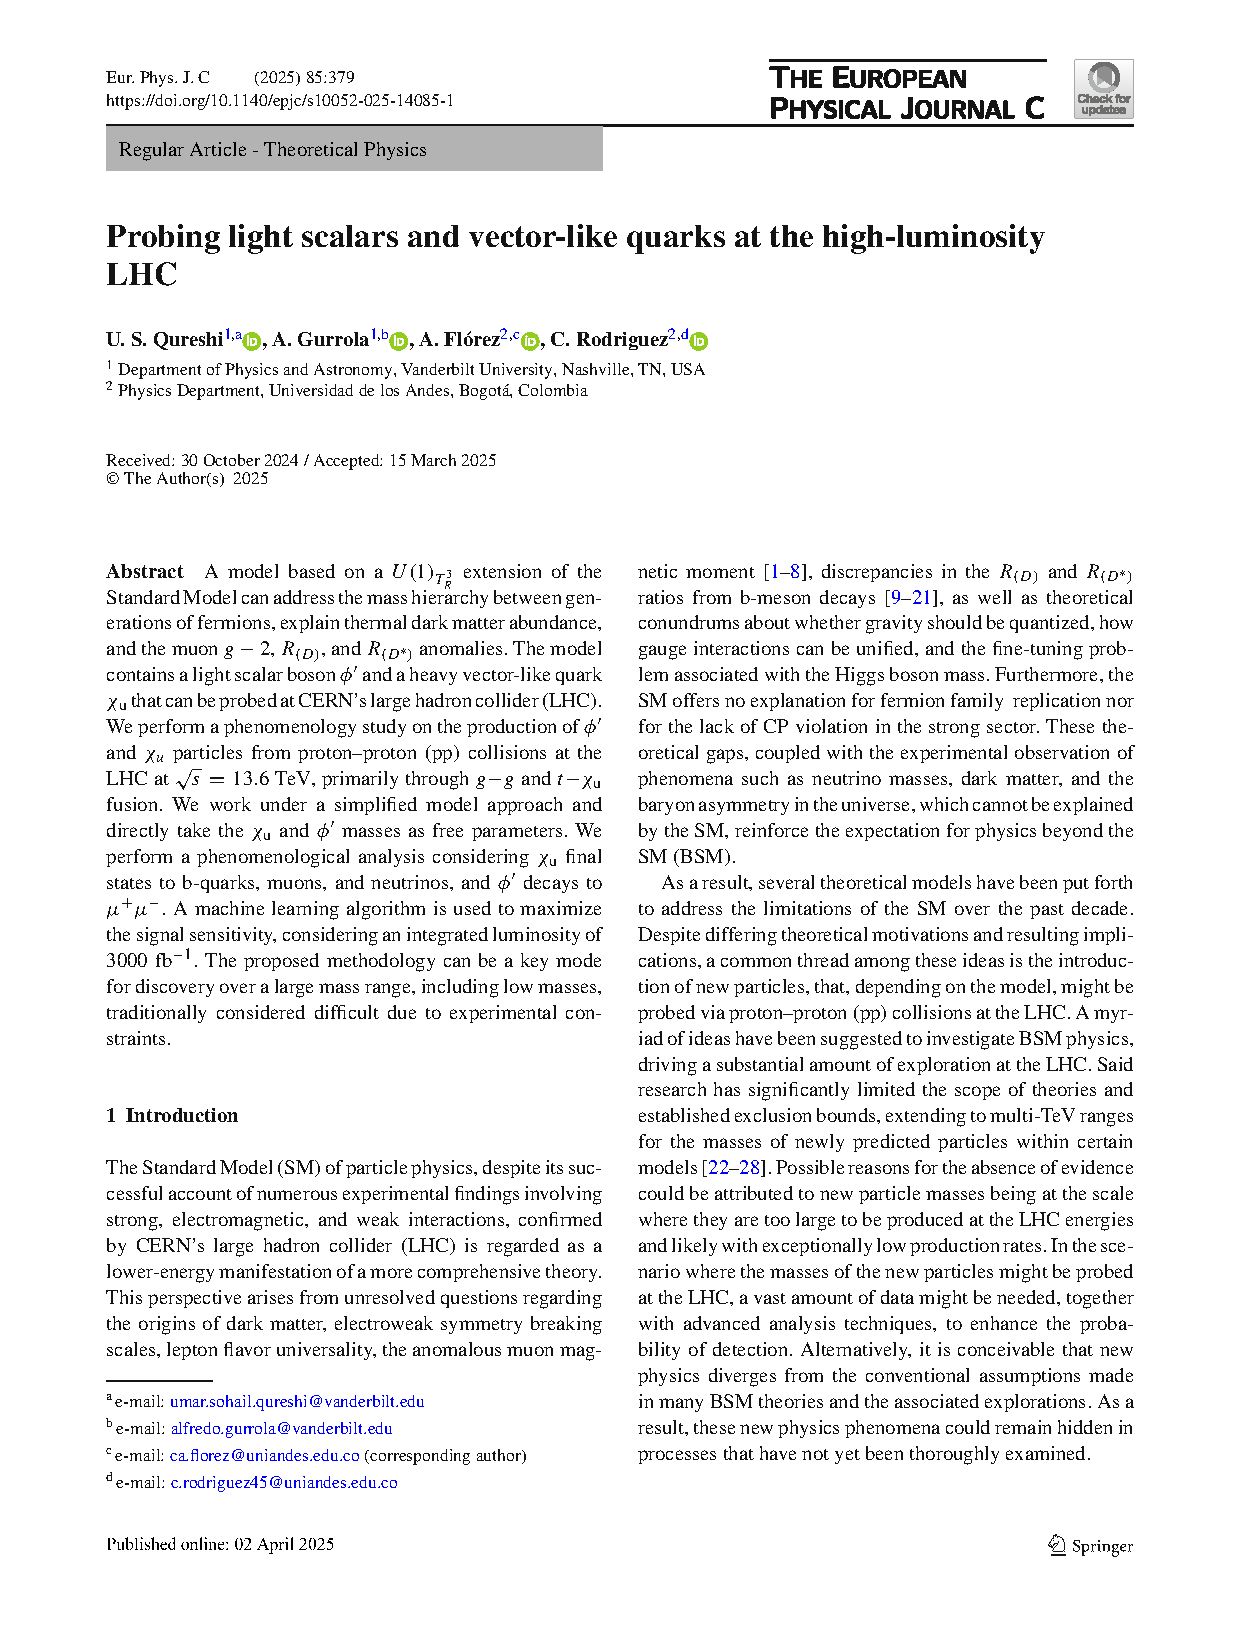
\includepdf[pages=-,link=true]{papers/s10052-025-14085-1.pdf} % Add more papers as needed
\end{document}
